% Load the kaobook class
\documentclass[
	fontsize=10pt, % Base font size
	twoside=false, % Use different layouts for even and odd pages (in particular, if twoside=true, the margin column will be always on the outside)
	%open=any, % If twoside=true, uncomment this to force new chapters to start on any page, not only on right (odd) pages
	secnumdepth=1, % How deep to number headings. Defaults to 1 (sections)
  toc=indentunnumbered % indent unnumbered entries in toc. if not used, they
                       % will be on the same indent as numbered parent entries
]{kaobook}

% Choose the language
\usepackage[english]{babel} % Load characters and hyphenation
\usepackage[english=british]{csquotes}	% English quotes

% === CUSTOM THINGS ===
\usepackage{mycommands}
\usepackage{nicefrac}
\usepackage{commath}  % for \abs and \norm, cf https://tex.stackexchange.com/a/149022
\usepackage{chemformula}
\usepackage{optidef}  % typesetting optimisation problems
\usepackage{hyperref}
\usepackage{listings}

\usepackage{amssymb} % for checkmarks

% Load the bibliography package
\usepackage[style=numeric,sorting=none]{kaobiblio}  
% \usepackage[style=numeric,sorting=none]{biblatex}
\addbibresource{./BA.bib}

\usepackage{subcaption}

% algorithm typesetting setup
\usepackage[linesnumbered,ruled]{algorithm2e}
\setlength{\algoheightrule}{0pt}
\setlength{\algotitleheightrule}{0pt}
% \SetCommentSty{\familydefault}
\newcommand\mycommfont[1]{\footnotesize \textcolor{teal}{#1}}
\SetCommentSty{mycommfont}

% ======

% Load packages for testing
\usepackage{blindtext}
%\usepackage{showframe} % Uncomment to show boxes around the text area, margin, header and footer
%\usepackage{showlabels} % Uncomment to output the content of \label commands to the document where they are used
  

% Load mathematical packages for theorems and related environments
\usepackage{kaotheorems}

% Load the package for hyperreferences
\usepackage{kaorefs}

\graphicspath{{images/}{./}{../GraphGym/run/}} % Paths where images are looked for

\makeindex[columns=3, title=Alphabetical Index, intoc] % Make LaTeX produce the files required to compile the index


\begin{document}

%----------------------------------------------------------------------------------------
%	BOOK INFORMATION
%----------------------------------------------------------------------------------------

% \titlehead{Document Template}
\title[Node Duplication in Disease Maps using Graph Neural Networks]{Node
  Duplication in Disease Maps \\ using Graph Neural Networks}
\author[BM]{Benjamin Moser}
\date{\today}
% \publishers{An Awesome Publisher}

%----------------------------------------------------------------------------------------

\frontmatter % Denotes the start of the pre-document content, uses roman numerals


%----------------------------------------------------------------------------------------
%	DEDICATION
%----------------------------------------------------------------------------------------

% \dedication{
% 	The harmony of the world is made manifest in Form and Number, and the heart and soul and all the poetry of Natural Philosophy are embodied in the concept of mathematical beauty.\\
% 	\flushright -- D'Arcy Wentworth Thompson
% }

%----------------------------------------------------------------------------------------
%	OUTPUT TITLE PAGE AND PREVIOUS
%----------------------------------------------------------------------------------------

% Note that \maketitle outputs the pages before here
\maketitle

%----------------------------------------------------------------------------------------
%	PREFACE
%----------------------------------------------------------------------------------------

\chapter*{Abstract}

%	One or two sentences providing a basic introduction to the field,
% comprehensible to a scientist in any discipline
% - systems biology, complex interplay, biological networks
% can do more specific with disease maps i think, we are more general in
% background
Many diseases are thought to arise through complex interactions of biological
processes or genetic and environmental factors.
% Two examples are Alzheimer's Disease and Parkinson's Disease.
% (not sure if this sentence is needed)
Knowledge on related processes and contributing factors
is often scattered throughout individual publications.
%
The set of biological entitites and the processes linking them naturally yields
a network.
Disease Maps are large-scale digital diagrams of such networks that
describe all processes relevant to a given disease in a formalised manner.
They serve as a
knowledge base for visual exploration and computational analysis.
% augmented with additional information such as
% links to individual publications or biological database entries.
% Two to three sentences of more detailed background, comprehensible to
% scientists in related disciplines
% - particularly diseases
% - knowledge repository
% - systematic overview of all known, involved processes
% One sentence clearly stating the general problem being addressed by this
% particular study.
% - node duplication to reduce hairball effects
% - important for
% -- semantic clarity
% -- layout (bunch of methods rely on that decision)
%
% curation and layout still commonly done by expert, very labor-intensive
% Although automatic methods are being developed, a
To date, finding a high-quality layout requires considerable manual
curation by experts.
% a considerable amount of manual
% curation by experts is still required to find a layout of high quality.
A possible means for improving a preliminary layout is to duplicate an
existing node and re-destribute its incident edges among the duplicates.
% The decision whether to duplicate a node hinges on its biological meaning
% layout factors
% semantic factors
The decision of whether to duplicate a node is commonly still left to the
expertise of a human curator. Previous work
% \cite{nielsen_MachineLearningSupport_2019}
suggests to employ a Machine Learning
% TODO cap. of ML
model trained on a set of already laid-out diagrams to predict node duplication.

In this work, we explore the usefulness of Graph Neural Networks (GNNs) for
predicting node duplication.
%
We assess which
of the features suggested in previous work
% \cite{nielsen_MachineLearningSupport_2019}
serve well as predictors,
%
and explore approaches to integrate biologically meaningful information in the
form of Gene Ontology term annotations.
%
Furthermore, we consider some variants of the basic GNN model and
additional techniques such as addressing class imbalance.
%
Finally, once a prediction has been made, we propose an approach to determine
the number of duplicates to be introduced and how to distribute incident edges
among the duplicates.

Our results show that GNNs provide little immediate advantage compared to the
Support Vector Machine approach of previous work. 
%
Further, we show that, in some tasks, using a sequence of reorganisation
snapshots taken during manual curation as training data is not beneficial
compared to simply using the single finished, fully laid-out diagram.
% Further, we show that when evaluating the classifier on a disease map in which
% every species has only a single visual representation, using a series of
% snapshots taken during incremental reorganisation of a disease map by an expert
% as training data is in fact not beneficial compared to simply using the final,
% fully curated map as training input.
%
We see that it makes little difference whether structural features such as node
centralities are calculated based on the bipartite graph interpretation of the
disease map or on its bipartite projection.
%
Next, we show that directed node degree is already a strong indicator for
node duplication in the considered data. However, using additional structural
features still marginally increases classification performance.
%
Exploiting Gene Ontology annotations remains challenging due to the complexity
and ambiguity of the provided information.
%
Our approach to determine the number of duplicates and attachment of incident
edges appears promising.



% One sentence summarizing the main result (with the words “here we show” or
% their equivalent)
% - applicability of more complex classifier (GNN) and techniques
% - assess importance of reorganisation steps for training
% - assess importance of features
% - try some new features
% - finally, attachment of edges

% Two or three sentences explaining what the main result reveals in direct
% comparison to what was thought to be the case previously, or how the main
% result adds to previous knowledge
% - (GNN about same performance of SVM)  not sure if should mention this because
% this is probably rather constrained by the data, not model capacities
% - dont need reorganisation steps when evaluating on collapsed maps
% - class imbalance does not seem to be a problem (at least could not be
% alleviated by providing weights)
% - degree alone alredy reaches close performance, but centrality and node class
% measures do give some little improvement
% - (how do we mention ontology features here?)

% One or two sentences to put the results into a more general context
% - remains an ill-conditioned problem
% - although results hint at that heuristics such as degree threshold are not
% too bad
% - ML tricky due to little draining data and low quality of data
% - but still effective, useful particularly for making suggestions

% Two or three sentences to provide a broader perspective, readily
% comprehensible to a scientist in any discipline, may be included in the first
% paragraph if the editor considers that the accessibility of the paper is
% significantly enhanced by their inclusion.
% - easier curation of disease maps super important
% - also for layout algorithms



% TODO somewhere (related work? background?) describe in more detail the
% use-case of nielsen of suggesting predictions (maybe even with screenshot)




%----------------------------------------------------------------------------------------
%	TABLE OF CONTENTS & LIST OF FIGURES/TABLES
%----------------------------------------------------------------------------------------

\begingroup % Local scope for the following commands

% Define the style for the TOC, LOF, and LOT
%\setstretch{1} % Uncomment to modify line spacing in the ToC
%\hypersetup{linkcolor=blue} % Uncomment to set the colour of links in the ToC
\setlength{\textheight}{230\vscale} % Manually adjust the height of the ToC pages

% Turn on compatibility mode for the etoc package
\etocstandarddisplaystyle % "toc display" as if etoc was not loaded
\etocstandardlines % "toc lines as if etoc was not loaded

\tableofcontents % Output the table of contents

% TODO include?
% if so, set up short captions.
\listoffigures % Output the list of figures

% Comment both of the following lines to have the LOF and the LOT on different pages
\let\cleardoublepage\bigskip
\let\clearpage\bigskip

% TODO include? probably not.
\listoftables % Output the list of tables

\endgroup

%----------------------------------------------------------------------------------------
%	MAIN BODY
%----------------------------------------------------------------------------------------

\mainmatter % Denotes the start of the main document content, resets page numbering and uses arabic numbers


\setchapterstyle{plain} % Choose the default chapter heading style

\pagelayout{wide} % No margins




\chapter{Introduction}
% see [[Writing Outline]]

% have to deal with duplicates due to some species appearing often
% and potentially involved in crosstalk

% duplicates are problem because (rephrase from what i wrote in background)

% tools already do support displaying or introducing duplicates

% but decision of duplication still up to the curator

% curating layout is insanely labour-intensive process

% distinction of use-cases (identify *all*, or few high-confidence suggestions)?
% how important is this even?


% bit of background, where are we, what is the problem
% \paragraph{Overview}
Deciding node duplication is an essential problem for
layouting large biological process diagrams such as disease maps. 
Commonly, this decision is still left to manual curation by an expert. Previous
work
\cite{nielsen_MachineLearningSupport_2019}
suggests to train a machine learning model to suggest to the human curactor
which nodes should be duplicated. In this work, we aim to extend this
approach in several directions. First, we explore the applicability of Graph
Neural Networks to this classification task. Second, we consider which of the
previously suggested features are useful and introduce a new set of features
based on Gene Ontology term annotations. Finally, we suggest an approach to
distribute edges after duplication.
% TODO this does not contain quite everything, go over sec 5 again


% \paragraph{Problem Statement} 
% what is the concrete problem we are tying to solve?
% state in a formal, precise manner
Our aim is to support the curation of disease map diagrams using a Machine
Learning model. Given a node in a diagram, the model predicts whether that node
should be duplicated.
%
We interpret a disease map as a directed, bipartite attributed graph in which
species aliases and reactions constitute the bipartite node sets. Nodes are
associated with annotations providing additional domain-specific information.
The graph representation also allows to compute structural characteristics such
as centrality scores.
%
For training the model, disease maps can be given in two variants: Either as a
single disease map, or as a sequence of reorganisation steps. Such a sequence is
made up of intermediate snapshots of a disease map taken during the curation
process. For evaluation, we always consider the variant of a single disease map.
% TODO motivate somewhere why --- not much data available
%
Additionally, nodes of the graphs in the training dataset are associated with
ground-truth labels indicating whether the node should be duplicated. Given one
or several such training graphs, we aim to train a classifier for \ild{binary
  node classification}, i.e. for making a prediction for nodes in previously
unseen graphs.
%
Moreover, assuming we are given the knowledge that a node should be duplicated,
we seek to find the number of duplicates to introduce, as well as how to
distribute the edges incident to the original node among its duplicates.
% (fragment)
% Moreover, finding the exact number of duplicates to introduce and how to connect
% them is not trivial and was commonly left to human curators. We provide a basic
% approach to answer this.

% (fragment)
% Further, it remains an open to question where to position the newly introduced
% duplicates in the layout. We leave this question to future work.

% \paragraph{Motivation for GNN Approach}

A layout can always be improved in terms of edge crossings, edge lengths or node
positions by duplicating nodes. However, duplicating a node and re-attaching its
incident edges potentially removes a path through that node. That path
may be semantically meaningful and in that case it should be represented
explicitly in the network structure.
The decision of whether a node should be duplicated hinges on
assessing whether such paths are meaningful or not, \ie whether the linkage via
a node establishes \ild{true} or \ild{false connectivity} of its neighbourhood.
Thus, the decision of node duplication ultimately depends on the context
(neighbourhood) of the node.
%
Due to the message-passing operations, a Graph Neural
Network is able to recognise patterns of node attributes across a local
neighbourhood. We hypothesize that the ability to learn such patterns may be
beneficial for capturing and generalising the decisions in the training dataset.

% Previous methods for deciding node duplication are typically based on setting a
% threshold on some measure
% that considers the context of a given node (see \nameref{sec:related-work}).


% \paragraph{Motivation for using Gene Ontology annotations}
We hypothesize that, in general, a node should be duplicated if its
neighbourhood is highly heterogeneous. In this case, false connectivity is
established between actually unrelated processes.
Previous approaches commonly focus on structural or layout-based features to
decide node duplication.
However, these facets involve domain knowledge only implicitly, if at all.
As a characterisation of neighbourhood heterogeneity, we seek
to explicitly include domain knowledge about what biological processes a species
is involved in. To this end, we consider the Gene Ontology (GO) terms linked to each
species in a given disease map. In particular, we consider the terms of the
\textit{biological process} subtree of the GO graph.
%
We represent a GO term by an embedding vector representing its position -- and
thus its semantics -- in the GO graph.
% We explore two approaches for using that
% information:
% \begin{itemize}
% \item We simply use the embeddings as node features. We hypothesize that a Graph
%   Neural Network may be able to capture characteristic neighbourhood patterns
%   that induce duplication.
% \item For a given node alias, we compute a measure of spread of the embeddings
%   of its neighbours. The idea is that the diversity of the neighbour's
%   embeddings may be an indicator for node duplication.
% \end{itemize}



% (fragment)
% As such, it is problematic to hinge the decision of duplication on the identitiy
% of the node alone, since the same species may be a connector in some cases and
% not in other cases. As elaborated above, we have to consider its neighbourhood.

% (fragment)
% Motivated by this, we seek to implicitly capture the criteria for node
% duplication by training a machine learning model on a sequence of snapshots of a
% diagram during a reorganisation process performed by an expert. The model is
% trained to predict whether a node should be duplicated or not.


% (fragment)
% While structural features such as an extremely large node degree
% immediately come to mind, such simple predictors often do not suffice to capture
% all cases (see \nameref{sec:experiments-results}).
% % TODO elaborate more?

% \paragraph{Structure}
We begin by reviewing the basic notions and definitions in
\refsec{background}. In \refsec{related-work}, we review related work from the
perspectives of Graph Drawing, Machine Learning and Ontologies.
We describe the actual methods employed for preprocessing, model training and
classification in \refsec{methods}. Additionally, we give a short overview over
our technical implementation of these methods. In \refsec{experiments-results},
we describe and discuss the performance of different approaches. Finally, we
conclude with a general discussion of results (\refsec{discussion}) and
possible directions for future work (\refsec{future-work}).







% TODO some prose on how biological systems are complex, inspired by
% https://www.quantamagazine.org/biologists-rethink-the-logic-behind-cells-molecular-signals-20210916/

% motivation for disease maps
% Our understanding of the molecular mechanisms that are involved in biological
% systems is improving drastically. However, this knowledge is growing
% incrementally and is often scattered across individual scientific publications.

% To properly consider complex signalling effects such as
% activation/inhibition, crosstalk or feedback, it is of the essence to make this
% network structure accessible to both human cognition and computational analysis
% \ cite{barabasi_NetworkBiologyUnderstanding_2004}.

% TODO node duplication important in
% - general network analysis, as preprocessing (manipur, iPAO1, ...)
% - visualisation

% may not be a good idea to simply duplicate anything e.g. involved in more than
% one pathway because of *key connectors*

% becomes particularly relevant now that we are layouting more than single
% pathways, general connectivity is importnat

% overview (this work is structured as follows blah)
% basic concepts given in background.
% mention that abbreviations etc are given in appendix
% position against other work in related work
% descibe approach in methods
% give experiments and results

\chapter{Background}
\label{sec:background}
In this section, we review the basic notions and definitions relevant for this
work. We introduce
biological networks in general, disease maps in particular and highlight
specific challenges that arise when working with such networks. Further, we
provide background on the classification models used in this paper. We motivate
and derive Graph Neural Networks based on the notion of neighbourhood
aggregation. We proceed by informally deriving the basic formulation of Support
Vector Machines and conclude with methods for evaluating the performance of
classifiers. Related work is reviewed in \refsec{related-work}.


\section{Biological Networks}
\label{biological-networks}
% NOTE already did one pass of editing

The behaviour of biological systems is often shaped by complex interactions.
% potentially across different levels of abstraction.
% In the most general sense, we refer to biological entities as \textit{species}.
%
% dont really need to list possible types if we give concrete examples below
% Possible species types are
% proteins, genes, but possibly also phenotype descriptions or drugs.
% %
% Possible relations include chemical reactions such as state transitions (e.g.
% phosphorylation), physical interactions between two proteins or the effect a drug
% has on the function of some protein.
%
%
The set of entities in a system and their interactions (relationships) naturally
form a network. We refer to a biological entity in such an interaction network
as a \ild{species}. Choices of what species and relationships to consider yield
different kinds of biological networks. To provide an overview, we describe some
prominent examples:
\begin{itemize}
\item \ild{Protein-protein interaction} (PPI) networks describe the complex
  interactions between different proteins. Analysing the entire network of
  interactions is interesting because the effective biological function of
  proteins is rarely defined based on their identity alone, but rather on their
  roles as enzymes or signalling molecules in relationship to other proteins.
  \textsc{PPI} networks can be useful to infer the biological function of an
  unknown protein or gene, or to group functionally similar proteins.
  % TODO more cites -- e.g. the thing from the context?
\item A \ild{metabolic model} of some organism consists of a formally described
  set of chemical compounds (\ild{metabolites}) as well as a set of chemical
  reactions or interactions between metabolites. Computational analysis
  methods on metabolic networks can be used to predict the growth of an organism
  under specific conditions, identify key intervention targets to alter
  metabolic processes, or identify relatively independent metabolic subsystems.
  % TODO citations
\item \ild{Disease maps} visually describe species and interactions that are of
  relevance to a specific disease. They serve as a comprehensive and coherent
  collection of existing knowledge that is otherwise scattered across individual
  publications.
\end{itemize}
Species and relationships need not necessarily have a direct physical
counterpart. Several works investigate the interactions between diseases, drugs,
or phenotypes, potentially connecting concrete physical entities (such as
proteins) to abstract entities (such as, for instance, drug side effects)
\cite{ruiz_identification_2021, barabasi_NetworkMedicineNetworkbased_2011}.
% TODO cite that work on gene classification for cancer thing presented by janina
% TODO cite more
Moreover, biological networks
% such as PPI networks or metabolic models
may serve as a scaffold to put data on individual species into relation with one
another.
% TODO example: manipur cancer classification, scRNA analysis
% maybe describe in one more sentence.
% to integrate data on, e.g., gene expression or reaction rates.
% This can be used to classify cancer
% TODO more precise and cite, the work I looked at for prop for whole-graph
% classification

\section{Disease Maps}

% what we want to say is: we already have (small) pathway diagrams, but they are
% not enough for describing a disease

Metabolic models or protein-protein interaction networks are abstract models.
They are given by formally described sets of species and interactions and are
thus well suited for computational analysis. However, the ability of human
experts to obtain insight from network data cannot be fully replaced. To this
end, it is necessary to find a representation of the abstract network that is
useful to the consumer. Most commonly, this means finding a visual
representation, that is, a \ild{drawing} of the network. Moreover, metabolic
models or PPIs are general models. Not all contained information may be relevant
for a given task, such as investigating the mechanisms behind some particular
disease. Particularly when presenting a wealth of data to human viewers, it is
important to focus on on the subsets that are relevant for the task at hand.

Individual biochemical pathways can be described visually by \ild{process
  description diagrams}. These typically involve less than a few hundred nodes
and edges. Species are represented as discs or boxes and are linked by lines
representing their relationships. Additionally, reactions may also be
represented by distinct graphical elements other than lines. We refer to the
visual representation of a species as a \ild{species alias}. Such diagrams have
traditionally been used to describe reaction cascades and metabolic subsystems,
first in the form of hand-drawn illustrations and later as computer-generated
graphics. An example is given in \reffig{process-diagram-old-vs-new}.

However, several diseases such Alheimer's Disease or Parkinson's Disease do not depend
merely on a single pathway. Rather, they are thought to arise through complex
interactions of biological processes or genetic and environmental factors.
Knowledge on relevant factors is obtained incrementally and scattered across
% TODO different word for relevant factors
individual publications or database entries.
Thus, a systematic understanding of the involved actors and their
relationships is essential
% it is of the essence to make this
% network structure accessible to both human cognition and computational analysis
% \ cite{barabasi_NetworkBiologyUnderstanding_2004}.
\cite{ostaszewski_CommunitydrivenRoadmapIntegrated_2019,
  mazein_SystemsMedicineDisease_2018}.
% 
For several diseases, experts have assembled \ild{disease maps}, comprehensive
visual diagrams combining all known mechanisms relevant for a given disease.
These diagrams are particularly suited for visual, interactive exploration. An
example is given in \reffig{process-diagram-old-vs-new}. A disease map can be
seen as a kind of biological process diagram. Note that a disease map may well
focus on describing metabolic processes or interactions between proteins. The
distuingishing property between disease maps and other, abstract biological
networks is that disease maps additionally provide an informative visualisation
of the network structure.
% TODO sort of implies that PPIs are biological processes
To summarise, disease maps differ in nature from other types of biological
networks in the following aspects:
\begin{itemize}
\item Disease maps are assembled based on the judgement of their curators. Only
  processes that are deemed relevant or informative to the given objective are
  included.
\item While other biological networks such as PPI networks or metabolic networks
  are defined mainly by their abstract network structure, a disease map is an
  actual visual diagram. Species and relationships have been laid out to
  optimally present the included information.
\item
  Recent disease maps contain up to several thousands of species and reactions and
  are very rich in information beyond the mere enumeration of species and their
  pairwise relationships. For example, a disease map may contain different types
  of species such as proteins, genes, phenotypes \etc. Species may have
  different states (e.g. ``phosphorylated'') and be nested in \ild{complexes}
  (groups). Further, species and relationships are often
  annotated with links to external databases such as Entrez Gene
  \cite{maglott_EntrezGeneGenecentered_2005} or UniProt
  \cite{theuniprotconsortium_UniProtUniversalProtein_2021}.
  This poses special challenges particularly for layout and
  interactive exploration. 
\end{itemize}

Traditionally, biological process diagrams have been drawn as pixel- or
vector-based graphics. Formalised, digital representations provide several
advantages:
\begin{itemize}
\item Creating a disease map requires a high amount of effort and domain
  knowledge. The extraction of knowledge from scientific publications or
  databases, as well as finding an adequate visual layout can be supported by
  computational tools.
\item Entities in the diagram may be annotated with additional information
  such as links to research publication or database entries.
\item A formalised representation enables the use of computational methods for
  analysis and interactive exploration (see \refsec{related-work}).
\end{itemize}

% TODO vertical alignment of subfigure labels
\begin{figure}[h]
  \centering
  \begin{subfigure}{0.4\textwidth}
    \centering
    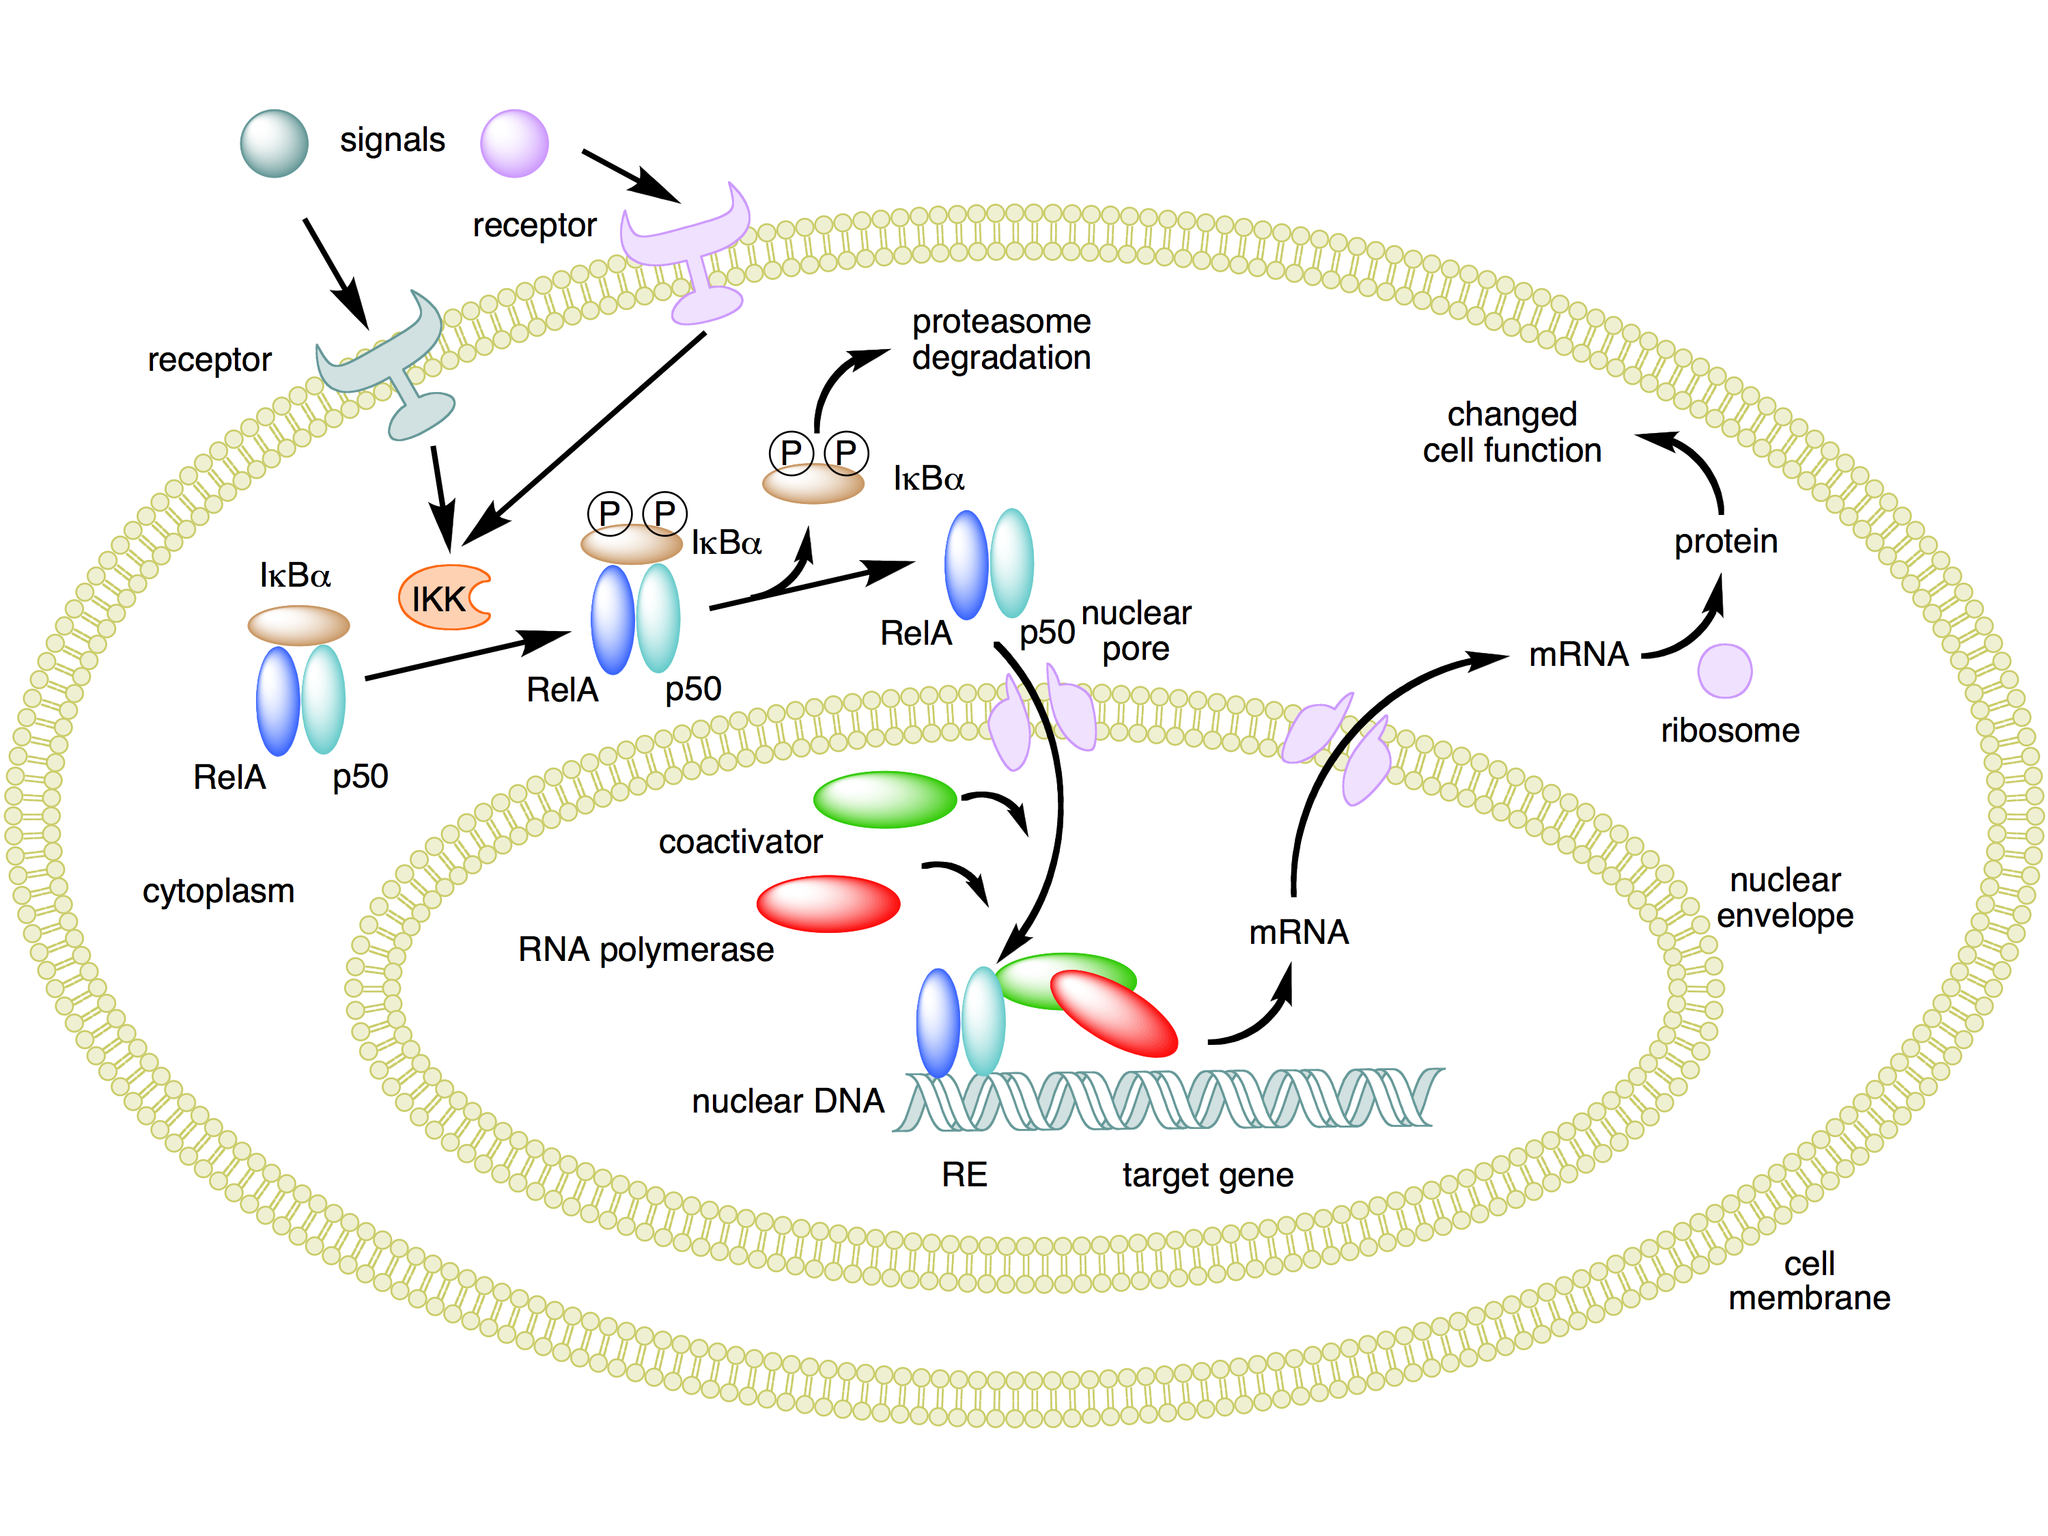
\includegraphics[width=\textwidth]{NF-kB-mechanism/handdrawn.png}
    \caption{Manually created diagram.}
    \label{fig:process-diagram-old-vs-new:handdrawn}
  \end{subfigure}
  \hspace{1em}
  \begin{subfigure}{0.4\textwidth}
    \centering
    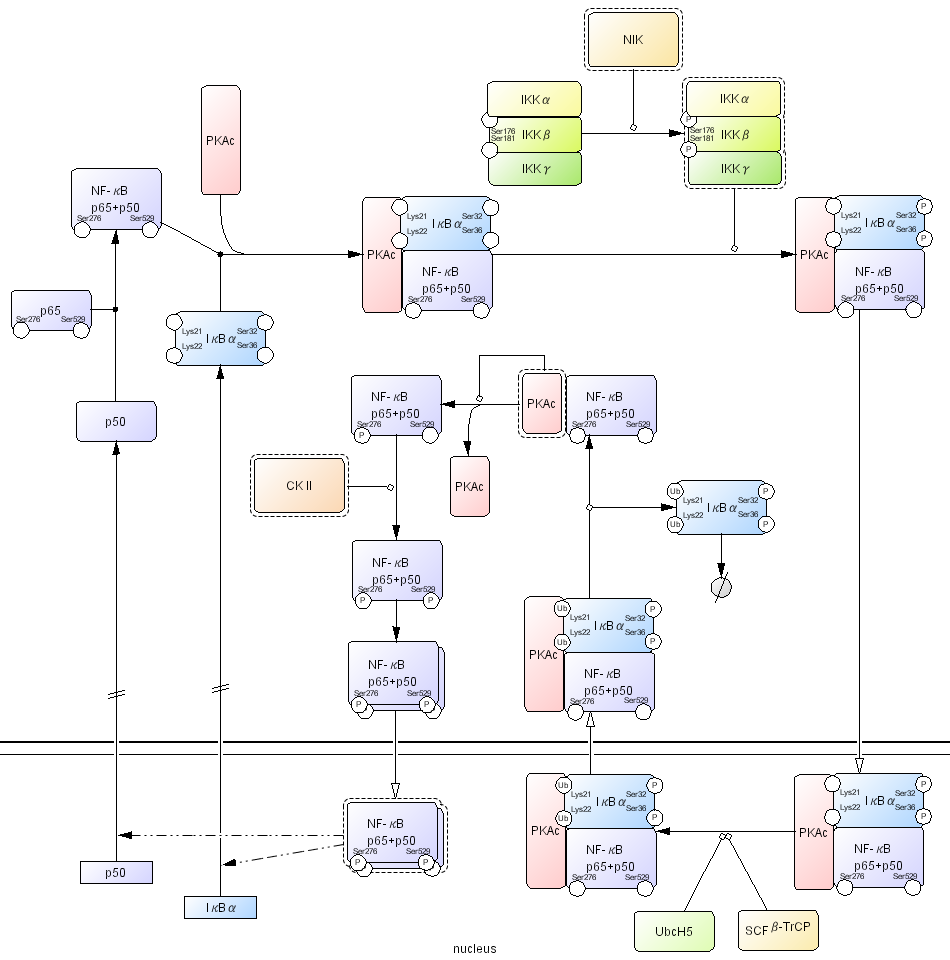
\includegraphics[width=\textwidth]{NF-kB-mechanism/CellDesigner.png}
    \caption{Diagram as created with \toolname{CellDesigner}. Species are
      represented as large, coloured boxes. Biochemical reactions are
      represented as arrows. }
    \label{fig:process-diagram-old-vs-new:celldesigner}
  \end{subfigure}
  \caption{
    Two representations of prototypical mechanisms of \nfkb{}-signaling.
    % TODO replace with sth that uses boxes for reactions
    % TODO describe roughly what this is for.
    % TODO descibe pros/cons of each
    % TODO describe why this is a nice example for a'' `complex interaction'
  }
  \label{fig:process-diagram-old-vs-new}
\end{figure}
% TODO replace with image from  http://www.celldesigner.org/features.html ?

\begin{figure}[h]
  \centering
  \pic{disease-map-screenshots/reconmap.jpg}
  \caption[Screenshot of the \textit{ReconMap}]{Zoomed-out view of the entire \textit{ReconMap}, a
    diagram describing the human metabolism
    \cite{noronha_ReconMapInteractiveVisualization_2017}.}
  \label{fig:disease-map-example}
\end{figure}
% \begin{figure}[h]
%   \centering
%   \pic{disease-map-screenshots/pdmap-excerpt.png}
%   \caption[Excerpt of \PDMap (Parkinson's Disease)]{Excerpt of \PDMap
%     \cite{fujita_IntegratingPathwaysParkinson_2014}, describing molecular
%     mechanisms of Parkinson's Disease.}
%   \label{fig:pdmap-example}
% \end{figure}

Because of the complexity of the contained information, finding a drawing for a
disease map that is suited for visual exploration is not trivial.


% -------------------------------------
\section{Drawing of Biological Process Diagrams}
\label{sec:draw-biol-netw}

Network-structured data can be represented formally as a \ild{graph} given by a
set of entities (\ild{nodes}) and a set of relationships(\ild{edges}).
%
The most widely used and intuitive visualisation paradigm is the
\textit{node-link diagram} in which nodes are represented graphically as dots,
circles or boxes and edges are represented by lines. For sake of simplicity, we
use \textit{nodes} and \textit{edges} ambiguously both in their mathematical
sense and for their graphical representations.
%
Finding a \textit{layout} of a graph (also called \textit{graph drawing}) means
finding positions for node representations and potentially also routing edges.
%
What makes a good layout generally depends on the specific kind of network data and the
task of the consumer of the visualisation.
%
In general, a good layout is commonly required to avoid edge crossings or
overlapping nodes, to be compact and to keep euclidean distances proportional to
graph distances.
% TODO citation here?
Additional constraints may be for example the preservation of symmetries, clear
representation of hierarchical structure or preservation of a viewer's mental map when
updating a dynamically changing graph layout.
%
Automatic graph layouting is a highly studied topic and numerous different
methods are available (see \refsec{related-work}).

Biological process diagrams, however, often contain subgraphs with particular
semantics, which must be considered explicitly in the layout in order to convey
the contained information as effectively as possible.
Because of this, it is still common practise to draw such diagrams manually,
or to obtain an initial automatic layout and adjust that manually. This process is
extremely time-consuming and often requires specific domain knowledge.
We outline some of the challanges in drawing biological process diagrams
\cite{bourqui_MetabolicNetworkVisualization_2007,
  siebenhaller_HumanlikeLayoutAlgorithms_2020,
  wu_MetabopolisScalableNetwork_2019}:

% TODO clarify: talking about process diagrams here but applies as well do
% disease maps

\begin{itemize}
% \item Process diagrams may be created to convey or highlight particular
%   information and express an intentional message.
 \item Large diagrams such as the disease maps considered in this work often
   exhibit a clear structural and visual hierarchy.
 \item Biochemical reactions often involve main substrates and products as well
   as secondary cofactors and enzymes. Substrates and products are usually
   placed orthogonally on opposite sides while cofactors and enzymes are
   placed on the side.
 \item Biological pathways often involve reaction cascades. These should be
   displayed such that the cascade is distuingishable and easy to follow.
   It may be preferrable to align cascades to the natural reading direction of
   the viewer (commonly \textit{top-to-bottom} and \textit{left-to-right}).
 \item Some biological pathways involve cyclic patterns and these should be
   clearly distuingishable as such.
\item Biological process description diagrams may contain more information
  than merely species and reactions. Species can be (recursively) grouped
  into complexes. A complex is commonly represented as a box containing the
  visual representation of the species and thus its contents also need to be
  laid out. Further, cellular compartments are also commonly represented
  visually as large boxes or frames containing the biological processes
  therein. Since transport in and out of the compartment and other reactions
  involving the membranes are of high biological relevance, proper placement
  of nodes and edges inside, outside or on the boundary of compartments is critical.
  % already bit relevant to node duplication
\item It may be the case that a single species often is involved in several
  different biological processes. It may be preferrable to represent that
  species by multiple, separate visual representations.
\end{itemize}

The question of if and when to represent a species by multiple different visual
representations instead of a single one is exactly the focus of this work.


\section{Node Duplication \& Connectivity}

If the same species $S$ is involved in several different biological processes,
$S$ may either be represented by a single visual representation and linked to
all involved processes, or it may be represented by multiple visual
representations, each linked only to some processes.
%
In any case, each path through $S$ defines a connectivity
between the involved processes.

However, it may be the case that some processes involve the same
species, but that species' role is completely unrelated between the two
processes. This is the case, for instance, if the processes involve different
physical instances of that species, if the species is available in such
abundance that the actual physical instance is irrelevant, or if the species is
merely an unimportant byproduct.
% different physical identities
% potentially same, but irrelevant

Thus, if a species $S$ is involved in multiple processes, we need to assess
between which of these processes there exists in fact a \ild{true connectivity}
via $S$; or which merely involve $S$ in different, unrelated contexts
(\ild{false connectivity}).
%
True connectivity should be represented in the network structure and the visual
diagram as a path through $S$. There should be no edges implying false
connectivity.
False connectivity can be resolved by introducing another visual representation
for $S$ and re-attaching any incident edges. We refer to this procedure as
\ild{node duplication}.

These considerations are important for finding a faithful diagram layout.
If the number of involved processes is large, having only a single graphical
representation for $S$ may lead to a high amount of visual noise in the diagram: there
may be a large number of edges, covering a long distance and linking actually
completely unrelated processes.
%
Having many independent representations
certainly makes it easier to avoid visual noise. However, connections between
different subgraphs may no longer be encoded explicitly, omitting crucial
information from the diagram.

The criteria for deciding between true and false connectivity, and thus node
duplication are not immediately clear. In practise, the decision is made by
experts case-by-case, or general heuristics are employed (see
\refsec{related-work}). In this work, we aim for a more precise approach to
decide node duplication automatically in the context of disease maps.



% -------------------------------------
\section{Biological Databases and Ontologies}
\label{sec:ontologies}

% (mainly introduce gene ontology)

% main motivation: research projects deal in principle with the same entities
% (e.g. all mean the same type of ATP molecule), but entities are usually still
% described in natural language (as strings). Same holds for relationships.

% this is problematic becaus string representations are ambiguous and tricky to
% process / compare / identify
Different research projects on the same organism or disease deal in principle
with the same universal sets of biological entities and relationships. For
instance, if two projects were to describe the metabolic network of \ecoli, both
are likely to mention the function of Adenosine Triphosphate (ATP), a basic
molecule that appears in many metabolic reactions. Both projects use the same
notion of ATP and its effects, yet they may describe it differently, e.g., by
its full name, abbreviation or
% TODO commas for e.g.?
chemical formula. This hinders knowledge transfer and -integration. We are
striving towards a structured, formalised body of knowledge for representing
information about physical entities such as molecules, but also on biological terms
describing processes (e.g. ``glycolysis''), localisation (e.g. ``cytoplasm'') or
functions.
% TODO not nice, maybe example for functions

There are several publicly available databases that gather information on
biological entities such as proteins (\toolname{UniProt}
\cite{theuniprotconsortium_UniProtUniversalProtein_2021}), genes
(\toolname{EntrezGene} \cite{maglott_EntrezGeneGenecentered_2005}) or drugs
(\toolname{DrugBank} \cite{wishart_DrugBankKnowledgebaseDrugs_2008}). These
databases often gather basic information and related research about the entity.
% maybe https://sci-hub.st/10.1002/0471250953.bi0101s50

Likewise, biological terms describing processes, functions or cellular
localisation can be represented in an \ild{ontology}, a (directed acyclic) graph
of terms and their relationships. For instance, the terms ``glycolysis'' and
``carbohydrate metabolic process'' may be connected by a \textit{involved-in}
relationship. The Gene Ontology project \cite{ashburner_GeneOntologyTool_2000}
provides three distinct ontology graphs describing molecular functions, cellular
component or biological processes. Each ontology graph loosely describes a
relationship, however, links between hierarchies may also exist, for instance
that the DNA repair process occurs in the Mitochondrion.
% TODO do need to make clearer what'' `function' stands for.




\section{Supervised Learning for Classification}
\label{sec:supervised-learning}
Our goal is to predict whether a species alias in a disease map
should be duplicated or not. For each species alias, we extract 
\textit{features}, which we deem to be characteristic for the target label of
the node (see \refsec{feature-selection}).
Additionally, we are given training
data in the form of one or several disease maps and a binary label for each
species alias describing whether it was duplicated during manual curation. We
aim to use this training data to fit a machine learning model such that it will
be able to make meaningful predictions for species aliases in other disease
maps.

Thus, we are working in the setting of \ild{supervised learning}, which we
briefly introduce in the
following~\cite{vapnik_PrinciplesRiskMinimization_,bronstein_geometric_2021}:
% TODO better-looking references?
We consider $n$ observations $\mathcal{T} = \{(\vec x_i, y_i)\}_{i=1}^n$ (also
% TODO this would be saying we evaluate on data we trained with, lets phrase
% this better.
called \ild{training data} or \ild{examples}) to be drawn from an (unknown)
distribution $P$ over $\mathcal{X} \times \mathcal{Y}$ where $\mathcal{Y}$ is
the label domain and $\mathcal{X}$ is the feature domain. For the scope of this
work, we restrict ourselves to the \ild{binary classification problem}, i.e.
$\mathcal{Y} = \{0,1\}$ . We assume that $\mathcal{X} = \mathbb{R}^d$ and the
number of dimensions $d$ is large. Let us denote the set of
observed \ild{ground-truth} labels as $\mat Y := \{y_i\}_{i=1}^n$ and the set of
observed feature vectors as $\mat X := \{x_i\}_{i=1}^n$. $\mat X$ can also be
seen as a matrix in $\mathbb{R}^{n \times d}$.
%
We assume that labels are generated by an unknown function $f$ such that $y_i
= f(\vec x_i)$.
%
Further, we are given a \ild{loss function} $\mathcal{L} :
\mathcal{Y} \times \mathcal{Y} \rightarrow \mathbb{R}$ that describes how
different a prediction is from the true outcome.
%
In general, we aim to find a (parameterised) function $\tilde f$ that minimises
the \ild{true risk} $\mathcal{R}(\tilde f) := \mathbb{E}_P\left[ \mathcal{L}(y_i,
    \tilde f(\vec x_i)) \right]$, where $\mathbb{E}_P$ is the expected value
over $P$.
%
Since the original distribution $P$ is unknown, we instead seek to minimise the 
 \ild{empirical risk} on the training data
$\mathcal{R}_{\text{emp}}(\tilde f) := \nicefrac{1}{n}
\sum_{i=1}^n \mathcal{L}(y_i, \tilde f(\vec x_i))$ and assume the empirical risk
approximates the true risk.
%
In the following, we call a concrete choice of $\tilde f$ a \ild{model} or a
\ild{classifier}. $\tilde f$ is commonly parameterised by a set of \ild{model parameters}
$\theta$.

For finding the classifier $\tilde f$, we can choose out of a variety of
existing approaches. The two model families we consider for classification in
this work are graph neural networks and Support Vector Machines. We describe
these in detail in the following sections.
% TODO captialisation


% TODO add a sentence that we evaluate on another set.


% TODO does this still apply? how does this relate to MLE as introduced via the
% BCE loss?


% -------------------------------------
\section{Graph Neural Networks}
\label{sec:neural-networks}

% The terminology used is still developing. There are many ways in which neural
% networks may exploit graph structure \footnote{
%   For instance, we do not consider here the mechanism of \ild{pooling} through
%   which the input graph can be coarsened w.r.t to its latent features.
% \cite{ying_hierarchical_2019}
% This is another idea that has a correspondence in CNNs
% \cite{zhang_dive_nodate}
% }. In this text, we will refer to neural
% networks that make use of message-passing layers in the style of
% \refeq{gnn-framework} as \ild{Graph Neural Networks}. Although the naming is
% somewhat ambiguous, this is the commonly used keyword.

% introduce neural nets as classifier here

A possible family of models that can be employed for classification is that of
\textit{neural networks}. A particular flavour of neural networks that we
consider in this work are \ild{graph neural networks}. We introduce basic neural
networks by example of one of its simplest variants, the \ild{multilayer
  perceptron}, or \ild{fully-connected neural network}. We then
introduce the notion of convolutions on grid-structured data and proceed to
generalise the intuition to graph-structured data, yielding the class of graph
neural network models. We proceed to describe how GNN models can be used for
node classification. The derivations are based on \citeauthor{zhang_dive_nodate}
\cite{zhang_dive_nodate} and \citeauthor{bronstein_geometric_2021}
\cite{bronstein_geometric_2021}.


\paragraph{Neural Networks}
The most basic building block of any neural network is a single \ild{neuron},
which is defined as the composition of a linear transformation with a nonlinear
\ild{activation function} $\sigma$. Formally, for a single input vector $\vec
x_i$, the output of a single neuron is given by $\sigma(\vec x_i^T \vec w + \vec
b)$ where the vector $\vec w$ is said to contain the \ild{weights} of the linear
transformation and $\vec b$ is the \ild{bias}. The stacking of multiple neurons,
of which each takes $\vec x_i$ as input, constitutes a \ild{fully-connected} or
\ild{dense} \ild{layer} in a neural network. If inputs and weights are stacked
in matrices $\mat X$ and $\mat W$, respectively, the output of a single layer is
given by $\sigma(\mat X^T \mat W + \vec b)$ where $\sigma$ is applied
element-wise.
%
A neural network is obtained by stacking multiple layers sequentially, such that
the output of one layer is the input to the next layer. The output of an
intermediate layer is commonly called \ild{latent} or \ild{hidden}
\ild{representation}. Formally, if $\mat H^{(i)}$ is the output of the $i$-th layer,
then the output of the $(i+1)$-th layer is given as
\begin{align}
\mat H^{(i+1)} = \sigma((\mat H^{(i)})^T \mat W^{(i+1)} + \vec b^{(i+1)}).
\label{eq:fully-connected}
\end{align}
% TODO sounds too much like what I wrote in the report?
%

\paragraph{Training} The layer weights $\Theta = \{\mat W^{(1)}, ...,
\mat W^{(l)}\}$ are considered to be the model parameters $\theta$ in the sense
of the supervised learning framework described in \refsec{supervised-learning}.
We aim to find a set of parameters such that the empirical risk is minimised.
% TODO empirical risk vs BCE loss function
This objective can be
optimised by \ild{Gradient Descent}: We iteratively adjust the weights
% $\mat W^{(i)}$
such that the model prediction is improved with respect to the empirical risk
$\Remp$. In the context of neural networks, $\Remp$ is also sometimes called the
total \ild{loss}, not to be confused with the loss function $\mathcal{L}$. More
precisely, we consider the partial derivative of $\Remp$ with respect to each
weight matrix, and iteratively update the weights for a maximum number of steps
or until the risk no longer improves. We can additionally specify the step size
by a given \ild{learning rate} $\eta$. Formally, in each step, also called
\ild{epoch}, we set
\begin{align*}
\mat W^{(i)}' \gets
\mat W^{(i)} - \eta \frac{\partial \mathcal{R}_{\text{emp}}}{\partial \mat W^{(i)}}.
\end{align*}

\paragraph{Hyperparameters} Characteristics such as the number of layers, the
number of neurons in each layer, or the choice of loss function and learning rate
determine the \ild{model architecture} and are called
\ild{hyperparameters}. The proper choice of hyperparameters is essential to the
performance of the model and often determined empirically via search techniques.

\paragraph{Automatic Feature Extraction and Message-Passing}
In practise, selecting suitable features is in itself a substantial
step in the process of finding a well-performing classifier.
%
Particularly in high-dimensional domains, feature selection is not trivial.
Consider the use-case of trying to find a model that, given a grayscale pixel
image of dimensions $(w, h)$, classifies the image based on whether it depicts a
dog or a cat. It is not trivial how to manually extract features (criteria) from
the image that are predictive of the target class. One possible approach
would be to consider the brightness value of each input pixel as a feature, i.e.
$\vec x_i \in \mathbb{R}^{w \cdot h}$. However, looking at each
pixel in isolation is unlikely to be useful since certainly the target class
depends on the values of pixels in their context.
% TODO moreover, extremely expensive if using MLP
Further, note that the hidden representation of some input (e.g. given by
\refeq{fully-connected}) may be considered an alternate feature representation
of this input. In this sense, neural networks can be thought to perform
\ild{automated feature extraction}. 


\paragraph{Convolutions on Grids}
For sake of intuitive appeal, let us further entertain the example of
classifying pixel graphics. We assume each pixel contains only one channel of
information and denote an image of size $(w,h)$ as a $w \times h$ matrix $\mat
X$. Analogous formulations can be used for other kinds of structured data,
including 1-dimensional grids (sequences) such as RNA and DNA sequence
alignments~\cite{flagel_UnreasonableEffectivenessConvolutional_2019,aoki_ConvolutionalNeuralNetworks_2018}.
It is important to note that we have additional information on the structure of
the input,
% (also called \ild{inductive bias}),
% TODO that term is not relevant here? would just sound fancy
namely that its pixel values are arranged in a grid. This means there is a
well-defined notion of context, or \textit{neighbourhood}.
%
Aggregating information across a local neighbourhood may enable
a model to capture not only characteristics of individual pixels but
higher-order patterns. To faithfully extract local patterns, the aggregation
operation should be \ild{local} (the aggregation considers only a part of the
input image) and \ild{translation invariant} (the aggregation responds
similarly to the same input patch, regardless to where the patch is positioned in the
entire grid). In the context of neural networks, such an aggregation is called a
\ild{convolution} \cite{zhang_dive_nodate}. In the case of linear aggregation
and grid-structured data, we can express a convolution operation centered on pixel $\mat
X_{i,j}$ as
\begin{align}
  \mat H_{i,j} = u + \sum_{a= -\Delta}^\Delta \sum_{b = -\Delta}^\Delta \mat V_{a,b} \mat X_{i+a,j+b}
  \label{eq:convolution}
\end{align}
% TODO diagram / illustration for grid convolution
where $u$ is the bias, and $\Delta$ is the (window) \ild{size} of the
\ild{convolution kernel} $\mat V$.
%
Note that the kernel can be any
computation adhering to the constraints of locality and translation invariance.
%
\refeq{convolution} describes a
\ild{convolutional layer} and a neural network containing such layers is called
a \ild{convolutional neural network} (CNN).

In image classification, a single input to the neural network is typically an
entire image (a collection of pixels), and the convolution operator is applied
to each pixel. 
%
Successive application of convolutional layers,
potentially with different kernels can be thought to aggregate increasingly
higher-order patterns in the input data. Additionally, the information of a
local neighbourhood can be aggregated into a lower-dimensional value by
\ild{pooling} operations.
%
The extracted patterns can be
considered intermediate, higher-order feature representations and successive
convolution operations extract increasingly higher-order features.
%
Since a kernel computes a value for a given pixel based on the features of
itself and its neighbours, we can interpret the operation of a kernel to perform
\ild{message-passing}: Neighbour nodes construct and transmit messages to the
target node, which are then combined with the target node's features into the
final output.


% TODO note somewhere that 'spectral' GNNs have been around for a while, but
% GNNs have only become quite popular recently with these simplified formulations
\paragraph{Convolutions on Graphs} We extend the notion of a convolution
from grid-structured graphs to arbitrary simple graphs. We will see that
the convolutions considered here are trivially local and translation invariant.
The key differences are that the order and the size of the neighbourhood is no
longer fixed. As such, a potential aggregation must be \ild{node-order
  invariant}.

Let us consider an attributed graph
$G$ with node set $V$.
% $G=(\mat X, V,E)$ with node set $V$, edge
% set $E$ and $d-dimensional$ attributes $\mat X \in \mathbb{R}^{\norm{V} \times
%   d}$.
Let $\vec h_i$ be the (intermediate) feature representation of vertex $v_i \in
V$. Let $\mathcal{N}(v)$ be some neighbourhood of $v \in V$. Typically,
$\neighb(v)$ is chosen as the 1-hop adjacency in $G$. However, note that
different notions of neighbourhood can also be applied, so the input graph must
not necessarily correspond directly to the computation graph that defines how
messages are passed. or instance, \textsc{GraphSAGE}
\cite{hamilton_InductiveRepresentationLearning_2018} samples a fixed number of
adjacent nodes. We can describe a simple convolution operation on $G$ as
follows: the new latent representation $\vec h_i'$ of $v_i$ is based on messages
received by its neighbours. Each neighbour encodes its attributes by means of a
function \textsc{Msg}. These messages are aggregated using a
permutation-invariant aggregation function \textsc{Agg}.
Finally, the neighbours' input and the node's own features $\vec h_i$ are
coalesced via an update function \textsc{Update} into the new latent
representation $\vec h_i'$. If we consider each node to be part of its own
neighbourhood, this can be summarised as:
\begin{align}
  & \vec h_i' \gets \textsc{Update}(\textsc{Agg}(\{\textsc{Msg}(\vec h_j, \vec h_i) ~|~ j \in \mathcal{N}_i\}))
    \label{eq:gnn-framework}
\end{align}
Concrete choices of \textsc{Msg}, \textsc{Agg} and \textsc{Update} give
implementations of \ild{graph convolution layers}. A neural network containing
such layers is commonly called a \ild{graph neural network} (GNN)
or \ild{graph convolutional network} (GCN).

In simple GNN architectures, \textsc{Msg} is a linear feature extraction and depends
only on the sending node, i.e. $\textsc{Msg}(\vec h_j, \vec h_i) = 
\mat W \vec h_j =: \msg_j$ for some learnable weight matrix $\mat W$. Note that
like the kernel parameters $\mat V$ in \refeq{convolution}, these weights are
shared among the message-passing operations of different nodes.
% 
\textsc{Update} is the application of a non-linear activation function and
\textsc{Agg} is given by
\begin{align*}
  & \textsc{Agg}(...) = \bigoplus_{j \in \mathcal{N}_i} \alpha_{ij} \vec{msg}_j,
\end{align*} where $\alpha_{ij}$ is a coefficient determing the importance of
$\vec{msg}_{j}$.


The framework of \refeq{gnn-framework} produces a hidden feature representation
for each node. This is the basis for solving node-level tasks such as the
classification of clustering of individual nodes. Another common use case is to
make a prediction for the entire input graph, the most prominent example in
context of life sciences being molecule graphs. In this case, we want to
aggregate all node features to produce a single value describing the input
graph. Like in CNNs, such an aggregation is called a \ild{pooling} layer. This
can be done either by application of a simple permuation-invariant aggregation
function or by iteratively coarsening the graph together with its node-level
feature representations \cite{ying_hierarchical_2019}.

% TODO also mention edge-level tasks and computation over edges,
% see https://distill.pub/2021/understanding-gnns/#modern-gnns > modern GNNs >
% thoughts for some references

\paragraph{Simple GNN} The \ild{GCN layer}, as
proposed by \citeauthor{kipf_semi-supervised_2017}
\cite{kipf_semi-supervised_2017}, defines $\alpha_{ij}$ as a constant depending
on the degrees of $v_i$ and $v_j$, namely $\alpha_{ij} := \nicefrac{1}{\sqrt{d_i
    d_j}}$.

\paragraph{GNNs with Attention} The \ild{Graph Attentional Layer} (GAT)
\cite{velickovic_graph_2018} allows the importance score $\alpha_{ij}$ to be learnable, i.e.
adjusted via backpropagation and gradient descent during network training. An
attention mechanism $A$ determines the importance $e_{ij}$ of $\vec{msg}_{ij}$.
If the neighbourhood $\mathcal{N}_i$ is defined as the 1-hop-neighbourhood in
the input graph, this can also be interpreted as the importance of edge $(v_i,
v_j)$. In its prototypical formulation, $A$ is a single-layer fully-connected
neural network with learnable weights $\vec a$ and activation function
$\sigma_{\text{att}}$. $A$ receives
both the feature representations of $v_i$ and $v_j$ as input, combined by
concatenation:
\begin{align}
  e_{ij} := A(\msg_i, \msg_j) = \sigma_{\text{att}}(\vec a^T( \msg_i \concat \msg_j))
\end{align}
Importance scores $e_{ij}$ are obtained by normalisation with the \ild{softmax} function:
\begin{align}
  \alpha_{ij} := \softmax_{j \in \mathcal{N}_i}(e_{ij}) := \frac{\exp(e_{ij})}{\sum_{k \in \mathcal{N}_i} \exp(e_{ik})}.
  \label{eq:softmax}
\end{align}
% NOPE: mention multi-head attention?
Attention is a technique that has previously been used successfully in other
neural network architectures. In particular, Graph Attention Networks are
analogous to the Transformer architecture \cite{vaswani_AttentionAllYou_2017}
that has achieved great popularity in areas of Natural Language
Processing such as machine translation.
% TODO capitalisation
For translation from a source language
to a target language, text input is typically given as two sequences of tokens.
The key idea behind the Transformer architecture in NLP is to apply an attention
mechanism to assess the importance of other words in the source or target
sequence with respect to the current word.
% NOPE diagram like in https://docs.dgl.ai/tutorials/models/4_old_wines/7_transformer.html
%   to illustrate message-passing of transfomer?
Note that while the Transformer architecture relies heavily on the attention
mechanism, it also directly implements the idea of message-passing based on
known relationships between atomic inputs.

Graph Neural Networks allow us to apply common Deep Learning techniques to
graph-structured data. For node-level learning tasks, this allows us to consider
the explicit relationships between individual nodes. For graph-level tasks such
as graph classification, GNNs are able to process the entire graph without
relying on a fixed-length encoding. Furthermore, the aggregations are invariant
to permutation and rotation.

% TODO GNNs relatively low complexity, seem to not need super-deep convolutions like w/images

% NOPE dont go into polynomial filters for graphs here but mention them in
% related work, the distill article gives a nice journey there that we can
% transcribe: https://staging.distill.pub/2021/understanding-gnns/

% NOPE
% \begin{figure}[h]
%   \centering
%   (diag-surfaces) on paper
%   % -- features in isolation
%   % — convolution on grid (like in dive 6.2.1)
%   % — 'convolution on sequence' (like in Transformer)
%   % can we find biological sequence here?
%   % — convolution on graph
%   % — neighbourhood on some other shape (maybe 3D shape)
%   % see (diag-surfaces) on paper
%   \caption{Including known structure into the ML model as predictive bias.}
%   \label{fig:diag-surfaces}
% \end{figure}


% having this geometry is an additional information/bias we give to the network/model

% can consider more complex geometries/surfaces → gauge-equivariant models
% allow to properly model rotations etc (``respect underlying symmetries''')

% are saliency maps an example for node-level task in image processing?
% starting point: https://medium.com/stellargraph/https-medium-com-stellargraph-saliency-maps-for-graph-machine-learning-5cca536974da

% TODO or on intermediate scale, finding
% communities, subgraphs, motifs, ... 

\paragraph{Neural Networks as Classifiers} We now consider how graph neural
networks can be employed for node classification. In each training epoch, the
neural network receives as input the node feature vectors and the graph's
adjacency matrix.
%
Intermediate layers of neural
networks can be interpreted to compute useful feature representations. One way
to obtain a classification prediction from a neural network is to use these
intermediate representations as an input to another off-the-shelf classifier
(such as Support Vector Machines, for instance
\cite{liu_CombiningConvolutionalNeural_2018}). Another, more common approach,
however, is to design the network such that the last layer contains one ouput
neuron for each target class. Given some input $\vec x$, the output value of the
$i$-th neuron expresses the estimated probability that $\vec x$ is of class
$c_i$. To produce values in $[0,1]$, the results of the final layer are
normalised, e.g. with the \textit{softmax} function (see \refeq{softmax}).
%
In order to train the neural network for classification, we need a loss function
$\mathcal{L}$ to assess the quality of the prediction. We introduce the
\ild{Binary Cross Entropy} loss from the viewpoint of maximum likelihood
estimation (based on \cite{zhang_dive_nodate}) but note that it can also be
derived via the notion of cross-entropy.
%
Generally speaking, we seek to estimate parameters $\Theta$ of an assumed
probability distribution $P$ given some observed data $X$. The method of
\ild{maximum-likelihood estimation} postulates that we should pick the
parameters such that the observed data is most likely (i.e. occurs with highest
probability) under $P$. The likelihood with respect to parameters $\Theta$ is measured by
a \ild{likelihood function} $L(\Theta)$.
Formally, we aim for
\begin{align}
  \hat \Theta = \argmax_\Theta P(X~|~\Theta) = \argmax_\Theta L(\Theta)
\end{align}
Because of connections to entropy and computational convenience, we instead
consider the negative logarithm:
\begin{align}
  \hat \Theta = \argmin_\Theta -\log L(\Theta)
\end{align}
Looking at the negative log-likelihood in more detail directly yields the
\ild{Binary Cross-Entropy loss}.
For notational convenience, let $\mathcal{Y} =
\{0,1\}$. Let $\pi_i = P_\Theta(y_i=1~|~\vec x_i)$ be the estimated probability
that $\vec x_i$ belongs to class $y_i$. Since we are dealing with binary
classification, we have $P_\Theta(y_i=0~|~\vec x_i) = 1 - P_\Theta(y_i=1~|~\vec
x_i)$. Under the assumption that input samples are independent and identically
distributed, we have
% TODO check where else we can use align* instead of align
\begin{align*}
  -\log L(\Theta)  &= -\log \prod_{i=1}^n (\pi_i)^{y_i} \cdot (1-\pi_i)^{1-y_i} \\
                   &= - \sum_{i=1}^n \underbrace{y_i \log(\pi_i) + (1-y_i) \log(1-\pi_i)}_{:=~ \text{CE}(f(\vec x), y)}
  % &= \sum_{(\vec x,y) \in \mathcal{T}} \text{CE}(f(\vec x), y)
    \label{eq:bce-loss-basic}
\end{align*}
where $\pi_i = f(\vec x)$, $f$ is some classifier and $\text{CE}$ is the binary
cross-entropy loss.

\section{Support Vector Machines}

Besides neural networks, another class of models that we consider for node
classification is that of Support Vector Machines (SVMs). SVMs have no inherent
way to explicitly consider the graph structure. Commonly, structural
characteristics are encoded as node features
(see~\reftab{feature-importance-features}). Support Vector Machines are a family
of supervised machine learning models typically used for binary classification.
In this section, we present the basic derivation of SVMs with the motivation of
providing intuition behind the \textit{cost} hyperparameter and choice of kernel
functions and their parameters. The derivations are based on
\citeauthor{tibshirani_ElementsStatisticalLearning_2017}
\cite{tibshirani_ElementsStatisticalLearning_2017}.

Support Vector Machines are linear classifiers. The basic idea is to find a
hyperplane in the (possibly transformed) feature space $\mathcal{X}$ that best
separates the training data with respect to its ground-truth class assignments.

\paragraph{Preliminaries} For sake of notational convenience, let $\mathcal{Y} =
\{-1, 1\}$. A \ild{hyperplane} is an affine set of points $L := \{\vec x~|~ \vec
x^T \vec \beta + \beta_0 = 0\}$. The signed distance from a point $\vec x$ to $L$ is
% TODO make it clearer that beta is a vector?
given by $d(x, L) := \nicefrac{1}{\norm\beta} (\vec x^T \vec \beta + \beta_0)$. Based
on $L$, we can define a linear classifier
\begin{align}
  h_L(\vec x) = \sign(\vec x^T \vec \beta + \beta_0).
  \label{eq:linear-classifier}
\end{align}

$\mat X$ is \ild{linearly separable} if there exists a hyperplane
$L$ such that $h_L(\vec x_i) = y_i$ for all $\vec x_i \in \mat X$. $L$ is then
called a \ild{separating} hyperplane, or \ild{decision boundary}. Note that,
thus the prediction output of a SVM is binary. One can obtain a confidence score
alike to the output of NNs via cross-validation.

\paragraph{Linearly separable case} For now, assume that $\mat X$ is linearly
separable. We wish to find a suitable separating hyperplane. One possible
approach would be to minimise the distance of misclassified points to the
hyperplane. Doing so by gradient descent yields the \ild{perceptron training
  algorithm}. However, we are not guaranteed a unique solution. Further, if
$\mat X$ is not linearly separable, the algorithm will not converge at all.
Another possible approach is to search for a hyperplane that maximises the
\ild{margin} of $L$ $\gamma(\vec \beta, \beta_0)$ with respect to $\mat X$, i.e. the distance from the hyperplane to the
closest point:
\begin{align*}
  \gamma(L) := \min_{x \in \mat X} \nicefrac{1}{\norm\beta} \abs{ \vec x^T \vec \beta + \beta_0 }.
\end{align*}
The maximum-margin separating hyperplane is unique. Further, it seems reasonable
to assume that a maximum-margin separating hyperplane will do well in
generalising to unseen points. We aim to find a hyperplane $L(\vec \beta,
\beta_0)$ that achieves:
\begin{maxi}{\vec \beta, \beta_0}{\gamma(\vec \beta, \beta_0)} {\label{eq:svm-1}}{}
  \addConstraint{y_i (\vec x_i^T \beta + \beta_0) \geq 0; i = 1, \ldots, n}
\end{maxi}
where the constraint expresses that each example should lie on the side of the
hyperplane accoridng to its class.

Since $L$ and $\gamma$ are scale invariant, i.e. $\gamma(\vec \beta, \beta_0) =
\gamma(\lambda \vec \beta, \lambda \beta_0)$ for any $\lambda \not= 0$, we can
assume $\gamma(\vec \beta, \beta_0) = \nicefrac{1}{\norm \beta}$, i.e. 
$\min_{x \in X} \abs{\vec x^T \vec \beta + \beta_0} = 1$.
\refeq{svm-1} is then equivalent to

\begin{maxi}{\vec \beta, \beta_0}{\nicefrac{1}{\norm{\vec \beta}}}
  {\label{eq:svm-2}}{}
  \addConstraint{y_i (\vec x_i^T \beta + \beta_0) \geq 0; i = 1, \ldots, n}
  \addConstraint{\min_{x \in X} \abs{\vec x^T \vec \beta + \beta_0} = 1}
\end{maxi}
and can simplified further to
\begin{mini*}{\vec \beta, \beta_0}{\norm \beta} {\label{eq:svm-3}}{}
  \addConstraint{y_i (\vec x_i^T \beta + \beta_0) \geq 1; i = 1, \ldots, n}
\end{mini*} 


\paragraph{General case} Let us now consider the case that $\mat X$ is not
linearly separable. In this case, we are not guaranteed a solution to the
optimisation problems given above. However, we can relax the constraints so that
some data points are allowed to lie inside the margin. We achieve this by
introducing \ild{slack variables} $(\xi_1, ..., \xi_n)$ that express the allowed
violation to the optimisation constraints:

\begin{mini}{\vec \beta, \beta_0}{\norm \beta} {\label{eq:svm-slack}}{}
  \addConstraint{y_i(\vec x_i^T \vec \beta + \beta_0)}{\geq 1 - \xi_i}
  \addConstraint{\xi_i > 0}
  \addConstraint{\sum_{i=1}^{n} \xi_i \leq K}
\end{mini} 
where $K$ is some constant.  

This optimisation is effectively solved by first transforming it into an
equivalent problem known as its $\ild{Langrangian Dual}$. To this end, it is
convenient to express \refeq{svm-slack} as

\begin{mini}{\vec \beta, \beta_0}{\nicefrac{1}{2} \norm{\beta}^2 + C \sum_{i=1}^n \xi_i} {\label{eq:svm-slack-2}}{}
  \addConstraint{y_i(\vec x_i^T \vec \beta + \beta_0)}{\geq 1 - \xi_i}
  \addConstraint{\xi_i > 0}
\end{mini} 

The \ild{cost} hyperparmeter $C$ can be interpreted as a tradeoff coefficient
between the cost of margin violations and simplicity of the decision boundary.
For large $C$, margin violations will be punished more strictly. For small $C$,
violations may be allowed to achieve a hyperplane with lower norm, i.e. smoother
decision boundary.

For classification in class-imbalanced datasets, a common approach is to
increase the misclassification of the minority class. We can incorporate this in
the SVM formulation by specifying a \textit{cost} parameter for the positive and
negative class separately. \refeq{svm-slack-2} then becomes:
\begin{mini}{\vec \beta, \beta_0}{
    \nicefrac{1}{2} \norm{\beta}^2 + C_{P} \sum_{i \in P} \xi_i +
    C_{N} \sum_{i \in N} \xi_i
  } {\label{eq:svm-imbalanced}}{}
  \addConstraint{y_i(\vec x_i^T \vec \beta + \beta_0)}{\geq 1 - \xi_i}
  \addConstraint{\xi_i > 0}
\end{mini} 
where $P$ and $N$ are the sets of indices or positive and negative training
examples, respectively. $C_P$ and $C_N$ are the misclassification weights of the
positive and negative training examples, respectively.


\paragraph{The Kernel Trick} For most non-trivial classification problems, the
classification function $f$ we seek to approximate is not linear. A method to
move beyond linearity but nevertheless use linear classifiers is to
transform the input features $\mat X$ into a higher-dimensional space
$\mathcal{X}'$ via some transformation $\Phi$. Depending on the choice of
$\Phi$, $\mathcal{X'}$ may be of very high or even infinite dimensionality.
Thus, computing $\Phi$ explicitly is sometimes not an option. Luckily, we will
see that in case of Support Vector Machines, all we need is an inner product
$\inner{\cdot}{\cdot}$ in $\mathcal{X}'$. In the following, instead of some
feature vector $\vec x \in \mathcal{X}$, we consider a transformed feature
vector $\Phi(\vec x) \in \mathcal{X} '$.
%
Let's inspect the most central equations for computing SVMs. First, in practise,
we do not solve the optimisation problem derived above directly, but instead
solve an analogous problem, namely its \ild{Langrangian Dual}. In the dual, $\vec
x_i$ and $\vec x_j$ only appear when taking their inner product.
% For illustrative
% purposes, the Langrangian Dial of 
%  \refeq{svm-slack-2} is given by
% \begin{align*}
%   L_D = \sum_{i=1}^n \alpha_i - \frac{1}{2} \sum_{i=1}^n \sum_{j=1}^n \alpha_i \alpha_j y_i y_j
%   \inner{\Phi(\vec x_i)}{\Phi(\vec x_j)} \\
%   \text{where~~~} & \alpha_i = C - \mu_i \\
%   & \forall i:~~ \alpha_i, \mu_i \geq 0 \\
% \end{align*}
% omitting additional constraints. 
% TODO formatting
% TODO what is y_i here?
% TODO omitting KKT conditions, is this a problem?
%
Further, the decision function $h_L$ (see \refeq{linear-classifier}) can be
rewritten as
\begin{align*}
  h_L(\Phi(\vec x)) & = \sign\left( \Phi(\vec x)^T \vec \beta + \beta_0  \right)  \\
                    & = \sign\left(  \Phi(\vec x)^T \left[ \sum_{i=1}^n \alpha_i y_i \Phi(\vec x_i) \right] + \beta_0  \right)\\
  &  = \sign\left( \sum_{i=1}^n \alpha_i y_i \inner{\Phi(\vec x)}{\Phi(\vec x_i)} ~~ + \beta_0 \right).
\end{align*}

The key point here to note is that $\Phi$ appears only in the context of inner
products. This means we can avoid even specifying $\Phi$ explicitly and instead
use a \ild{kernel function} $K$ that expresses the inner products in the
transformed feature space:
\begin{align*}
  \inner{\Phi(\vec x)}{\Phi(\vec x')} = K(\vec x, \vec x').
\end{align*}

% $K$ is a valid kernel function if its Gram matrix is positive semidefinite.
One popular choice for $K$ is the \ild{radial basis function} (RBF) kernel,
% \footnote{This
%   is in fact an example where the transformed feature space is of infinite
%   dimension: It can be seen via Taylor expansion that \Krbf is based on an
%   infinite sum of polynomial kernels.
%   % NOPE to include this, need to cite
%   % http://pages.cs.wisc.edu/~matthewb/pages/notes/pdf/svms/RBFKernel.pdf
%   % or similar and define polynomial kernels (but as <x, x'>^n would suffice?)
% }
also called \ild{Gaussian} kernel. Recall that a kernel function can be
interpreted as a measure of similarity between its two arguments $\vec x$ and
$\vec x'$. The RBF kernel implements this notion as a decaying function of their
distance. If $\vec x$ and $\vec x'$ are similar, their distance will be small and $-
\gamma \norm{\vec x - \vec x'}^2$ will be relatively large. The decaying
characteristic is implemented by the application of the exponential function.
Thus, we can define the RBF kernel as
\begin{align}
  K_{\text{RBF}} (\vec x, \vec x') = \exp( -\gamma \norm{\vec x - \vec x'}^2 ).
  \label{eq:rbf-kernel}
\end{align}
Since the distance is symmetric, $\Krbf$ can be interpreted as a bell-shaped
function.
% The effect of using $\Krbf$ can be interpreted visually in low
% dimensions as adding 
The hyperparameter $\gamma$ controls the width of the bell shape, with
larger values producing a more narrow shape. 
% TODO mention some other kernels
% TODO diagram like here, with 3 points
% https://medium.com/analytics-vidhya/radial-basis-functions-rbf-kernels-rbf-networks-explained-simply-35b246c4b76c







% ====================================
\chapter{Related Work}
\label{sec:related-work}
We directly extend the work of \citeauthor{nielsen_MachineLearningSupport_2019}
\cite{nielsen_MachineLearningSupport_2019}. In this work, the authors aim to
train a classifier to predict node duplication in a ``human-like'' manner. They
focus on features based on the graph structure. For the classification model,
Support Vector Machines are chosen and the authors tune the model to find
optimal choices of kernel and hyperparameters. The primary use-case considered
in their work is to provide a small, human-digestible number of predictions as
suggestions to the curator. Likewise, a similar approach is used to suggest
de-duplication operations. The SVM model is trained on a sequence of curation
snapshots provided by an expert working on \textit{AlzPathway}, a disease map
describing processes related to Alzheimer's Disease (see \refsec{datasets}).
Model hyperparameters were tuned and selected based on evaluation on
\textit{PDMap}, a diagram on Parkinson's Disease. The final identified model was
further validated on \textit{ReconMap}, a large diagram describing the human
metabolism and a number of smaller pathway graphs obtained from Reactome
\cite{joshi-tope_ReactomeKnowledgebaseBiological_2005}. Finally, a user study
among domain experts was conducted on smaller networks, comparing the
performance of the machine learning model
with the decisions of experts. We reproduce some of their main results in
\refsec{experiments-results}. In general, the
identified model was able to make predictions well above random. However, the
user study showed considerable variations even in expert decisions.



\section{Drawing Biological Networks}

There are numerous general-purpose methods for laying out graphs. Examples are
force-directed approaches \cite{kobourov_ForceDirectedDrawingAlgorithms_2013},
stress-based approaches \cite{gansner_GraphDrawingStress_2005}, hierarchical or
layered approaches \cite{healy_HierarchicalDrawingAlgorithms_2013} or orthogonal
or grid-based drawings \cite{duncan_PlanarOrthogonalPolyline_2013}, to name just
a few. Drawing biological networks, however, is often associated with
domain-specific additional requirements. Some of these challenges are outlined
in \refsec{draw-biol-netw}. To this end, there has been work done to develop
methods specific methods for biological networks.

Early work focussed mainly on the drawing of process diagrams that contain up to
several dozens of nodes, e.g. describing only a single biological pathway.
\cite{becker_GraphLayoutAlgorithm_2001}
\cite{schreiber_ComparisonMetabolicPathways_2003}.
% Widely used online databases such as \toolname{KEGG} and \toolname{Reactome}
% provide (semi-)automatic layouts of pathway diagrams.

However, the networks we consider in this work are of the scale of several
hundreds or even thousands of elements. This poses unique challenges such as
respecting a given hierarchy or annotated categories (subsystems), representing semantic
motifs (e.g. cyclic patterns) or keeping a uniform distribution of visual
elements across the drawing. Due to this, large-scale disease maps are commonly
still created manually and research on finding ``human-like'' layouts is ongoing.

Recent work \cite{siebenhaller_HumanlikeLayoutAlgorithms_2020,
  kieffer_HOLAHumanlikeOrthogonal_2016} has clarified the domain
specific-requirements of drawing biological process diagrams and suggested
specialised drawing algorithms for medium-scale diagrams.
%
With \toolname{Metabopolis}, \citeauthor{wu_MetabopolisScalableNetwork_2019}
provide an approach based on the inherent hierarchies provided either by
explicit subsystem annotations or related connected components
\cite{wu_MetabopolisScalableNetwork_2019}.
%
Shortly thereafter, \citeauthor{wu_MultilevelAreaBalancing_2020} work towards
alleviating the uneven space space utilisation of \toolname{Metabopolis},
focussing on obtaining a layout that has balanced space utilisation at multiple
levels of detail \cite{wu_MultilevelAreaBalancing_2020}. Further, they
explicitly consider node duplication as a tool to improve the layout (see \refsec{node-duplication}).



\section{Node Duplication}
\label{sec:node-duplication}

\paragraph{Related Notions} Several related terms appear in the literature that
are relevant for the problem at hand. A \ild{currency metabolite}
\cite{huss_CurrencyCommodityMetabolites_2007}
is a metabolite that plays only a secondary
role in most of the reactions it is involved in. This role may be to merely
supply energy (i.e. act as ``currency'' in the metabolism) or act as some other
form of catalyst. Commonly, currency metabolites appear in abundance in an
organism, and often it is assumed that two reactions involving the same currency
metabolite are not in fact linked stoichiometrically, i.e. linking these
reactions via a common node would imply false connectivity.
% Prominent examples
% are molecules such as ATP or H2O.
% NOTE commenting this out since read in places that ATP can actually be a key connector
Currency metabolites are commonly duplicated.
% TODO  also consider direks_dynamic?

In the context of decomposing a metabolic into subsystems,
\citeauthor{schuster_exploring_2002} classify a given metabolite as
\ild{external} if it can be considered in to be present in such abundance that
its production or consumption has no meaningful effect on the surrounding
concentration
\cite{schuster_exploring_2002}.
Note that this means that the connectivity is not meaningful
(\ild{false}) in a stoichiometric sense. 

The notion of true connectivity is also reflected in the concept of \ild{key
  connectors} \cite{kim_IdentificationCriticalConnectors_2019}. Because pathways
in a metabolic network seldomly work in isolation, there necessarily will be
connections between different pathways. Determining whether a bridging node
between two pathways is indeed a key connector or merely describes false
connectivity is not trivial and related to the problem at hand.

% TODO capitalisation in paragraph titles
\paragraph{General Methods} While node duplication (also referred to as
\ild{Vertex Splitting}) has been treated from a theoretical perspective
\cite{liebers_PlanarizingGraphsSurvey_2001,abu-khzam_ClusterEditingVertex_2018},
to the best of our knowledge there are relatively few concrete, general-purpose
algorithms that employ automatic node duplication.

Most notably, \citeauthor{eades_VertexSplittingTensionfree_1996} introduce a
% TODO do not list all names in \citeauthor
general graph drawing algorithm that applies node duplication to simplify the
graph structure in order to find a better layout
\cite{eades_VertexSplittingTensionfree_1996}. The method is an extension of the
force-directed \textsc{Kamada-Kawai} algorithm
\cite{kamada_AlgorithmDrawingGeneral_1989}. They define a measure of
\ild{tension} on a vertex that is based on the lengths and directions of the
edges incident to it. A vertex is duplicated if its tension is above a
user-defined threshold.
% Given a vertex $v$ and an incident
% edge, they define a \ild{tension} vector whose direction is the direction of the
% edge in the current drawing and whose magnitude is based on the difference
% between the actual edge length in the current drawing and some target distance.
% Any possible binary duplication of $v$ defines a \ild{split line} that partitions
% $\mathcal{N}(v)$ into two disjoint subsets $\neighb(v)^+$ and $\neighb(v)^-$.
% The \ild{tension of a split line} is the sum of tensions of either
% $\neighb(v)^+$ or $\neighb(v)^-$ -- they are in fact equal if the drawing is
% in equilibrium. The \ild{tension of a vertex} then is the maximum tension of all
% possible split lines. In each iteration of the \textsc{Kamada-Kawai} algorithm,
% additionally, a vertex with tension greater than a given threshold is split
% into two duplicates according to its maximum tension split line. The choice of
% the threshold is left to the user.

Node Duplication has also been applied in the area of Electronic Circuit Design,
for example to avoid edge crossings \cite{li_EliminateWireCrossings_2008} or
paths exceeding a maximum length
\cite{paik_VertexSplittingDags_1998, mayer_GeneticAlgorithmsVertex_1993}.

\citeauthor{henr_ImprovingReadabilityClustered_2008}
 consider how to represent
duplicates in a social network visualisation in which communities are
represented by adjacency heatmaps
\cite{henr_ImprovingReadabilityClustered_2008}.


\paragraph{In Biological Networks} We review related work which explicitly
considered node duplication in biological networks. The following references
mainly consider the drawing of metabolic networks, which can be considered a
subclass of biological process diagrams. However, the referenced
methods exclusively rely on structural criteria based on the graph structure and
are thus potentially transferrable to disease maps.

% % \paragraph{Metabolic Models}
% % TODO introduce somewhere what that is?
% % TODO some introduction text
% Because different instances of the same metabolite can participate in many
% different reactions, node duplication can be essential for working with
% metabolic models.
% % not sure about this
% % While visualisation is one possible motivation, node duplication
% % also has to be considered for other tasks such as flux balance analysis
% % % TODO really?
% or integration of secondary \textit{-omics} data \cite{manipur_clustering_2020}.

% Node duplication in layout tasks potentially is a different problem from the
% general preprocessing since finding a good layout may come with particular
% constraints (such as considering edge crossings, stress etc.). However, the
% methods mentioned below do not take layout information into account when
% deciding node duplication and we thus make no explicit distinction here.
%

% already saying this in Background
% Any node $v$ with degree greater than two introduces a connectivity between any
% two subsets of $\neighb(v)$. It is not trivial to distuingish whether a
% connectivity is \ild{false}, i.e. only exists because participants in two reactions
% happen to be mapped to the same concrete node
% or \ild{true} in the sense that the connectivity represents actually meaningful
% biological information.


A common intuition is that a node shall be duplicated if its neighbourhood is
highly heterogenous with respect to some similarity measure. In other words, a
node should be duplicated if it is involved in many different, unrelated
processes.
%
A possible approach to assess neighbourhood heterogeneity of a node is to
consider a graph-based centrality measure. If the target node has a very high
centrality score, we conclude that the node must then necessarily be involved in
different, unrelated processes, i.e. its neighbourhood is heterogeneous. For a
concrete choice of centrality measure, early methods simply considered the node
degree \cite{ma_ReconstructionMetabolicNetworks_2003,schuster_exploring_2002}.
Further work uses the Eigenvector centrality \cite{manipur_clustering_2020}.
%
Other approaches make the notion of neighbourhood heterogeneity more explicit by
characterising communities in the given network. A node then has heterogeneous
neighbourhood if it is incident to many different communities. Communities can
be determined solely on the graph structure, for instance as induced by
modularity maximisation \cite{newman_modularity_2006}.
\citeauthor{huss_CurrencyCommodityMetabolites_2007} decide node duplication
based on the contribution to overall modularity if the target node is removed
\cite{huss_CurrencyCommodityMetabolites_2007}.
\citeauthor{guimera_FunctionalCartographyComplex_2005} classify nodes as
different kinds of hub- or connector nodes based on their intra- and
inter-community degrees, where communities are determined via modularity
maximisation \cite{guimera_FunctionalCartographyComplex_2005}. Communities can
also be characterised by domain-specific biological knowledge, for example
annotations that describe the cellular compartment
\cite{manipur_clustering_2020} or the pathway
\cite{rohrschneider_NovelGridBasedVisualization_2010,
  joshi-tope_ReactomeKnowledgebaseBiological_2005} for a given node.

Recently, in the context of visualising large-scale diagrams such as the disease
maps considered herein, \citeauthor{wu_MultilevelAreaBalancing_2020} propose the
following scheme for deciding whether to duplicate a node. Nodes are categorised
as \ild{important} or \ild{unimportant} based on a whether their degree exceeds
a certain degree threshold. Alternatively, the categorisation may be given by an expert.
% 
Important vertices are duplicated such that they appear at most once in each
cluster. Unimportant vertices are duplicated such that each duplicate has degree
of exactly one.
% additionally: 1. steiner tree vis connecting duplicates

Apart from the work of \citeauthor{nielsen_MachineLearningSupport_2019}, we are
not aware of any other previous work that investigates using a machine learning
classifier for node duplication.


\paragraph{Tools and Formats}
There are several tools that provide functionality to easily introduce
duplicates once the decision has been made. \toolname{Arcadia}
\cite{villeger_ArcadiaVisualizationTool_2010} allows to split a node such that
each copy has exactly unit degree. \toolname{Omix}
\cite{droste_OmixVisualizationTool_2013} makes it easier to introduce duplicates
with certain connectivity patterns by providing a \textit{motif stamp} tool.
% TODO description is lacking
%


\section{Disease Maps}
To date, disease maps have been created for a number of diseases, including
Alzheimer's Disease (\alzpathway \cite{ogishima_AlzPathwayUpdatedMap_2016}),
Parkinson's Disease (\pdmap \cite{fujita_IntegratingPathwaysParkinson_2014}),
and recently \textsc{COVID-19}
\cite{ostaszewski_COVID19DiseaseMap_2020}.

Beyond serving as a platform for integrating existing knowledge, computational
methods have been applied to disease maps, for instance toidentify molecules and
relations essential for the pathogenesis of Alzheimer's Disease
\cite{mizuno_NetworkAnalysisComprehensive_2016}.

The \textit{Atlas of Cancer Signalling Network} (ACSN)
\cite{kuperstein_AtlasCancerSignalling_2015} is a collection of diagrams
describing signalling processes related to cancer. Recent work
\cite{sompairac_metabolic_2019} has linked ACSN and \textit{ReconMap}
\cite{noronha_ReconMapInteractiveVisualization_2017}, a
large-scale diagram describing the human metabolism, making
the connections between common actors in both networks explicit. This is of
particular interest since ACSN focusses on signalling processes, while
\textit{ReconMap} describes metabolic processes.
Additionally, the information from \textit{ReconMap} is used to augment the ACSN diagram.


Several specialized tools exist for the curation and exploration of large
biological process diagrams, including \toolname{CellDesigner}
\cite{funahashi_CellDesignerVersatileModeling_2008}, \toolname{Minerva}
\cite{gawron_MINERVAPlatformVisualization_2016}, \toolname{NaviCell}
\cite{kuperstein_NaviCellWebbasedEnvironment_2013}, \toolname{Cytoscape}
\cite{shannon_cytoscape_2003} and \toolname{VANTED}
\cite{rohn_VANTEDV2Framework_2012}.
%
One of the most common formats used to describe disease maps is an extension to SBML
Level 2 given by \toolname{CellDesigner}. Further, SBML Level 3 now allows to attach
layout information. Another prominent format is SBGN-ML.

Detailed information on the disease maps considered in this work can be found in
\refsec{datasets}.



% -------------------------------------
\section{Graph Neural Networks in the Life Sciences}
\label{sec:gnn-applications}


% TODO for related work on CNNs in Life Sciences, search in Obsidian for
% 'Convolutional Nerual Network' have some nice ones there, including those
% already quite similar to graph convolution

% MAYBE application to Transformers on biological data, c.f. obsidian notes

To the best of our knowledge there is no previous work that connects GNNs to
node duplication.

\citeauthor{tiezzi_GraphNeuralNetworks_2021} provide a method for layouting
graphs using GNNs
\cite{tiezzi_GraphNeuralNetworks_2021}
. As a first approach, they train a GNN to draw graphs based on
ground-truth examples obtained from other graph drawing software. As attributes,
each node is assigned a positional encoding based on the Laplacian Eigenvectors
of the graph. The loss function aims to minimise the distances from the produced
drawing to the ground-truth drawing (modulo affine transformations).
% More
% interestingly, they train a GNN to estimate the probability of intersection of
% any two edges.
% omitting their 'neural aesthetes' here.
Further, inspired by optimisation-based methods such as Stress Majorisation
\cite{gansner_GraphDrawingStress_2005}, they employ a GNN to directly minimise
the stress function on the predicted node coordinates. Note that the
all-pairs-shortest-paths computation has to be done only during training. At
inference time, the model predicts node positions based on the supplied
positional encoding, which is potentially easier to compute. Additional quality
measures, such as the number of edge crossings, can be included in the loss
function without sacrificing the advantage that predictions only ever require
the graph structure and positional encodings and no additional computation.


GNNs can generally be applied for three different types of tasks:
\ild{node-level} tasks in which the units of interest are individual nodes,
\ild{edge-level} tasks in which edges are considered as the unit of interest and
\ild{graph-level} tasks in which a statement about the entire graph is sought.

\paragraph{Node-level tasks}
\citeauthor{you_DeepGraphGOGraphNeural_2021}
\cite{you_DeepGraphGOGraphNeural_2021} consider the problem of predicting the
function of a protein based on its sequence. A current challenge is
bioinformatics is the gap between the number of known protein sequences and the
number of protein sequences annotated with a biological function
(\ild{sequence-annotation-gap}). \citeauthor{you_DeepGraphGOGraphNeural_2021}
suggest to consider each protein with respect to other proteins it is known to
interact with. As such, they propose a GNN approach in which proteins are
represented as nodes and connected based on information from Protein-Protein
interaction databases. The function annotations here are in fact Gene Ontology
terms.

Once the biological function of a protein is known, another challenge is to assess the
functional similarity of two proteins. One way to approach this is to compare
the (sets of) Gene Ontology terms of two given proteins. 
\citeauthor{zhong_GO2VecTransformingGO_2020} compute an embedding for GO terms
based on the graph structure of the GO ontology
\cite{zhong_GO2VecTransformingGO_2020}.
These embeddings can be thought
of to encode the term's position in the graph, that is, its relationship to
other terms. A measure of semantic similarity can be derived by comparing the
(sets of) computed embeddings.
% TODO split this off into own section on ontologies/KGs?

\ild{Single-cell RNA-sequencing} (scRNA-seq) is a technology that provides gene
expression data on the level of individual cells. In the work of
\citeauthor{ravindra_disease_2020} \cite{ravindra_disease_2020}, each cell is
represented as a node and features are its gene expression data. Graph
connectivity is defined on a node's $k$ nearest neighbours. The goal is to
predict whether a cell corresponds to a healthy or pathological disease state
w.r.t to Multiple Sclerosis (MS). The motivation is to work towards developing a
diagnostic test for MS based on scRNA-seq technology.
% TODO more on GNNs in scRNA-seq?

% TODO manipur cancer stuff?

% TODO-maybe write about GraphSMOTE in related work
% For oversampling, we can either simply duplicate examples or synthetically
% create new examples. We avoid simply duplicating minority class examples because
% with respect to the classifiers used in this work, we deem this approach
% analogous to supplying balancing class weight coefficients to the classifier.
% When synthetically generating new examples, we of course have to settle on a
% procedure to do so and trust in that it will supply realistic training examples.
% A common technique for tabular data is \textsc{SMOTE}, in which, for a given
% data point $\vec x$, one of its $k$-nearest neighbours $\vec x'$ is selected and
% a new data point is generated by interpolating between $\vec x$ and $\vec x'$,
% i.e. $\vec x_{\text{new}} = \vec x + \lambda (\vec x - \vec x')$  where
% $\lambda$ is a random choice from $[0,1]$. However, note that this does not
% suffice for graph structured data: In addition to attributes, we also have to
% impute network connectivity. While there exist methods to achieve this (e.g. an
% extension of \textsc{SMOTE} to network structured-data), we did not explore this
% approach further due to time constraints and more promising alternatives.

\paragraph{Graph-level tasks} Graph Neural Networks have found highly successful
applications for the problem of molecular property prediction. This is a
graph-level task where the input is a \ild{molecule graph} and we strive to
predict specific chemical properties of this molecule. In a molecule graph,
nodes represent atoms and edges represent bonds. Nodes and edges have attributes
describing e.g. an atoms element, or the type of a bond. Properties to predict
may include toxicity or antibacterial activity. This task is relevant
particularly in the field of drug development where a large number of molecules
has to be tested for potential usefulness as a drug (\ild{virtual screening}).
%
Traditionally, molecules were represented by \ild{fingerprint vectors} which
describe characteristics of the entire molecule such as the presence of
functional groups. While these fingerprints may well serve as input to a neural
network predictor, the structure of these fingerprints is designed manually and
often not directly dependent on the prediction task.
% TODO cite something, maybe smiles or one of
% Mauri et al., 2006; Moriwaki et al., 2018; Rogers and Hahn, 2010
Graph Neural Networks provide the means to compute such fingerprints directly
based on the the structure of the molecule and concrete, low level properties.
Moreover, the extraction and aggregation of input features performed by graph
neural networks is differentiable and thus the entire prediction pipeline can
jointly be optimised end-to-end, yielding task-specific fingerprints.
% TODO make it clearer that fingerprints is another term for this automatic
% feature extraction
\citeauthor{stokes_DeepLearningApproach_2020} use this approach to predict the
growth inhibition against \textit{E.coli}, eventually resulting in the discovery
of experimentally verified potent antibiotics that are structurally different
from known antibiotics \cite{stokes_DeepLearningApproach_2020}.
%
Notably, \citeauthor{duvenaud_convolutional_2015} employ this approach well
before the recent popularisation of Graph Neural Networks in the style of  
\refeq{gnn-framework}.
Focussed reviews of applications of GNNs for molecular property prediction
\cite{wieder_CompactReviewMolecular_2020}
and drug development in general
\cite{gaudelet_utilising_2020}
can be found in the literature.
%
Further, \citeauthor{baranwal_deep_2020} train a GNN model to compute
fingerprints of molecules that are then used to predict their broad metabolic
pathway class (e.g. carbohydrate metabolism, amino acid metabolism, \etc)
\cite{baranwal_deep_2020}.

% TODO also mention creation of synthetic molecular graphs
% TODO include zuo2021


\paragraph{Edge-level tasks} GNNs have been applied for edge-level tasks
particularly for the problem of link prediction in biological interaction
networks. GNNs have been applied to predict interactions between diseases and
drugs \cite{bajaj_GraphConvolutionalNetworks_2017}, interactions between drugs,
proteins and drug side effects \cite{zitnik_modeling_2018} and interactions
between proteins \cite{chereda_ExplainingDecisionsGraph_2021}. Many other
applications can be found in the literature
\cite{zhang_GraphNeuralNetworks_2021}.


% \subsection{Other relevant ML approaches}
% particularly talking a bit about metabolic models may be nice?

% ma_UsingDeepLearning_2018
% costello_MachineLearningApproach_2018


\section{Gene Ontology}


\citeauthor{henry_ConvertingDiseaseMaps_2021} extract the relationships such as
reactions, links to phenotypes and genes or relationships to cellular components
given in the \textit{AlzPathway} disease map and construct an ontology of it,
aiming to obtain a more formalised, precise and less ambiguous description of
the contained knowledge \cite{henry_ConvertingDiseaseMaps_2021}.

\citeauthor{ruiz_identification_2021} make explicit use of the GO ontology graph
structure by integrating it in a larger network of drugs, diseases, proteins and
their known interactions \cite{ruiz_identification_2021}. The GO ontology graph
thus links different proteins by a common biological function. Thus, it may be
possible to predict if and how a drug affects a disease, even if no explicit
relationship is known.

Work exists to develop similarity measures between two GO terms, or two sets of
GO terms. \cite{zhao_GOGOImprovedAlgorithm_2018,
  yu_GOSemSimPackageMeasuring_2010, wang_NewMethodMeasure_2007} These are, by
definition, pairwise similarity measures. An alternative approach is to find a
embeddings (vectors describing feature representations) of the given GO term
such that the similarity of their embeddings reflects the similarities in the GO
graph \cite{zhong_GO2VecTransformingGO_2020}.

\citeauthor{ostaszewski_ClusteringApproachesVisual_2018} consider the
species-level GO term annotations in \textit{AlzPathway} to automatically
identify semantic clusters in the diagram, adopting a measure of semantic
similarity between GO terms.

% TODO maybe talk about fingerprints aswell (split into subsections)










% ====================================
\chapter{Methods}
\label{sec:methods}

In this section, we describe the concrete methods used for data
preprocessing, feature engineering and model design. Further, we motivate and
describe our approach for redistributing incident edges after duplication.

% -------------------------------------
\section{Preprocessing}
\label{sec:datasets}

We begin by describing how we transform a given disease map into an input
suitable for a Machine Learning model.
%
The main steps are to extract data from the \toolname{CellDesigner}-SBML files
describing some disease maps and construct for each an attributed, directed,
bipartite graph $G$. Further, we need to infer features and ground-truth labels for nodes in
$G$. The basic pipeline is illustrated in \reffig{diag-pipeline}. An overview of
the actual datasets used in this work is given in \refsec{datasets-used}.

% T he general
% approach is to extract data from the \toolname{CellDesigner}-SBML files
% describing some disease maps, and construct for each an attributed, directed,
% bipartite graph $G$. Additionally, we infer ground-truth labels for nodes in
% $G$. We aim to classify nodes in $G$. For each node, we compute a feature
% representation. For the SVM model, the feature vector and ground-truth label is
% the only input. For GNN models, additionally the network structure is given.

\begin{figure}[h]
  \centering
  \pic{pipeline.png}
  \caption{Illustration of the basic data flow up to model training. For a given
    disease map, we construct a corresponding graph. Additionally, for each node
    in the graph, we obtain node features and a ground-truth label. Some nodes are
    excluded from prediction. The SVM classifier acts on the node features alone,
    while the GNN classifier additionally performs message-passing over the graph structure.}
  \label{fig:diag-pipeline}
\end{figure}

The task at hand comes with a particular set of challenges:
\begin{itemize}
\item Different disease maps potentially have very different characteristics
  (see e.g. the difference between \ADMap or \PDMap and \ReconMap in
  \reffig{maps-summary}), which may make it difficult for the model to
  generalise to unseen disease maps. We evaluate generalisation ability
  throughout our experiments.
\item Typically, only a few nodes are duplicated (see \reffig{maps-summary}).
  Thus, the positive class is underrepresented in the dataset. We have to ensure that
  model performance does not suffer due to class imbalance. We address this
  issue by considering two approaches: First, we undersample the majority class.
  Second, we provide class-specific weights to the ML models such that an
  example of the minority class will be assigned more importance.
  % \item  choice of predictors is not clear?
\item The ground-truth labels may not be perfectly reliable.
  For one, the decision whether a node was duplicated or not during curation is
  subjective to the expertise and preference of the curator. The criteria that
  were relevant to the curator are most likely not perfectly reflected in the
  features we provide the model with.
  % (NOTE which is the entire motivation for a ML
  % approach with very complex models).
  Thus, it may be the case that some
  training examples are contradictory in label with respect to their feature
  representation. Further, considering several reorganisation steps is likely to
  introduce contradictory examples if a node is duplicated in some step but not
  in an earlier one.
  % TODO will we adress this? if not, mention it in Future Work
\item The number of datapoints used for training and evaluation is relatively
  low compared to other common use-cases for machine learning. Care has to be
  taken to avoid overfitting, i.e. the model adjusting overly well to the training
  data at the cost of prediction performance on validation data not seen during
  training. Further, particularly when partitioning the available data into
  subsets for training and testing, we have to make sure we still have plenty of
  representative examples in each subset. We address this issue in part by avoiding to
  split a disease map internally into training and testing subsets (instead, we
  use separate, whole disease maps for training and testing). Further, we
  want to highlight that GNNs have been applied successfully on datasets
  of comparable size \cite{schulte-sasse_IntegrationMultiomicsData_2021}.
  Note also that the GNN architectures we considere herein are of
  much smaller complexity (in terms of number of model paramaters) than famous
  neural network architectures used in Computer Vision or Natural Language
  Processing. They may thus not require a particularly large amount of training
  data to fit all parameters adequately.
\end{itemize}


\subsection{Graph construction}
\label{sec:graph-interpretation}
% how graph is constructed, what considerations one has to make...
Disease maps can be interpreted as bipartite graphs in a natural manner: The
bipartite node sets are the set of species and the set of interactions, respectively.
The disease maps considered in this work are given in an extension
to SBML defined by the \toolname{CellDesigner} tool. The format is very rich in
information and leaves some room for ambiguity concerning graph construction. In
the following, we describe what we take into account to construct a graph.

The most central elements in an SBML model are the lists of reactions and
species aliases (visual representations of species). 
%
An entry in the list of reactions carries references to species taking part in
that reaction. Since different occurences of a species can be visualised as
separate species aliases, each entry for a participating species additionally
contains a reference to a specific species alias. Participating species are
distuingished by the role they play in that reaction. Herein, we consider the
basic roles defined by standard SBML: products, modifiers and reactants. In
fact, \toolname{CellDesigner} provides an even more fine-grained distinction of
species participating in a reaction. Species can be \ild{main} reactants or
products, \ild{modifiers} or \ild{additional} reactants or products. We omit
this for simplicity (see \cite{_CellDesignerExtensionTag_2010}, ch. 2.4).

Each species alias is represented as a node. Complexes of species aliases
(\ild{complex species aliases}) are represented as a single node. We create
directed edges for reactants and products in the direction of the reaction. A
modifier is attached by two edges, one in either direction. An example is given
in \reffig{graph-construction}. This yields a directed, bipartite graph, with
the bipartite node sets being the set of (complex) species aliases and the set
of reactions, respectively.

For computing structural node features and for message-passing, we sometimes
also consider the bipartite projection onto the set of species aliases. The
\ild{bipartite projection onto $A$} of a bipartite graph whose node set is the
disjoint union of sets $A$ and $B$ is defined as follows: It contains all nodes
in $A$. Two nodes in the bipartite projection are linked if and only if they
have a common neighbour in the original graph. Herein, we compute the bipartite
projection based on the undirected interpretation of the graph.

\begin{figure}[h]
  \centering
  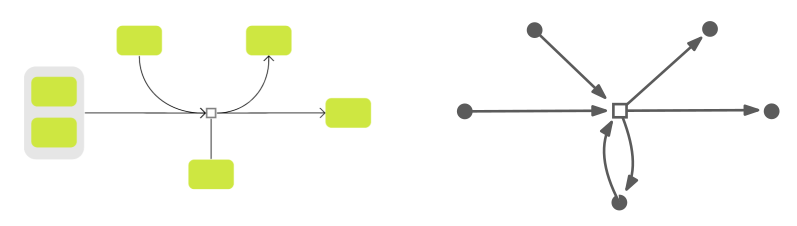
\includegraphics[width=0.7\linewidth]{graph-interpretation.png}
  \caption[Illustration how a rich SBML model is interpreted as a
  graph.]{Illustration of how a rich SBML model is interpreted as bipartite,
    directed graph. The left graphic describes the given \toolname{CellDesigner}-SBML model. Green
    boxes represent species aliases, small white boxes represent reactions.
    Complexes of species aliases are represented by gray boxes. A species alias
    can be involved in a reaction through different kinds of relationship: As
    primary input or output (laid out horizontally to the reaction), as
    secondary in- or output (indicated by curved arcs) or as byproduct without
    directionality (laid out directly below the reaction)}
  \label{fig:graph-construction}
\end{figure}
% TODO extend with example for bipartite projection

% \begin{figure}[h]
%   \centering
%   \begin{subfigure}{0.45\linewidth}
%     % TODO diagram illustrating graph construction: combine drawing of SBML
%     % with simplified graph structure
%     (graph-interpretation) from paper notes
%     \caption{Illustration of how a rich SBML model is interpreted as a simple,
%       directed graph.}
%   \end{subfigure}
%   \begin{subfigure}{0.45\linewidth}
%     todo: something illustrating CellDesigner-SBML structure / distinction between species
%     and species aliases -- or not at all? not really super relevant...
%   \end{subfigure}
%   \label{fig:graph-interpretation}
% \end{figure}


A species alias can either be simple or \ild{complex} in the sense that it
represents a container for other species aliases. This is used to represent e.g.
biological complexes of proteins. Simple and complex species aliases are
arranged in an arbitrarily nested hierarchy. For the graph structure, we
consider only top-level elements, that is, we consider complex species aliases
as single nodes and omit their contents. Contents of complex species aliases
will be taken into account when considering GO annotations
(\refsec{feature-selection}). A reaction may involve an entire complex species
alias (CSA) or only a species alias contained in the CSA. Since we interpret the
CSA as a single node, an edge will be attached to it in either case.

Species aliases can also be contained in \ild{compartments} representing
biological cellular compartments or broader notions of spatial relationship. We
do not consider compartments at all herein (see \refsec{future-work}).

% Attributes such as the species class or the position of the species alias in the
% layout are extracted from the source file and attached as node at

% TODO include diagram of CellDesigner-SBML from miro board?
% ... or anything else illustrating the complexity...



\subsection{Determining ground-truth Labels}
\label{sec:determining-labels}

In order to train any supervised classifier, we require a set of examples for
which the class is already known. Although several disease maps are publicly
available, to the best of our knowledge, none are explicitly annotated with a
per-alias label. Thus, in order to obtain usable training data, we first have to
infer such class labels. Concretely, given a single disease map or a sequence of
reorganisation steps, we need to determine which species aliases are duplicates.

The determination of ground-truth labels is based on comparing a disease map to
a next curation step. Concretely, given maps $D_1$ and $D_2$, and $D_2$ is
created from $D_1$ through some reorganisation, we can infer ground-truth
labels for $D_1$ (but not for $D_2$). See \refsec{determining-labels} for details.

A Disease Map can be given in two different variants. On the one hand, we may be
given a sequence of reorganisation steps of a Disease Map, i.e. a series of intermediate
snapshots of a Disease Map taken during manual curation. On the other hand, we
may simply consider a single, fully laid-out Disease Map.
% TODO check cap of Disease Map

In case we consider a single Disease Map $D$ and not a reorganisation sequence,
we interpret $D$ as the result of some reorganisation. However, as input for a
classifier we actually require the ``previous'' step before reorganisation.
Since this is not explicitly given, we construct a \ild{collapsed} version $D_0$
of $D$ by merging all species aliases that correspond to the same species into a
single representative alias.

\paragraph{Handling reorganisation sequences}
In case we are given a reorganisation sequence, we interpret each snapshot as a
single graph. Since the determination of ground-truth labels is based on the
next graph in the sequence, a given sequence $(D_1, ..., D_k)$ of disease maps
results in a sequence of graphs $(G_0, ..., G_{k-1})$, where $G_i$ is the graph
interpretation of $D_i$. Additionally, $G_0$ is the graph corresponding to the
collapsed version of $D_1$.
% TODO this means the entire experiment on importance of reorganisation steps
% may be weird since it also includes step G_0 -> G_1 which may already be most.
% Let's exclude that and try again. Would then be at least a nice finding.


\paragraph{Determining duplication} Given two graphs $G_t$ and $G_{t+1}$, we
want to infer which species aliases were duplicated in the step from $G_t$ to
$G_{t+1}$. Note that we do not want to identify nodes in $G_{t+1}$ that were
duplicated, but nodes in $G_t$ that will be duplicated. We refer to these as
\ild{duplication parents}. In case we are given a sequence of reorganisation
steps $(G_1, ..., G_k)$ , we infer node labels by comparing successive steps
$G_t$ and $G_{t+1}$. In
% TODO % define reorganisation steps
case we are given only a single disease map $G$, we first construct a collapsed
version $G_0$ by collapsing any species aliases
% TODO calling this G is fishy
corresponding to the same species into a representative node and moving any edges
incident to aliases to the corresponding representative. We then proceed by
comparing $G_0$ and $G$ like reorganisation steps.
%
To make our results comparable to the work of
\citeauthor{nielsen_MachineLearningSupport_2019}
\cite{nielsen_MachineLearningSupport_2019}, we employ the same algorithm for
inferring ground-truth labels. Because the algorithm has received little
explicit treatment in the original publication, we motivate and describe it here
in detail for clarity.
%
% % We motivate the algorithm by first outlining requirements to a procedure for
% % detecing duplicated aliases.
% \begin{itemize}
% \item The case in which merely a copy of a node is introduced and edges are
%   re-attached should also be captured. 
%   % algorithm adresses this by fact that copy will find its duplication parent
%   % (carried over parent will not)
% \item A subgraph reorganisation may include a valid duplication even if an
%   adjacent edge has been removed
%   % adressed by considering to-from/from-to neighbours instead of covering
%   % (ex-remove-edge)
% \end{itemize}
% % TODO does not make much sense to include this list if there are only two
% % points. Its basically saying the same thing as in the sentence above.

A simple approach to identify duplication parents that comes to mind is to
consider nodes newly introduced in $G_{t+1}$ and look for a subset $W \subset
V(G_{t+1})$ whose neighbourhood completely covers the neighbourhood of some node
in $G_{t}$, i.e. $\bigcup_{w \in W} \mathcal{N}_{t+1}(w) = \mathcal{N}_t(v)$ for
some $v \in G_{t+1}$. However, this does not suffice. It is important to note
that we can make no assumptions about what manipulations were made to create
$G_{t+1}$ from $G_t$. In particular, nodes may have been removed, added or
duplicated and edges may have been added, removed or re-wired.
%
To deal with this, instead of finding the duplicates of a given node in
$G_{t}$, the algorithm of \nielsen{} seeks to identify a possible \ild{duplication parent} of
a given node in $G_{t+1}$. The basic idea is that the neighbourhood of
duplicates will be at least partially included in the neighbourhood of the
duplication parent.

Intuitively, the algorithm works by starting at a given node $v_i \in
V(G_{t+1})$, identifying its neighbour nodes in $G_{t+1}$ and considering their
neighbours in $G_t$. If $v_i$ is a duplicate, we expect its duplication parent
to be among these nodes.
% TODO mention that the alg also captures cases where a copy is introduced and
% existing node is kept (in that case the parent will be identified when
% considering the newly introduced node.)

\begin{algorithm}[h]
  \DontPrintSemicolon
  \label{alg:identify-duplicates}
  \caption{ Procedure to identify duplication parents. Transcribed from
    \citeauthor{nielsen_MachineLearningSupport_2019} \cite{nielsen_MachineLearningSupport_2019}.
  }
  \setstretch{1.2} \KwData{Directed graphs $G_t$ and $G_{t+1}$ (reorganisation
    step), node $v_i \in G_{t+1}$} \KwResult{Duplication parent of $v_i$ or
    None} $W_+ \gets \neighb_t^- ( \neighb_{t+1}^+(v_i) )$ \; $P_+ \gets
  \neighb_{t+1}^- ( \neighb_{t+1}^+(v_i) ) \backslash~ W_+$ \; $W_- \gets
  \neighb_t^+ ( \neighb_{t+1}^-(v_i) ) $ \; $P_- \gets \neighb_{t+1}^+ (
  \neighb_{t+1}^-(v_i) ) ~\backslash~ W_- $\;
    %
    \eIf{$W_+ = \emptyset \lor W_- = \emptyset$}{
      $P \gets P_+ \cup P_-$
      \label{line:ambig-cup}
      \;
    }{
      $P \gets P_+ \cap P_-$
      \label{line:ambig-cap}
      \;
    } 
    \eIf{
      $\ensuremath{\norm{P}} = 1$
      \label{line:p-1-check}
    }{
      Let $w$ be the single element in $P$ \;
      \Return $w$ \;
    }{
      \Return None
    }
\end{algorithm}
% TODO what kind of ID? alias ID?
% TODO terminology aliases vs graph nodes

The procedure is given in pseudocode in \ref{alg:identify-duplicates}. For
directed graphs, let the \ild{positive neighbourhood} of $v$ in $G_k$
$\neighb_k^+(v)$ be given as $\{w ~|~ (v,w) \in E(G_{k})\}$ and the \ild{negative
  neighbourhood} $\neighb_k^-(v)$ as $\{w ~|~ (w,v) \in E(G_k)\}$. We abuse set
notation to identify nodes solely based on their alias ID. This means that
$V(G_t)$ and $V(G_{t+1})$ may potentially have nonempty intersection (indeed,
the algorithm relies on it).

Line \ref{line:ambig-cap} states that a valid duplication parent must be
reachable from both positive and negative direction. This is only relevant if
there is no positive (resp. negative) neighbourhood shared between the
reorganisation steps. This is also the case if the target node is a sink, 
respectively source. Line \ref{line:ambig-cup} takes this into account. Then, a
duplication parent may still be uniquely identified if there is a single shared
neighbour in the opposite direction.
% (see \reffig{fig:ex-no-neighb}).
Line \ref{line:p-1-check} handles cases when multiple candidate duplication
parents exist and we cannot infer a unique single one.
% (see example \reffig{fig:ex-p-1}).
The algorithm is able to identify duplication parents even if edges have been
removed.
% (see example \reffig{fig:ex-remove-edge}).



% TODO maybe later, drawing these cleanly is *so* much effort
% \begin{figure}[h]
%   \centering
%   \begin{subfigure}{0.23\textwidth}
%     subfig
%     \caption{Example in which there is no shared positive neighbourhood.
%       However, a unique duplication parent can still be identified because node
%       2 has unit out-degree.}
%     \label{fig:ex-no-neighb}
%   \end{subfigure}
%   \begin{subfigure}{0.23\textwidth}
%     subfig
%     \caption{Example where a unique duplication parent cannot be identified
%       due to ambiguity.}
%     \label{fig:ex-p-1}
%   \end{subfigure}
%   \begin{subfigure}{0.23\textwidth}
%     subfig
%     \caption{Parents can still be inferred if edges are removed. Without node 7,
%     however, the case would be ambiguous}
%     \label{fig:ex-remove-edge}
%   \end{subfigure}
%   \begin{subfigure}{0.23\textwidth}
%     subfig
%     \caption{Ambiguities are resolved by considering both positive and negative
%       neighbourhoods.}
%     \label{fig:ex-ambig1}
%   \end{subfigure}
%   \caption{Examples for Algorithm \ref{alg:identify-duplicates}}
%   \label{fig:alg-examples}
% \end{figure}


\subsection{Data Selection}

% TODO motivation on this

Like \nielsen{}, we exclude complex species aliases and nodes of degree less than
two from prediction. This means they will not be considered as input examples
when training or evaluating the classifier. Note that these nodes are still part
of $G$ and potentially influence the features of other nodes. Further, excluded
nodes will still participate in the message-passing steps of GNN models.

If we are given a sequence of reorganisation steps and duplication events could
be determined in some step, then the graph corresponding to that reorganisation
step contains no nodes with positive labels. In that case, the graph is omitted
from the sequence. 

The set of constructed input graphs is partitioned into training and
testing graphs. For the concrete choice of training and testing partitions, we
explore different settings (see \refsec{experiments-results}).




\subsection{Feature Engineering}
\label{sec:feature-selection}

We are given one or several disease map diagrams and want to make a prediction
for the contained species aliases whether they should be duplicated or not.
Since a graph node, i.e. a species alias, is an abstract mathematical object, we
need to find a representation (description) of a species alias to be used as
input to the classifier. Naturally, the representation should express the
characteristics of the species alias that are relevant to its class.
% Designing such a representation is called \ild{feature engineering}.
Classifiers such as SVMs and NNs commonly expect their input in the form of a
numerical vector.
%
In the following, we define several \ild{features}, \ie characteristics of
species aliases. Such a characteristic can be a vector of numbers or a single
number, in which case we consider it as a one-element vector. Once all
features are computed, their resulting vectors are concatenated into a
single \ild{feature vector} and provided to the classifier as input.

% General remarks on possible features
In general, there are three aspects of a disease map based on which features
can be defined. The first is the \ild{structural} aspect in which we use
graph-theoretical measures to characterise species aliases (graph nodes) based
on their connectivity in the network. This was considered in detail in the
feature engineering step in the work of
\citeauthor{nielsen_MachineLearningSupport_2019}~\cite{nielsen_MachineLearningSupport_2019}
and was used in numerous
approaches for metabolic networks (see \refsec{related-work}).

The second aspect is \ild{semantic}: species are annotated with biological
domain knowledge, commonly in the form of links to databases that provide
additional information about that species (see \refsec{background}). In
this work, we aim to explore how to exploit Gene Ontology term annotations.

The third aspect is that of \ild{layout}: Prior to making a prediction on node
duplication, the disease map may already have been laid out to some extent.
If so, positions of species aliases certainly carry some meaning. Which exactly,
however, is unclear since positions are most likely determined by a mixture of
layout requirements, semantic arrangement and preference of the curator.
%
For the scope of this work, we avoid using layout-based predictors
% TODO mention term predictor in background
since we only have one practical instance in which we have layout information
and ground-truth labels available, which is when making a prediction for a
\dataname{AlzPathway} reorganisation step and comparing it to the actual next
step in the reorganisation sequence. However, this is the only disease map for
which reorganisation steps are available and it is of limited size. Thus we
decide to omit this approach for now, while acknowledging that considering
layout information may lead to interesting approaches (see
\refsec{future-work}). We do consider layout information as a
criterion for attaching edges to duplicates, see \refsec{edge attachment}. 


\paragraph{Structural Features} The following structural features were defined
and used by \citeauthor{nielsen_MachineLearningSupport_2019}~\cite{nielsen_MachineLearningSupport_2019}
. We re-implement
them for comparability. Let $\sigma_{st}(v)$ denote the number of shortest paths
from $s$ to $t$ passing through $v$. Let $\sigma_{st}$ be the number of all shortest
paths from $s$ to $t$. Since in the following, we always consider the graph to
be undirected, $\sigma$ is symmetric.

\begin{itemize}
\item \featname{degree}: The degree of a node, counting both incoming and
  outgoing edges.
\item \featname{clustering_coefficient}: The \ild{clustering coefficient}
  \cite{brandes_NetworkAnalysisMethodological_2005}
  for a
  node $v$ is given as
  \begin{align*}
    \frac{2 \tau(v)}{\deg(v)(\deg(v)-1)}
  \end{align*}
  where $\tau(v)$ is the number of possible triangles through $v$ in the graph.
\item \featname{betweenness_centrality}: The \ild{betweenness centrality} of $v$
  reflects the number of shortest paths that pass through $v$:
  \begin{align*}
    & \sum_{s \not= v} \sum_{t \not= v} \frac{\sigma_{st}(v)}{\sigma_{st}}
  \end{align*}
\item \featname{closeness_centrality}: As used here, the \ild{closeness
    centrality} for $v$ is given by
  % There are different ways to define a
  % closeness-based centrality measure. The definition used here is:
  \begin{align*}
    \frac{\norm{V}-1}{\sum_{s \not= v \in V} d(s,v)}
  \end{align*}
  where $d(s,v)$ is the shortest-path distance from $s$ to $v$.
\item \featname{eigenvector_centrality}: The \ild{eigenvector} centrality is a
  measure of transitive importance of a node. The basic idea is that a node is
  important if it is linked to other important nodes. The centrality values of
  each node are given by the components of the principal eigenvector of the graph's
  adjacency matrix.
\end{itemize}

Additionally, in order to capture the characteristics of a node's direct
neighbourhood, the following secondary features are computed:
\begin{itemize}
\item \featname{neighbour_centrality_statistics}: For node $v$, this is the stacked
  vector of statistics over several centrality measures of neighbours of $v$.
  The statistics are mean, minimum, maximum and standard deviation. The
  centralities are betweenness, closeness centrality, eigenvector centrality and degree.
\item \featname{distance_set_sizes}: A vector of length $k$ in which the $k$-th
  entry is the normalised number of nodes exactly $k$ hops from $v$. Here, $k=5$
  is considered. The values are normalised by the number of nodes reachable in a
  grid graph via $k$ hops.
\end{itemize}

Except for the clustering coefficient, all characteristics are also
computed on the bipartite projection and included as separate features.
Except for \featname{distance_set_sizes}, all features are min-max-normalised
with respect to all given training graphs.

% construction of bipartite projection is based on undirected graph
% centralities are based on undirected graph

Additionally, we consider the directed degrees (\featname{in_degree},
\featname{out_degree}). This is motivated by the notion that a species alias may
have a different biological meaning with respect to node duplication if either in- our
% TODO biological good word to use here?
out-degree is higher, both are balanced or the node is a source or a sink.
% TODO this is repeating to what we write in the results, where to leave it?
% generally think the distance may be bit large and this section has a too fuzzy
% distinction between nielsen features and our thoughts
% TODO this is repeating to what we write in the results, where to leave it?
% generally think the distance may be bit large and this section has a too fuzzy
% distinction between nielsen features and our thoughts




\paragraph{Semantic Features}

A simple semantic feature that \citeauthor{nielsen_MachineLearningSupport_2019}
propose is the one-hot encoding the species type.
The \ild{one-hot encoding} of a categorical variable with $d$ possible values is
a $d$-dimensional binary vector in which $d_i = 1$ if the categorical variable has
value $i$ and $0$ otherwise.
Possible species types are
\textit{protein}, \textit{RNA}, \textit{simple molecule}, \textit{ion},
\textit{gene}, \textit{phenotype}, \textit{drug}, \textit{complex},
\textit{degraded} and \textit{unknown}. 


In addition, we explore using Gene Ontology term annotations to infer meaningful
features.
% We extract GO annotations directly from the given \toolname{CellDesigner}-SBML
% files (see \refsec{gene-ontology-annotations}).
% Given a set of GO term annotations for a species alias, we have to derive a
% fixed-length numeric vector from them that can be used as a feature vector.
%
For a set of GO term annotations, we derive a fixed-length numeric
\ild{embedding} vector for each GO term that reflects its position in the GO
ontology graph, and thus its semantics. We acknowledge that there is previous
work developing pairwise similarity measures between GO terms (see
\nameref{sec:related-work}). However, the direct, embedding-based approach has
the following advantages:
%
\begin{itemize}
\item We are alleviated of the choice of a similarity measure
  (effectively leaving that problem to the classifier). This also means that,
  particularly in case of a GNN classifier, the neural network may potentially
  be able to capture more flexible relationships than what we would encode with
  some similarity measure.
\item This gives us an approach for including annotation information for
  complex species aliases by simply combining the embeddings of contained nodes.
\item Since in the end we aim to assess the heterogeneity of a node's
  neighbourhood, the consideration of embedding values could be incorporated in
  the message-passing step of a neural network (see \nameref{sec:future-work}). Further,
  node-level information may be useful for the task of finding an attachment of
  edges after duplication.
\end{itemize}

% TODO describe node2vec in background?
For computing an embedding vector for a given GO term, we closely follow the
approach of \citeauthor{zhong_GO2VecTransformingGO_2020}
\cite{zhong_GO2VecTransformingGO_2020} and encode a term's position in the GO
graph using the \toolname{node2vec} algorithm.

The above considerations lead to the following concrete feature definitions:
\begin{itemize}
\item \featname{GO_embedding}: The basic idea of this approach is to only provide an
  encoding of the term's position in the GO graph as node feature. A GNN model
  could then potentially capture characteristics of a target node's
  neighbourhood via its aggregation function.
  % TODO move sentences around, we are basically already describing all of this above
\item \featname{GO_stddev}: We additionally try capturing neighbourhood
  heterogeneity by interpreting the embeddings as points in an euclidean space
  and deriving a measure for the spread of these points around their centroid
  (mean). The idea is inspired by the measure of standard deviation, i.e. the
  average squared distance from the mean. This can conventienly be expressed as
  the sum of variances over each dimension. Let $(\vec x_1, ..., \vec x_n)$ be
  the embeddings of neighbour nodes, and let $\bar{\vec x}$ be the centroid
  (i.e. dimension-wise mean). Assume the points lie in a $D$-dimensional
  euclidean space. Let $(\vec x_i)_k$ denote the $k$-th entry of $\vec x_i$. We
  then consider $\sigma = \sqrt{\sigma^2}$ as a measure of spread, given by
  \begin{align*}
    \sigma^2 &= \nicefrac{1}{n} \sum_{i=1}^n \norm{\bar{\vec x} - \vec x_i}_2^2 \\
             &= \sum_{d=1}^D \nicefrac{1}{n} \sum_{i=1}^n
               (\bar{\vec x})_d - (\bar{\vec x_i})_d)^2 \\
             &= \sum_{d=1}^D \text{Var}(\left[
               (\vec x_1)_d, ..., (\vec x_n)_d
               \right])
  \end{align*}
  where $\text{Var}(\left[(\vec x_1)_d, ..., (\vec x_n)_d \right])$ is the
  variance along dimension $d$ and $\norm{\cdot}_2$ is the euclidean distance.
  Note that this approach encodes characteristics of the embeddings across a
  node's neighbourhood directly into a single feature vector and can thus be
  used with any classifier such as SVMs.
  % TODO cite S/O discussion
\end{itemize}


There are two cases when we are required to
aggregate a set of embeddings into a single value. On the one hand, a single
protein can be annotated with several GO terms. On the other hand, a complex
species alias potentially contains muliple annotated aliases. In both cases,
we take the mean of the embeddings associated to the GO terms.


% - compute embedding for each GO term* via node2vec in the GO graph
% note: embedding could also have been computed with GNN method (node
% attributes? positional encoding?) or even integrated in same differentiable
% pipeline. -- but stick to simplicity, has the advantage that embs can be precomputed
% ...- use these as features directly, for complexes take average over all
% contained (GO embedding)
% ...- compute stddev over neighbourhood to directly capture 'diversity'
% * mentioned in the DM


\section{Evaluation of classifiers}
% TODO move this to methods (pretty sure we should)

SVMs as well as GNNs are trained to optimise some specific function with respect
to the training data. However, when comparing and selecting models, we need an
unbiased performance measure that is based only on data and ground-truth labels.

\paragraph{Evaluation metrics} The classifiers considered here will output a
probability (or \ild{confidence score}) that a given data point will belong to
the positive class. To obtain a concrete, binary classification, we have to draw
a \ild{decision threshold} $\tau$. If the predicted confidence score of a given
data point is greater than $\tau$, it will be assigned the positive class, else
the negative class.
%
In \reftab{conf-names} we introduce some basic terminology for subsets of
training data based on their true and predicted class
\cite{tharwat_ClassificationAssessmentMethods_2021}.
\begin{table}[h]
  \centering
  \begin{tabular}[h]{l | l l}
    & Predicted Positive (\PP{}) & Predicted Negative (\PN{}) \\
    \hline
    Actually Positive (\P{}) & \ild{True Positives} (\TP{}) & \ild{False Negatives} (\FN{}) \\
    Actually Negative (\N{}) & \ild{False Positives} (\FP{}) & \ild{True Negatives} (\TN{})
  \end{tabular}
  \caption{Given a concrete, binary classification, the following terms describe
  (sizes of) subsets of the predicted data, depending on its ground-truth and predicted class.}
  \label{tab:conf-names}
\end{table}
% TODO formatting (space after command)

Based on the terms in \reftab{conf-names}, we define the following measures:
% TODO reference for this
\begin{itemize}
\item \ild{Accuracy}, given by the ratio of
  correctly classified examples: $\nicefrac{\TP{} + \TN{}}{\P{}+\N{}}$. Note that for
  class-imbalanced data, this is not a sufficient measure, because
  misclassifications of the minority class will be underrepresented in the
  overall score.
\item  \ild{True Positive Rate} (\TPR{}), or \ild{Recall}, given by $\nicefrac{\TP{}}{\P{}}$ is
  the probability that a positive example will be predicted as such by the classifier.
\item \ild{False Positive Rate} (\FPR{}), given by $\nicefrac{\FP{}}{\N{}}$ is the
  probability that a negative example will be predicted falsely as positive.
  \item \ild{Precision}, given by $\nicefrac{\TP{}}{\PP{}} = 1 - \FPR{}$
\end{itemize}

A perfect classifier would yield a high True Positive Rate and a low False
Positive Rate.
%
Note that it is possible to trade-off \FPR{} and \TPR{}
by varying the decision threshold. If the threshold is very high, only examples
for which the classifier has high confidence will be actually assigned positive
class. This means that the \FPR{} will be low. However, then not all true
positives may be picked up as such by the classifier, resulting in a low \TPR{}.
Lowering the decision threshold will increase \TPR{}, but also potentially result
in additionally picking up false positives, increasing the \FPR{}.

The choice of the proper decision threshold
% i.e. the tradeoff between Recall
% and Precision
depends on the use-case since different importance may be assigned
to either Precision or Recall.
%
The original use-case of \nielsen{} was to use a classifier trained for predicting
% TODO space after command
node duplication to provide a low number of high-confidence examples as
suggestions to the user. When considering only the few examples with the highest
score, Precision is more important than Recall.

To assess the trade-off between \FPR{} and \TPR{} with respect to possible choices of
classification threshold $\tau$, we can plot \FPR{} and \TPR{} as a function of
$\tau$, yielding the \ild{Receiver Operating Characteristic} (ROC curve). The
curve of a random classifier that flips an even coin for each given example would
be close to the diagonal. 
%
Generally, a classifier could be considered better if its ROC curve leans
towards the upper left, i.e. the area under the curve is greater.

As a heuristic for choosing $\tau$, we can look for the threshold with the greatest
distance between \TPR and \FPR at $\tau$, i.e. $\tau_{\text{opt}} := \argmax_{\tau \in
  (0,1)} \TPR{}(\tau) - \FPR{}(\tau)$.
As an indicator for overall quality, we can compute the \ild{Area Under Curve}
(AUC) score given as
\begin{align*}
  \text{AUC}(\tau) = \nicefrac{1}{2} (\TPR{}(\tau) - \FPR{}(\tau) + 1)
\end{align*}
and define the optimal overall AUC score as $\text{AUC} := \text{AUC}(\tau_{\text{opt}})$.
However, we acknowledge that reducing the performance of a classifier to a
single number will hardly ever capture all characteristics and evaluation still
depends heavily on the use-case.


% TODO rephrase this sentence
\paragraph{On evaluation of NNs} To avoid overfitting, for overall performance
evaluation, we consider the model state at the training epoch that performs best
on the validation split. This is not necessarily the best epoch with respect to
the training split, see \reffig{fig:svm-repro-loss}. The tradeoff can also be
seen in shape of imperfect performance on the training split in the ROC curves.
% 
% TODO terminology: split
%
Note that, in practise, a ML model should be able to reliably generalise to data
that was not observed during the process of finding and tuning a model. Usually,
this is done by splitting the available data into three parts: one for training,
one for evaluation during model tuning (such as identifying a reasonable maximum
epoch like here) and, finally, a part that will only be used for validation once
all decisions have been made, to assess the actual generalisation performance of
the final model.
%
Here, we are technically still in the first stage. In the future, potentially,
once a single, promising model has been identified and all decisions have been
made, there must be anothe validation on completely unseen data.

\section{Attachment of edges}
\label{sec:edge-attachment}


Assume we are given a binary classifier that decides whether a node should be
duplicated. If a node $v$ is eligible for duplication, we next need to determine
how many duplicates to introduce and how to distribute edges to and from $v$
across the duplicates. Formally, we aim to find a partition of the neighbourhood
of $v$. Based on the intuition that a good duplication is one that reduces the
heterogeneity of the neighbourhood, we can characterise the partitions as
\ild{clusters} in the sense that intra-cluster distances are smaller than
inter-cluster distances.

The choice of distance metric is open. Of particular interest are metrics that
reflect semantic similarity of attached GO terms
(see \nameref{sec:related-work}).
% \footnote{ Indeed,
%   \citeauthor{ostaszewski_ClusteringApproachesVisual_2018} applied GO semantic
%   similarity to cluster nodes in a disease map. }
However, because in the given
datasets, most aliases are annotated with a relatively large number of GO terms
and exploiting these annotations for classification was problematic (see \nameref{sec:experiments-results}),
% did not yield gains in
% classification performance most likely due to high ambiguity,
we opt for a
simpler approach first and leave this open to future work. 
Instead, we consider the layout positions of aliases and their euclidean
distances. Note that this approach is only applicable if layout information is
actually given, i.e. this approach can not be used if we construct a collapsed
graph from a single given disease map (unless we would infer layout information
for the newly constructed, collapsed graph).

Particularly when considering euclidean distances in the layout, a suitable
clustering algorithm needs to handle outliers in a sensible manner.
Additionally, we do not know the number of clusters in advance. This eliminates
basic partition-based methods such as $k$-\textsc{Means} and extensions.
%
Further, we seek to assign all points to a cluster, i.e. we do not want to
exclude any points as noise. Also, since different node neighbourhoods have
potentially different scales, we aim to avoid having to specify hyperparameters
like distance thresholds as they are used in density-based clustering algorithms
like \textsc{DBSCAN} or \textsc{Optics}.
%
A family of clustering algorithms that seems well suited is that of
\ild{agglomerative} clustering: Initially, each point is assigned its own
cluster. Iteratively, the two clusters with the smallest inter-cluster-distance
are merged until only a single cluster remains. This yiels a hierarchical
clustering tree, also called \ild{dendrogram}, as depicted in
\reffig{neighb-clust-examples}.

There are several canonical choices of distance measures between two clusters $C_1$ and
$C_2$. The most simple ones employed for agglomerative clustering are:
\begin{align*}
  \text{\ild{single linkage:}} &~~ d(C_1, C_2) = \min_{p \in C_1, q \in C_2} d(p,q) \\
  \text{\ild{complete linkage:}} &~~ d(C_1, C_2) = \max_{p \in C_1, q \in C_2} d(p,q) \\
  \text{\ild{centroid linkage:}} &~~ d(C_1, C_2) = d(\text{mean}(C_1),\text{mean}(C_2))
\end{align*}
where $C_1$ and $C_2$ are considered to be sets of points. Complete linkage and
centroid linkage seem inadequate since they would be strongly affected by large
in-cluster variances and do not work well if clusters are not convex.
% and do not work well if clusters not convex

Setting a threshold value on the maximum dissimilarity inside a cluster, we
obtain a concrete clustering. This can be thought of as ``cutting off'' the
dendrogram at a specific height. Note that here we do not have to specify the
number of clusters but instead a threshold dissimilarity. This threshold can be
determined automatically via a heuristic:
% \footnote{
%   This is basically the \ild{elbow method} in which we plot clustering quality
%   % TODO citation?
%   against number of clusters and aim to find an elbow (i.e. bend) in the curve.
%   Clustering quality here would be the minimum inter-cluster distance of two yet
%   unmerged clusters.
% }
We look for the strongest increase in the distance to
the next closest cluster before each merge step. Formally, let $d = (d_1, ..., d_k)$
be the monotonically increasing sequence of inter-cluster distances at which a
merge occured. The first discrete derivative $d'$ of this sequence gives the step
sizes while the second derivative $d''$ describes the change rate in step sizes. The
index of the maximum in $d''$ yields the number of clusters.
Note that we require $k \geq 8$ points for determining at least two values in the second
discrete derivative. In case of $k < 8$, we fall back to the first derivative
(step size). Examples show that this is a good approximation for a low number of points.
%
As special cases, since the decision to duplicate is assumed to be already given
by the classifier, we exclude the possibility of returning only a single
cluster. If $\norm{\neighb(v)}=2$, then we always trivially split. 

Note that thus we characterise the procedure to identify the number of clusters
independently of the concrete scale of the data. However,
we can see that this procedure strugges if
intra-cluster variances are diverse an the internal variance of a
cluster is close to another inter-cluster distance (see \reffig{neighb-clust-examples}).
We accept this disadvantage
for now and hypothesize it has little practical impact in this use-case.



\section{Implementation}

The experiments in this work were realised mainly using Python. For deep
learning on graphs, we use the library \toolname{PyTorch Geometric}
\cite{fey_FastGraphRepresentation_2019}
which
provides implementations for most popular message-passing layers. It is based on
the deep learning framework \toolname{PyTorch}
\cite{paszke_PyTorchImperativeStyle_2019}. We use the SVM implementation
provided by \toolname{scikit-learn}
\cite{pedregosa_ScikitlearnMachineLearning_}.

Data preprocessing such as loading from SBML files, constructing the graph and
identifying duplicates was mostly done in standard Python using core libraries.

For the computation of structural features, we used either \toolname{networkx}
\cite{hagberg_ExploringNetworkStructure_2008}
or the Python frontend of \toolname{igraph}
\cite{csardi_IgraphSoftwarePackage_}
if computation speed was relevant.
Because the input networks are of nontrivial size (see \refsec{datasets-used}),
computation time has to be taken into account.
Particularly attributes relying on global information (such as e.g. closeness
centrality) can provide a challenge for high-level graph libraries such as
\toolname{networkx} and may not be computable in a reasonable amount of time. More
sophisticated implementations working with a lower-level language such as those
provided by the \toolname{igraph} library used herein show a significant speedup.

The pipeline of preprocessing and model training is based on \toolname{GraphGym}
\cite{noauthor_snap-stanfordgraphgym_2021}, an open-source project that offers a
modular pipeline for deep learning on graphs. It was initially developed for
exploring the design space of GNNs \cite{you_design_2020}. We extend
\toolname{GraphGym} to fit our needs. Some of the main extensions are
\begin{itemize}
\item Having different graph interpretations of a disease map (simple,
  bipartite, directed, undirected, ...) available simultaneously when needed,
  but only computing them when actually required for the current experiment.
\item Handling and converting between different graph data structures such as
  those provided by \toolname{networkx}, \toolname{DeepSNAP} (used internally by
  \toolname{GraphGym}) and \toolname{igraph} (used for fast algorithms on graphs).
\item Avoid splitting provided graphs internally but instead make it possible to
  train on some and evaluate on other (whole) graphs.
\item Caching feature computations so they do not have to be recomputed on each
  experiment run.
\end{itemize}

GO term annotations were extracted and handled using the \toolname{KNIME
  Analytics Platform}
\cite{gesellschaftfurklassifikation_DataAnalysisMachine_2008}
as well as as Python with libraries such as
\toolname{pandas}
\cite{reback_PandasdevPandasPandas_2021}
and \toolname{numpy}
\cite{harris_ArrayProgrammingNumPy_2020}. For the computation of embedding
vectors, we used the \ild{node2vec} implementation provided by \toolname{PyTorch
Geometric}.


% what did I spend time on programming?
% - read data from XML
% - exclusion of individual nodes
% - keeping & managing different graph interpretations (simple, bipartite etc),
% and representations (networkx, igraph, deepsnap, ...)
% - disable internal split
% - feature augments
% - evaluation and comparison of results
% - GO: read, compute, combine, ...


% learning on graphs, GNN:
% PyTorch, PyTorch Geometric, GraphGym, Extensions


% SVM: scikit-learn

% graph representation & computations on graph structure
% 
% \citeauthor{nielsen_MachineLearningSupport_2019} additionally consider the
% centralities of a given node in its ego graphs of sizes $3$ and $5$. Due to time
% constraints, we omit this feature. We note that we achieve comparable
% classification performance as reported the original work even without using that
% feature (see \nameref{sec:experiments-results}).



% ====================================
\chapter{Experiments \& Results}
\label{sec:experiments-results}

We motivate and describe the experiments that were carried out and discuss their
results. We begin with some preliminary models identified via basic
hyperparameter search. Each subsequent section is based on the best-performing
model of the previous section. A discussion from a general viewpoint follows in
\refsec{discussion}. The applied methods and features are described in detail in
\refsec{methods}.

\section{Datasets used for training and evaluation}
\label{sec:datasets-used}

Since disease maps are manually created, the availability of diagrams is
limited.
% should be comparable -- but dont even know w.r.t what
Here, we focus on data already considered in previous work
\cite{nielsen_MachineLearningSupport_2019}. We describe the used disease maps
and provide a visual overview in \reffig{maps-summary}.

The \ild{AlzPathway} map describes signaling pathways related to Alzheimer's
Disease. Since its initial publication~\cite{mizuno_AlzPathwayComprehensiveMap_2012}, it has received several updates
and further analyses~\cite{ogishima_MapAlzheimerDiseasesignaling_2013,
  ogishima_AlzPathwayUpdatedMap_2016, mizuno_NetworkAnalysisComprehensive_2016}.
%
The map has received additional curation focussing on increasing readability by
means of reorganising existing network elements~\cite{ostaszewski_AlzPathwayRegorganisationSteps_2021}. This includes the
duplication of some species aliases. During curation, snapshots of intermediate
progress (\ild{reorganisation steps}) were saved. Note that the reorganisation
steps are not atomic. Each step includes modifications to several nodes and
edges. This sequence of reorganisation steps served as the basis for the work of
\citeauthor{nielsen_MachineLearningSupport_2019} to train an SVM classifier to
predict node duplication \cite{nielsen_MachineLearningSupport_2019}. In this
work, we consider these reorganisaton steps for training data
(\dataname{AlzPathwayReorg}). Note that from the sequence of reorganisation
steps, we exclude the steps that do not correspond to any duplication events.
Further, we consider the last of the reorganisation steps, i.e. the final result
as a single, independent map (\dataname{AlzPathwayReorgLast}). For both
reorganisation steps and fully-curated map, we use the dataset published by
\citeauthor{ostaszewski_AlzPathwayRegorganisationSteps_2021}
\cite{ostaszewski_AlzPathwayRegorganisationSteps_2021}.

The \ild{PDMap} \cite{fujita_IntegratingPathwaysParkinson_2014} describes the
major pathways involved in the pathogenesis of Parkinson's Disease. The map can
be explored via a hosted \toolname{Minerva} instance, reachable at
\url{https://pdmap.uni.lu/minerva}. For this work, we consider the version of
this map as exported from \toolname{Minerva} at 2021-09-07.

\ild{ReconMap}
\cite{noronha_ReconMapInteractiveVisualization_2017}
is a visual representation of the genome-scale metabolic model
\ild{Recon 2} \cite{thiele_CommunitydrivenGlobalReconstruction_2013} that aims
to comprehensively model the human metabolism. It can be viewed at \url{https://vmh.life/minerva}.
We use version \cd{2.01} from 2015-11-20.

\begin{figure}[h]
  \centering
  \begin{subfigure}{0.32\textwidth}
    % ADReorgLast summary
    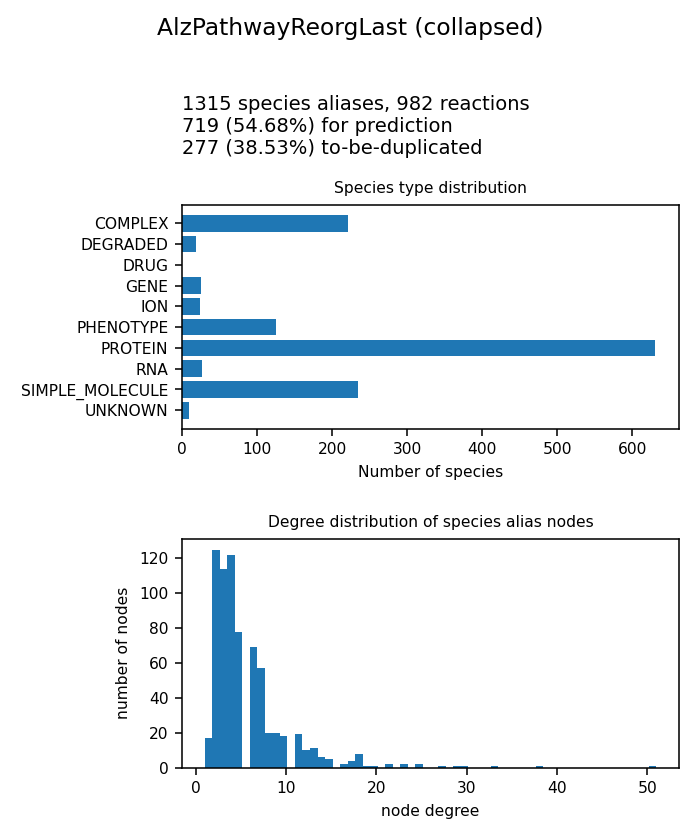
\includegraphics[width=\linewidth]{generated/AlzPathwayReorgLast.png}
  \end{subfigure} 
  \begin{subfigure}{0.32\textwidth}
    % PDMap summary
    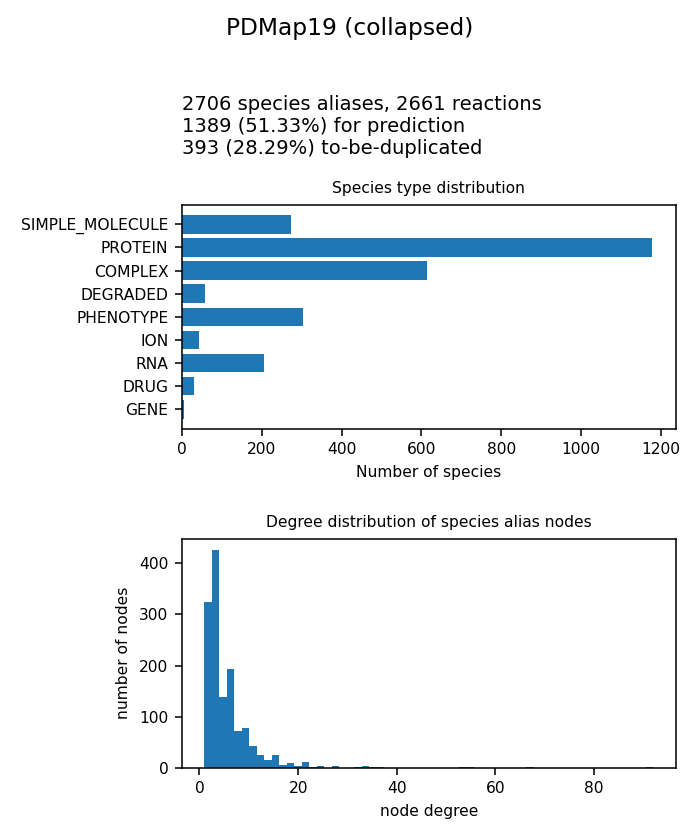
\includegraphics[width=\linewidth]{generated/PDMap19.png}
  \end{subfigure} 
  \begin{subfigure}{0.32\textwidth}
    % ReconMap summary
    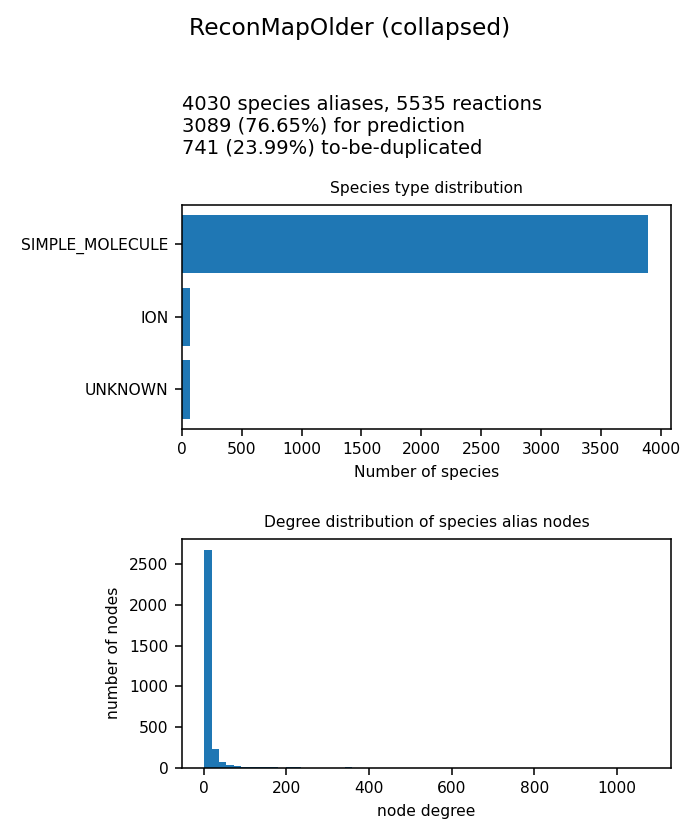
\includegraphics[width=\linewidth]{generated/ReconMapOlder.png}
  \end{subfigure} 
  \caption[
  An overview of characteristics of networks used for training.
  ]{ An overview of characteristics of the \textit{collapsed} networks
    used for training. The count of species aliases and reactions is effectively
    the count of the bipartite node sets in the constructed graphs. Since we are
    consiering collapsed diagrams, the count of species aliases equals the count
    of species.
    Networks and labels are determined as described in
    \refsec{datasets}. }
  \label{fig:maps-summary}
\end{figure}
% TODO consistent ordering of bars!
% TODO assess&remove&mention-explicitly node degree outliers for ReconMapOlder
% to make plot more informative

% TODO mention discrepancy between sequence and collapsed
% TODO using sequence of train and collapsed as validate may be problematic
% because different characteristics?
% particularly reconmap looks quite different?
% cf train-on-many?

% TODO adress concern 'but is it OK to use NN on small dataset'
% by providing examples of comparable work
% by saying that GNNs are potentially of much lower complexity than the computer
% vision NNs you see.

% TODO practical concerns on SVMs:
% - few hyperparams
% - formulation naturally seems suited for little training data
% maybe notes from end of here: https://people.csail.mit.edu/dsontag/courses/ml13/slides/lecture6.pdf
% TODO practical concerns on NNs:
% many hyperparameters that need to be picked/tuned
% convergence not guaranteed
% unique 'solution' not guaranteed
% complex / expensive


In experiments, we will consider different sets of node features as input to the
classifier. We outline these \ild{feature sets} in table
\reftab{feature-importance-feature}. The set \cd{basic-both} is the same set of
features as used by \nielsen{}, with the exception of omitting one particular
feature. For a node $v$, the feature would contain statistics on centrality
scores of $v$'s neighbours in the ego graph centered on $v$ of radius $k$ for $k
\in \{3,5\}$. This feature was not included in preliminary experiments due to
computational cost. This somehwat impacts comparability to the previous work.
However, note that we achieve the same performance even if not using this
feature. This suggests that this feature is not essential here.

\begin{table}[h]
  \small
  \centering
\begin{tabular}[h]{r | c c c c c}
  & \cd{basic-both} & \cd{basic-projection} & \cd{basic-simple} & \cd{degrees} & \cd{degrees-basic} \\
  \hline
  \cd{betweenness_centrality} & \chk & - & \chk & -  & -  \\
  ...\cd{projection} & \chk & \chk & -  & -  & -  \\
  \cd{closeness_centrality} & \chk & -  & \chk & -  &-  \\
  ...\cd{projection} & \chk & \chk & -  & -  & -  \\
  \cd{eigenvector_centrality} & \chk & - & \chk & -  &- \\
  ...\cd{projection} & \chk & \chk & -  & -  & -  \\
  \cd{neighbour_centrality_statistics} & \chk & - & \chk & -  & - \\
  ...\cd{projection}  & \chk  & \chk & - & -  &- \\
  \cd{distance_set_size}  & \chk & \chk  & \chk & - & - \\
  \cd{clustering_coefficient}  & \chk & \chk & \chk & -  &- \\
  \cd{node_class_onehot} & \chk & \chk & \chk & -  &- \\
  \cd{node_degree} & \chk & - & \chk & \chk & \chk \\
  ...\cd{projection} & \chk & \chk & - & \chk & \chk \\
  \cd{node_in_degree} & - & - & -  & \chk & - \\
  \cd{node_out_degree} & - & -  & -  & \chk & - \\
\end{tabular}
  \caption{Overview over the different feature sets.}
  \label{tab:feature-importance-features}
\end{table}


\section{Basic hyperparameter search}
\label{sec:hyperparameter-search}
% cf [[tune or pick hyperparams]]

The models were trained on the AlzPathway reorganisation steps (\ADMap) and
evaluated on the Parkinson's Disease Map (\PDMap). The considered features in
this and subsequent experiments are, unless stated otherwise, based on the work
of \nielsen{} (see \cf{basic-both} in \reftab{feature-importance-features}). We
select the best-performing model with respect to AUC score.

\subsection{Support Vector Machine}
% - svm-repro
% - train-on-many/train-on-many-svm

For the choice of kernel function, we pick the RBF kernel (see
\refeq{rbf-kernel}) as a heuristic choice since
\citeauthor{nielsen_MachineLearningSupport_2019} showed that a generally
best-performing kernel cannot easily be determined and that the RBF
kernel generally achieves good performance.
%
Since we use a different SVM implementation than \nielsen{}, that might
potentially interpret the parameters slightly differently.

Since no previous implementation was publicly available, we may be using a
different SVM implementation that originally applied by \nielsen{}. Different
implementations may interpret parameters slightly differently. Thus, we perform
grid search over a similar range of values to determine a best-performing set of
hyperparameters.

The weight hyperparameter specifies the weight of the minority class. Here, this
is the positive class. It corresponds to the value $C_P$ in \refeq{svm-imbalanced}.

% for the
% choice of \cd{C} and $\gamma$, we additionally perform grid search over the same
% ranges of values.
%
The results are given in \reftab{svm-hyperparams}. The choices of \cd{C},
$\gamma$ and weight roughly agree with the results of \nielsen{}.

\begin{table}[h]
  \begin{tabular}[h]{| l | l | l |}
    \textit{Hyperparameter} & \textit{Searched range} & \textit{Choice} \\
    \hline
    Cost (\cd{C}) & $2^{-9}$ to $2^3$ & 0.5 \\
    Gamma ($\gamma$) & $2^{-3}$ to $2^{9}$ & 0.1 \\
    Weight & \cd{[1,2,3,5,7,10]} & 3
  \end{tabular}
  \caption{Considered SVM hyperparameters, value range searched via grid search and
    best identified combination of values.}
  \label{tab:svm-hyperparams}
\end{table}



\subsection{Graph Neural Network}
% see experiment dirs:
% - gcn-projection was main hyperparam search
% - small-optimisations

The range of searched hyperparameters is based on the work of
\citeauthor{you_design_2020} who systematically evaluated choices of hyperparameters for
various tasks \cite{you_design_2020}. They suggest a constrained design space
for Graph Neural Networks for tasks such as node classification.  

\begin{table}[h]
  \begin{tabular}[h]{| l | l | l |}
    \textit{Hyperparameter} & \textit{Searched range} & \textit{Choice}  \\
    \hline
    Dropout & \cd{[0.0, 0.1,0.2,0.4]} & \cd{0.0} \\
    Aggregation function & \cd{[add, mean, max]} & \cd{add} \\
    Fully-connected layers before message-passing & \cd{[1,2]} & \cd{2}\\
    Fully-connected layers after message-passing & \cd{[2,3]} & \cd{2}\\
    Message-passing layers & \cd{[2,4,6,8]} & \cd{2} \\
    Connectivity & \cd{[skip_sum, skip_cat]} & \cd{skip_sum} \\
    Activation function $\sigma$ & \cd{[PReLU]} &   \\
    Use batch normalisation? & \cd{[yes]} & \\
    Learning rate $\eta$ & \cd{[0.01]} & \\
    % TODO Learning rate decay & \cd{[0.0, *0.1*]} \\
    % TODO weight decay, normalise adj, cf small-optimisations
    Optimiser & \cd{[adam]} & 
  \end{tabular}
  \caption{Considered hyperparameters for the GNN models. In case there are
    multiple possible values, the best hyperparameter combination is given in
    the third column.} 
  \label{tab:gnn-hyperparams}
\end{table}

% TODO elaborate on hidden layer size

% TODO explain dropout, skipsum


\section{Reproducing previous work \& Comparison to GNN}
% svm repro, svm-repro-reconmapolder

In this section, we reproduce the original task from \nielsen{} using an SVM
classifier. Additionally, we introduce a simple GNN classifier based on the
GCN layer defined in \refsec{neural-networks} that operates on
the same input data as the SVM, using the bipartite projection of the disease
map graph for message-passing (see \refsec{graph-interpretation}). Further
variants and extensions of the GNN model will be evaluated in the following
sections.

% TODO move this somewhere else, does not belong in Discussion
The initialisation of neural network weights before the training depend on
random values. To check whether our training procedure is robust with respect to random
initialisation, we repeat each run several times with different seed values for
the random number generators. The separate runs are illustrated as multiple
lines in the figures in this section. Since this seems to be fairly stable, we omit this
in future experiments for sake of simplicity.
% NOTE order of training samples does not matter as we are doing full-batch training

% NOTE taking graphic from repeats experiment here
\begin{figure}[h]
  \centering
  \begin{subfigure}[h]{0.49\linewidth}
    \pic{svm-repro/results/config-svm/roc.png}
    \caption{SVM classifier.}
  \end{subfigure}
  \begin{subfigure}[h]{0.49\linewidth}
    \pic{svm-repro-repeats/results/config-gnn/roc.png}
    \caption{GNN classifier, 5 repeats.  }
  \end{subfigure}
  \caption{ROC Curves for SVM and GNN classifiers trained on \ADMap{}
    and evaluated on the same dataset (\textit{training set}, dashed line) or on \PDMap
    (\textit{testing set}, solid line).}
  \label{fig:svm-repro-comparison}
\end{figure}
%
\begin{figure}[h]
  \centering
  \begin{subfigure}[h]{0.49\linewidth}
    \pic{svm-repro-repeats/results/comparison/roc.png}
    \caption{Comparison of ROC Curves of SVM and GNN classifiers.}
  \end{subfigure}
  \begin{subfigure}[h]{0.49\linewidth}
    \pic{svm-repro-repeats/results/comparison/cutoffs.png}
    \caption{Comparison of \FPR values at specific \TPR cutoff values (lower is better). These
      values are specific points from the ROC curve.}
  \end{subfigure}
  \caption{(\ADMap{} $\rightarrow$ \PDMap) Direct comparison of SVM and GNN classifier. The data
    corresponds to the solid lines in \reffig{svm-repro-comparison}.}
  \label{fig:svm-repro-roc-train-test}
\end{figure}
% TODO coalesce into single figure s.t. they dont split?

% TODO discussion on ROC curves and on cutoffs
% - In general, models able to generalise
% - SVMs and GNNs pretty much the same for high precision, GNNs slightly better
% in the middle
% on cutoffs: compare to what is given in nielsen

\begin{figure}[h]
  \centering
  \begin{subfigure}[h]{0.49\linewidth}
    \pic{svm-repro/results/config-gnn/loss.png}
  \end{subfigure}
  \begin{subfigure}[h]{0.49\linewidth}
    \pic{svm-repro/results/config-gnn/loss-25.png}
  \end{subfigure}
  \caption{Total loss value at each training epoch of the GNN model. The right-hand-side plot a
    focussed view on the same data.}
  \label{fig:svm-repro-loss}
\end{figure}
% TODO discussion on loss value -- maybe actually put this in discussion, since
% this is a thing for all experiments/tasks?
% TODO also show performance on train
% -- will show that already sort of hard to overfit on training data?

% TODO mention that this is an advantage of NNs since it seems to be able to
% handle messy data better?



% NOTE this is for ReconMap
\begin{figure}[h]
  \centering
  \begin{subfigure}[h]{0.49\linewidth}
    \pic{svm-repro-reconmapolder-repeats/results/comparison/roc.png}
    \caption{Comparison of ROC Curves of SVM and GNN classifiers.}
  \end{subfigure}
  \begin{subfigure}[h]{0.49\linewidth}
    \pic{svm-repro-reconmapolder-repeats/results/comparison/cutoffs.png}
    \caption{Comparison of \FPR values at specific \TPR cutoff values (lower is better). These
      values are specific points from the ROC curve.}
  \end{subfigure}
  \caption{(\ADMap{} $\rightarrow$ \ReconMap).
    Direct comparison of SVM and GNN classifier evaluated on \ReconMap{}.}
  \label{fig:svm-repro-reconmapolder-roc-train-test}
\end{figure}
% NOTE this is for ReconMap
\begin{figure}[h]
  \centering
  \begin{subfigure}[h]{0.49\linewidth}
    \pic{svm-repro-reconmapolder/results/config-gnn/loss.png}
  \end{subfigure}
  \begin{subfigure}[h]{0.49\linewidth}
    \pic{svm-repro-reconmapolder/results/config-gnn/loss-25.png}
  \end{subfigure}
  \caption{Total loss value at each training epoch of the GNN model, evaluted on
    \ReconMap{}. The right-hand-side plot a focussed view on the same data.}
  \label{fig:svm-repro-reconmapolder-loss}
\end{figure}



\paragraph{Results \& Discussion}
% comparison to results of nielsen
% PDMap: pretty much the same (see fig. 5 in nielsen)
% Reconmap: slightly worse than reported results but ReconMap is difficult
% anyway and may be due to smaller difference in hyperparams (see fig. 6 in nielsen)
The performance of the SVM model agrees with the evaluation metrics reported by
\nielsen{}. For evaluation on \PDMap, the performance is almost the same. For
evaluation on \ReconMap{}, the performance is only slightly worse. This may be due
to a slightly different choice of hyperparameters in our case.

As a first sanity check for the GNN approach, we verify whether the optimisation
procedure is able to overfit the model on the training data. Indeed, the overall
loss value converges to a stable minimum and the AUC score for evaluation on the
training set at the last epoch is $0.989$, indicating a near-perfect fit (not
shown in figures). Note that in \reffig{svm-repro-comparison}, we instead report
the performance on the training set of the model state that performed best on
the validation set.

For both evaluation on \PDMap and on
\ReconMap{}, the GNN's ROC curve dominates the SVM's curve. This means that for a
given \FPR deemed acceptable, the GNN model will provide a higher ratio of True
Positives. This advantage grows as the decision threshold is lowered, i.e. the
GNN model is better particularly when we aim to identify more than just the
high-confidence examples. The difference between ROC curves is only slight on
evaluation on \PDMap but strong on evaluation on \ReconMap{}. This may be due to a
better ability of the GNN model to generalise, given the different
characteristics of \ReconMap{}.
% TODO can we say more about this now that we know that reorg steps break a lot?

Note how, for both \PDMap and \ReconMap{} as evaluation datasets, the validation
loss reaches its minimum after just a handful of training epochs. We
additionally ran the same experiment with a decreased learning rate ($0.01
\rightarrow 0.001$). There, we can see a smoother decrease the loss value, but
also note that the overall achieved minimum is worse than in case of a greater
learning rate (see \reffig{svm-repro-lowlr-reconmapolder-loss}). This makes it
very questionable, how robust model training actually is in this case if the
same progress cannot be reliable replicated in a greater number of smaller steps.
\begin{figure}[h]
  \centering
  \begin{subfigure}[h]{0.49\linewidth}
    \pic{svm-repro-reconmapolder-lowlr/results/config-gnn/loss.png}
  \end{subfigure}
  \begin{subfigure}[h]{0.49\linewidth}
    \pic{svm-repro-reconmapolder-lowlr/results/config-gnn/loss-100.png}
  \end{subfigure}
  \caption{Total loss development with decreased learning rate. The plot shows
    the total loss value at each training epoch of the GNN model, evaluated on
    \ReconMap{}. The right-hand-side plot a focussed view on the same data.}
  \label{fig:svm-repro-lowlr-reconmapolder-loss}
\end{figure}


\section{Importance of Reorganisation Steps}
Recall that in case of Alzheimer's Disease Map, we are
given a sequence of reorganisation steps. The original approach of \nielsen{} was
train a model on the entire sequence of reorganisation steps s.t. the model
would mimic the actions of a human curator as closely as possible. They would
then evaluate the model on \textit{collapsed} versions of other disease maps.
%
A fully collapsed map potentially has vastly different characteristics than a
partially curated map. For instance, a collapsed map is likely to contain
species aliases of very high degree (maybe those that appeared often as
independent aliases before collapse). In a reorganisation step, on the other
hand, the map will already be in part curated and some nodes already duplicated.
%
So, we might effectively be training our models to do one task while testing
them on a slightly different task.
%
This consideration is also relevant if we consider a slightly different
use-case: one of the first steps in the construction of a disease map may be the
semi-automatic concatenation of different pathways, during which species
appearing in several pathways will be mapped to the same species alias, i.e.
there will be exactly one alias per species. Such a map will very closely
resemble a collapsed map in the sense we construct it here.
%
Additionally, a reorganisation sequence is likely to contain contradictory
examples: An alias that is duplicated only in a later step will appear as
negative example in all previous steps. Further, the concatenation of all
reorganisation steps into one big, disconnected graph for training
% TODO verify that we are indeed doing this and describe it earlier
will further amplify the inherent class imbalance.
%
Thus, we deem it interesting to explore how a model will perform if trained not
on the reorganisation steps but simply the collapsed version of the final map.
%
This has the additional advantage that in practise, reorganisation steps will
rarely be available. The collapsed version, however, can be constructed from any
published disease map.

\begin{figure}[h]
  \centering
  \begin{subfigure}[h]{0.48\linewidth}
    \pic{svm-repro-adlast/results/comparison/roc.png}
    % \pic{svm-repro-adlast/results/}
    % \pic{svm-repro-reconmapolder-lowlr/results/config-gnn/loss.png}
    \caption{(\ADLast $\rightarrow$ \PDMap)}
  \end{subfigure}
  \begin{subfigure}[h]{0.48\linewidth}
    \pic{svm-repro-reconmapolder-adlast/results/comparison/roc.png}
    \caption{(\ADLast $\rightarrow$ \ReconMap{})}
  \end{subfigure}
  \caption{ROC curves of models trained on collapsed version of the
    \textit{AlzPathway} map (not the reorganisation steps).}
  \label{fig:importance-reorganisation-steps}
\end{figure}

\paragraph{Results \& Discussion} The results are illustrated in
\reffig{importance-reorganisation-steps}. Note how both SVM and GNN models do
not degrade noticeably in performance (compare to \reffig{TODO}). In
fact, the SVM model performs \textit{better} when trained on the collapsed map,
potentially due to fewer contradictory examples. The GNN models show similar
performance.

% TODO adress how there is no longer a performance gap between SVM and GNN
% (G)NNs can handle the nasty case better?

Another factor to consider here is that collapsed maps are constructed
programmatically. When dealing with human-created reorganisation steps, it may
be the case that there will be events that may intuitively be interpreted as
duplication events but are not picked correctly up by our inferral of
ground-truth labels. This is another advantage of the approach of considering
only the collapsed version.
% make it sound nicer -- why should our alg not pick it up? due to renaming,
% different ids, ...?
% TODO paragraph needs rewriting and should go somewhere else

Another factor may be that reorganisation steps really are completely
independent, as such considering the steps vs the collapsed map would not
provide any advantages.

% TODO-maybe make it even more clearer that this is a different use-case

% TODO verify this insight (it's been late in the evening)
% TODO if verified, mention this in introduction and discussion in end

% TODO also shows that model is able to learn from 'little' data (719 for prediction).

% TODO somewhere make clear that in this kind of node classification shit like
% undersampling is more complicated to implement since we need to keep the
% entire graph but cut&slice label and label index tensors

% dont *need* reorganisation steps?
% can train on more than one disease map?
% train-on-many

% [[importance of duplication steps vs ...]]


\section{Handling unbalanced classes in GNNs}

% did this in undersampling-lossweight on GNN model
% grid search over both
% dont have recent plots
% this is all fucked
% possibilities
% - report what we have (no plots, give some tables on grid search) -- means we
% would miss out on possible observation where ROC is pushed to the left
% - try to rerun what we have
% - set up new experiment based on svm-repro -- only need to introduce flags --
% evaluating grid search might suck -- lets just stick to ratios that would make
% the dataset balanced, should be straightforward enough.

% TODO at least *mention* that we did the grid search in undersampling-lossweight

% foootnote \footnote{
%   We omit the evaluation on \ReconMap{} due to time constraints. In any case, this
%   is still all about finding promising approaches and if it doesnt work for one
%   case, it likely won't help in the other.
% }

% -> svm-repro-undersampling
% -> svm-repro-lossweight


As can be seen from \reffig{maps-summary}, we can expect to deal with unbalanced
data. Class imbalance is already adressed in the SVM model of previous
experiments (see \refsec{hyperameter-search}). We aim to assess the effect of
class imbalance on the GNN model.

% TODO name the numbers from the figure
% TODO mention that this is particularly relevant for AD reorg *steps*
A possible concern is that the GNN model may become biased towards predicting
the majority class during training since it is simply more likely to occur when
evaluating the empirical risk.
%
We consider two simple ways to approach this problem. One is to modify the
training data such that it is balanced. Another is to instruct the classifier to
give more importance to examples from the minority class.


% To be sure, that [this helps], it's reasonable to evaluate f1 metrics both for
% the smaller and the larger classes on the validation data. It might show that
% performance on the smaller class becomes better.
% https://datascience.stackexchange.com/a/58739/44723

\paragraph{Undersampling}
The dataset can be made balanced 
% cf undersampling-lossweight
% TODO need to rerun experiment for plots
either by \ild{oversampling} the minory class (coming up with new examples for
the minority class) or by \ild{undersampling} the majority class (dropping
examples from the majority class) of the majority class from the training data.
For oversampling, one may simply duplicate existing examples, or generate
synthetic new examples in a more advanced manner. Although undersampling will
decrease the size of the dataset even further, we stick to this approach for
sake of simplicity.
%
We undersample the majority class by considering only a random subset for
prediction. Note that excluded nodes are not removed from the graph structure (see
\refsec{graph-interpretation}). We undersample the majority class to contain
the same number of examples as the minority class.
% TODO maybe elaborate how exclusion works in a central place, have that in
% preprocessing too.


% TODO svm-repro-adlast-undersampling-sanity absurdly large value makes no difference...?
% but e.g. removing features does impact AUC score (0.4 on only node class)


\paragraph{Weights} In case of neural networks, we can introduce an additional
coefficient to the loss function that will determine the weight of prediction
outcome of the positive class.
%
We consider the \ild{Weighted Binary Cross Entropy} loss as
an extension of \refeq{bce-loss-basic}, given by
\begin{align}
  \label{eq:bce-loss-weighted}
  \mathcal{L}_{\text{BCE weighted}} = \nicefrac{1}{n} \sum_{i=1}^n w_i y_i \log(\pi_i) + (1-y_i) \log (1-\pi_i)
\end{align}
% TODO express with \vec x_i and y_i and parameters to L_BCE
% TODO give proper comparison of BCE *loss* in Background, including
% - mean reduction
% - minimisation instead of maximisation (omitting sign)
We set the weight of the minority class to
$\nicefrac{n_{\text{maj}}}{n_{\text{min}}}$ where $n_{\text{maj}}$ is the number
of examples in the majority
% TODO somewhere define 'examples', majority and minority class
class and $n_{\text{min}}$ the number of examples in the minority class. In
other words, if every example is counted according to its weight, the class
counts are balanced.
% TODO this sounds confusing, maybe put it in formula

\paragraph{Results \& Discussion} Experimental results show that neither
undersampling nor custom class weights have substantial effect on performance of
the GNN model (\ADLast $\rightarrow$ \PDMap: AUC$=0.83$).
% ; SVM-AUC$=0.83$
We omit visualisations here due to space constraints.
% TODO maybe upload them to repo and link?
For sake of simplicity, we omit undersampling or weights for the GNN model in future experiments.



\section{Importance of Message-Passing}

We explore whether the message-passing layers of the GNN model actually provide
an advantage over a neural network
% TODO consistent capitalisation of 'neural network'
consisting simply of fully-connected layers. Further, we aim to compare which
graph structure serves better for message-passing: We can interpret the given
bipartite graph of species aliases and reactions as a simple graph, or we can
consider its bipartite projection (as in previous experiments).

To assess the importance of using message-passing layers at all, we compare to a
model that has the message-passing layers replaced with fully-connected layers.
%%
Note that for message-passing on the simple graph interpretation, of the
structural features described in \refsec{feature-selection}, we can only
consider those computed on the simple graph.

% TODO vertical alignment
\begin{figure}[h]
  \centering
  \begin{subfigure}[h]{0.48\linewidth}
    \pic{svm-repro-adlast-messagepassing/results/comparison/roc.png}
    \caption{ROC Curves for NN models with and without message-passing layers.}
  \end{subfigure}
  ~~
  \begin{subfigure}[h]{0.48\linewidth}
    \pic{svm-repro-adlast-messagepassing/results/comparison/losses.png}
    \caption{Validation loss per training epoch for different model variants.}
  \end{subfigure}
  \caption{(\ADLast $\rightarrow$ \PDMap) Comparison of performance of NN models
    with and without message-passing layers. \cd{config-gnn-none} has
    fully-connected layers instead of message-passing layers.
    \cd{config-gnn-bipartite} is the same model as considered in previous
    experiments. }
  \label{fig:importance-message-passing}
\end{figure}

\paragraph{Results \& Discussion} Results are summarised in
\reffig{fig:importance-message-passing}. It is evident that on this dataset,
using these features \footnote{ We will consider a different feature set in
  \refsec{feature-selection}. }, message-passing does not provide a big
advantage in overall performance.

However, note that the development of the overall validation loss reaches a
lower value sooner than in the fully-connected variant. With more training
epochs, all models the loss value eventually begins to fluctuate. This
development is much smoother if message-passing on the bipartite graph is used.
% TODO connection to smoothing property of GCNs?
% results on MP on simple vs bipartite are not very meaningful since MP itself
% does not make a real difference.
Further, the results on the graph interpretation are probably not meaningful
since the message-passing itself does not make a real difference.

% TODO evaluation on ReconMap?

% without any message-passing
% replace MP-layers with full-connected layers (since GCN model does extraction aswell)
% svm-repro-adlast-messagepassing / config-gnn-none


% TODO somewhere, at least in talk, give something clearer than an ROC curve
% that shows 'so how good are we doing now *really*, practically?'


\section{Attention Mechanism}

In previous experiments, we used a rather simple message-passing scheme. More
sophisticated approaches are potentially able to capture more complex patterns,
or better discern relevant from irrelevant characteristics. To this end, we
explore the usefulness of another flavour of message passing, namely \ild{Graph
  Attention} as defined in \refeq{graph-attention}.

% just run and report so we can write it down...
% previously did that on train-on-many so idk

% NOTE no gains on ADLast, similar but slightly worse behaviour altogether...
% TODO maybe see if that helps something when supplying w/ tons of training data (but
% probably not)


\begin{figure}[h]
\centering
\begin{subfigure}[h]{0.48\linewidth}
  \pic{svm-repro-adlast-attention/results/config-gnn/roc.png}
  \caption{(\ADLast $\rightarrow$ \PDMap)}
\end{subfigure}
\begin{subfigure}[h]{0.48\linewidth}
  \pic{svm-repro-adlast-attention-reconmapolder/results/config-gnn/roc.png}
  \caption{(\ADLast $\rightarrow$ \ReconMap{})}
\end{subfigure}
\caption{Attention}
\label{fig:results-attention}
\end{figure}

\paragraph{Results \& Discussion} The results are illustrated in
\reffig{results-attention}. In comparison to \reffig{importance-message-passing}
and \reffig{importance-reorganisation-steps}, we seem to not gain any advantage.
%
% TODO repeat this consideration in chapter overview, introduction, or discussion
This and the previous results suggest that neither using more complex models nor
adressing class imbalance actually improves performance. We hypothesize that, in
order to improve classification performance, we have to consider the quality of
the data we present to the classifier in the first place. This involves the
predictive quality of the actual input features we provide to the classifier, as
well as the quality of the ground-truth labels.





\section{Feature Selection}
\label{sec:feature-selection}
% experiment feature-importance (and others?)
% cf [[feature-importance]]

% TODO Degrees combined species type?

In their initial publication \cite{nielsen_MachineLearningSupport_2019},
\nielsen{} used a set of features mainly based on different node centrality
measures, as well as statistics on the centralities of a node's neighbours. They
remark that elaborating the usefulness of different features is left open to
future work. In this section, we aim to explore this direction.

While there are sophisticated approaches to automatic feature selection  
\cite{saeys_ReviewFeatureSelection_2007},
for sake of simplicity we simply train and compare models on different subsets
of the available features.

For each of the structural features defined in \refsec{feature-selection},
\nielsen{} provide the same characteristic computed both on the simple graph
interpretation and on the graph's bipartite projection. We aim to assess if
indeed both variants are needed or if one alone works better.
% TODO define term 'predictors' somewhere

Further, we check the predictive value of information on node degrees.
This interesting because node degree has been used as a heuristic for
classifying currency metabolites in the context of the analysis of metabolic
models (see \nameref{sec:related-work}). The basic idea is that if a node's
degree is particularly large, it is likely that the connectivity it implies
between its neighbours is not semantically meaningful (i.e. implies \ild{false
  connectivity} as discussed in \refsec{draw-biol-networks}).

Beyond the undirected degree, we additionally consider in- and out-degree. This
is interesting, because directed degrees may have a biological interpretation: A
species that occurs with high out-degree (resp. in-degree) may mainly appear as
substrate or enabling factor (resp. product or result). A node with balanced in-
and out-degree on the other hand may rather represent a central step or even a
key connector.
% TODO related to betweenness
% TODO this is weakened by that we put edges in both directions for side products...


\begin{figure}[h]
  \centering
  \begin{subfigure}{0.48\linewidth}
    \pic{feature-importance/results/comparison/roc-pdmap-bak.png}
    \caption{(\ADLast $\rightarrow$ \PDMap)}
  \end{subfigure}
  \begin{subfigure}{0.48\linewidth}
    \pic{feature-importance/results/comparison/roc-reconmap-bak.png}
    \caption{(\ADLast $\rightarrow$ \ReconMap{})}
  \end{subfigure}
  \caption[Comparison of performance with different feature sets.]{Comparison of
    performance with different feature sets. \cd{config-gnn-basic-both} is the
    feature set considered in earlier experiments and its curve shows the same
    data as in \reffig{importance-reorganisation-steps}.}
  \label{fig:feature-importance}
\end{figure}


\paragraph{Results \& Discussion} Results are given in
\reffig{feature-importance}. The used feature sets are elaborated in
\reftab{feature-importance-features}. \cd{basic-both} represents the feature set
considered in earlier experiments (similar to the one considered by \nielsen{})
and acts as a baseline to compare against.

The results indicate that it makes little difference whether structural features
based on the bipartite projection, the simple graph interpretation or both are
used. Using both variants even seems to slightly hurt model performance. This is
potentially because then the classifier has to deal with input of much higher
dimensionality but little more useful information.
%
It seems it makes little difference which variant is used. The ROC curves for the simple
and the bipartite projection variants almost coincide except for a handful of
predictions.

Most interestingly, we can see that the node degree alone is already a strong
indicator for node duplication. Further, the different behaviour between
evaluation on \PDMap and on \ReconMap{} is striking. 
For evaluation on \PDMap, using only degrees as
features provides only a relatively small disadvantage. On \ReconMap{}, however,
using undirected degrees yields a significantly worse performance, while
considering the directed degree actually matches the AUC score of the models
using the full feature sets. This hints at that \PDMap and \ReconMap{} show
different characteristics in network structure. We discuss this further in (TODO
ref either Discussion or Future Work).
% TODO future work: looking at examples would be interesting here
% TODO future work: much more simple classifier on node degree, or see if not
% simply threshold would do.


\section{Gene Ontology Annotations}
\label{sec:gene-ontology-annotations}

% TODO for sake correctness, mention that this is a newer versin of PDMap than
% in previous experiments, however seems unlikely that this really makes a
% difference to the conclusions.

% want to see whether these features 'help'
% i.e. if performance improves if we add them on top of all other features?

% TODO mention how large the dataset of the subgraph is.

% what to report? simply the feature on top of other features? or on top of
% degrees, or constant?
% but this section after 'feature selection',
% then report results for embed+degrees, stddev+degrees
% say we picked this way to avoid super high number of input features


To obtain representative embeddings based on GO terms, we perform the following
steps:
\begin{enumerate}
\item \textbf{Extract Annotations}.~~ For each species, we extracted identifiers
  from the \toolname{CellDesigner}-SBML files. For \textit{AlzPathway}, these
  were UniProt identifiers (as done in \cite{ostaszewski_ClusteringApproachesVisual_2018})
  , for \textit{PDMap}, we used Entrez Gene IDs.
  % TODO why?
  % TODO mention that for PDMap we use identifiers as exported from minerva?
%
  For each identifier, we obtain the associated GO terms by querying the
  \href{https://mygene.info/}{mygene.info} web service
  \cite{xin_HighperformanceWebServices_2016}. Each GO term annotation
  additionally comes with an \ild{evidence code} that describes how well the
  annotation is supported. We allowed only some evidence codes, based on the
  work of \citeauthor{ruiz_identification_2021} \cite{ruiz_identification_2021}.
  % TODO is that really what they use? check
  The list of allowed evidence codes can be found in \reftab{go-evidence-codes}.
  The vast majority of evidence codes in both cases was either \cd{IDA} or
  \cd{IMP}.
%
  Additionally, each term annotation additionally comes with a \ild{qualifier}
  that describes the relationship between the species and the term. In the vast
  majority of cases here, this is simply \cd{involved_in}. We explicitly
  disallow \cd{NOT involved_in}.
%
  We only consider annotations for the \ild{Biological Process} subtree of the
  GO graph. 
%
\item \textbf{Obtain GO/BP graph}.~~ We obtain the GO ontology graph from
  \href{http://geneontology.org/docs/download-ontology/}{geneontology.org}
  (\cd{go-basic.obo}). We consider only the \ild{Biological Process} subtree (as
  identified by its root node \cd{GO:0008150}). We consider the graph to be undirected.
%
\item \textbf{Obtain Embeddings for Terms}.~~ We compute node embeddings using
  the \cd{node2vec} implementation supplied by \textit{PyTorch Geometric} with
  am embedding dimension of $128$, walk length of $80$, context size of $10$ and 
  $10$ walks per node. We picked $p=1$ and $q=0.5$ s.t. embeddings will reflect
  the local positions in the graph. The optimisation was done with a learning
  rate of $0.01$.
  % TODO introduce node2vec in background
\item \textbf{Attach Embeddings to Graph}.~~ For each species alias in the
  graph, we obtain corresponding embeddings via its species ID. In case a
  species is annotated with multiple GO terms, or in case of complex species
  aliases, we aggregate multiple embeddings by taking their mean. Of the given
  disease map, we only consider the induced subgraph for which embeddings could
  be obtained, since all nodes are required to have features for
  message-passing. Further, we exclude nodes with more than $40$ term
  annotations. This threshold was chosen heuristically based on the distribution
  on PDMap (see \reffig{go-term-counts}).
 \end{enumerate}


  \begin{table}[h]
    \centering
    \small
    \begin{tabular}{r l }
      Evidence code & Description \\
      \hline
      \cd{EXP} & Inferred from Experiment \\
      \cd{IDA} & Inferred from Direct Assay \\
      \cd{IMP} & Inferred from Mutant Phenotype \\
      \cd{IGI} & Inferred from Genetic Interaction \\
      \cd{HTP} & Inferred from High Throughput Experiment \\
      \cd{HDA} & Inferred from High Throughput Direct Assay \\
      \cd{HMP} & Inferred from High Throughput Mutant Phenotype \\
      \cd{HGI} & Inferred from High Throughput Genetic Interaction
    \end{tabular}
    \caption{Allowed evidence codes considered in the experiment of
      \refsec{gene-ontology-annotations}.}
    \label{tab:go-evidence-codes}
  \end{table}

  \begin{figure}[h]
    \centering
    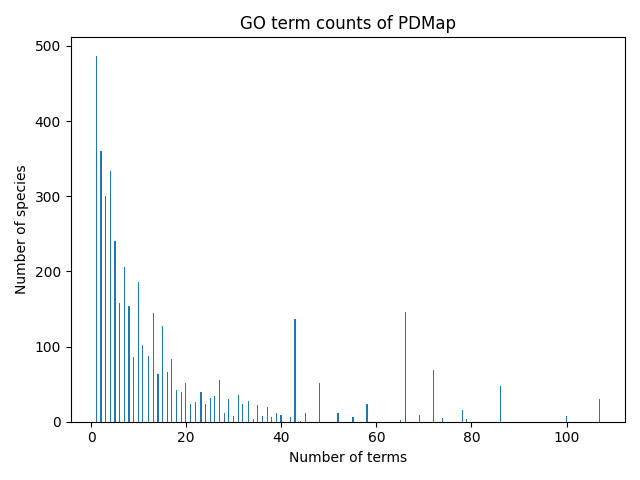
\includegraphics[width=0.48\linewidth]{go-term-counts-pdmap.png}
    \caption{Distribution of number of annotated GO terms per species in \PDMap{}.}
    \label{fig:go-term-counts}
  \end{figure}


We check the following combinations of features (see \reftab{feature-importance-features}):
\begin{itemize}
\item As a \cd{baseline} we use the same feature set as used in
  \refsec{TODO-importance of reorg steps}, i.e. \cd{basic-both}.
\item To assess the predictive value of the GO-based features in isolation, we consider
  \cd{constant-stddev} and \cd{constant-embed}: The features
  \cd{GO_stddev} and \cd{GO_embedding} as defined in
  \refsec{feature-selection} (the identifier ``constant'' comes from the fact
  that we additionally supply a meaningless single constant number as feature
  due to implementation purposes).
\item Additionally, we assess the GO-based features in combination with
  information on node degrees: \cd{degree-stddev} and \cd{degree-embed} consist
  of the \cd{degrees} feature set, plus \cd{GO_stddev} or \cd{GO_embedding}.
\end{itemize}
Since the embeddings are of relatively large dimensionality, to avoid making the
dimensionality of the final feature vector (in the sense of
\refsec{feature-selection}) exceedingly large, we avoid combining them with the
full set of all other available features.


\begin{figure}[h]
  \centering
  \begin{subfigure}{0.48\linewidth}
    \pic{annotations/results/comparison/roc-gnn-bak.png}
    \caption{TODO}
  \end{subfigure}
  \begin{subfigure}{0.48\linewidth}
    \pic{annotations/results/comparison/roc-svm-bak.png}
    \caption{TODO}
  \end{subfigure}
  \caption{(\ADLast $\rightarrow$ \PDMap{}; subsets) TODO}
  \label{fig:annotations-results}
\end{figure}

\paragraph{Results \& Discussion} Results are visualised in
\reffig{annotations-results}. Note that since we only consider the induced
subgraph or nodes for wich annotations are available, the training and
validation datasets are different from previous experiments.
% TODO mention that we use newer version PDMap but that this probably does not
% make a big difference
% TODO motivate why we only evaluate for PDMap19, why we have no annots for ReconMap

Neither approach seems to yield gains in classification performance. Indeed,
using GO-based features only yields performance not much better than that of a
random classifier. If combined with information on node degrees, model
performance stays the same in the best case and drops in other cases.

The implementation of this approach given here has several shortcomings:
\begin{itemize}
  \item It is species that are annotated with GO terms, but we map this
    information to species aliases. Thus, a species alias may be associated with
    GO terms that do not correspond do its graph neighbours in the diagram. This
    potentially leads to ambiguity. 
\item Many species are in fact annotated with more than just a few GO terms (see
  \reffig{go-term-counts}). It is unclear how specific or expressive many of
  these annotations are.
\item Aggregating several embedding vectors naively by taking their mean may be problematic.
\item Considering only species aliases for which annotations could be obtained
  further reduces the size of the dataset. This is potentially problematic for
  training the models. After subtracting excluded species, for \ADLast, there
  are $204$ aliases for prediction, $83$ of these are of positive class. For
  \PDMap{}, there are $802$ aliases for prediction, $209$ of these are of positive class.
  % determined via breakpoint in code...
\end{itemize}

One interesting observation is that, for the GNN model, the curves for
\cd{degree-embed} and \cd{degree-stddev} almost coincide, while for the SVM
model, there is a noticeable difference in the sense that additionally including
\cd{GO_embed} hurts model performance while providing \cd{GO_stddev}
does not.


% DONE svm with degrees actually yields .91 AUC, is that because of smaller
% dataset of because of combination of SVM and degrees? -- run
% feature-importance/degrees also with SVM
% --- no, not better, so prob just becaue of smaller datase t





\section{Additional Training Data}

...
% seems hard to find other maps that are somewhat comparable...
% TODO mention this in outlook?


\section{Attachment of Edges}
% TODO can we compare with the actual reattachment as done in the reorganisation
% steps? is this sth like 'enrichment analysis'? or could use comparison scores
% for clusterings like mutual information?

% TODO maybe plot number of duplicates for given disease maps

% TODO make clear that this could be used with other distances measures like on ostaszwewski_clustering

We apply the method to determine the number of duplicates and re-distribute
edges described in \refsec{edge-attachment} to the \textit{AlzPathway} map.

We provide some examples for successful and problematic cases in
\reffig{fig:neighb-clust-examples}. All nodes considered have positive
ground-truth class (i.e. are real duplication parents). From manual inspection,
the vast majority of results seemed to be reasonable clusterings, and in rare
cases, ambiguous situations like illustrated here occured.

% TODO maybe do comparison to *real* split? (or future work)

% TODO vertical alignment
\begin{figure}[h]
  \centering
  \begin{subfigure}{0.48\linewidth}
    % example where it works nicely
    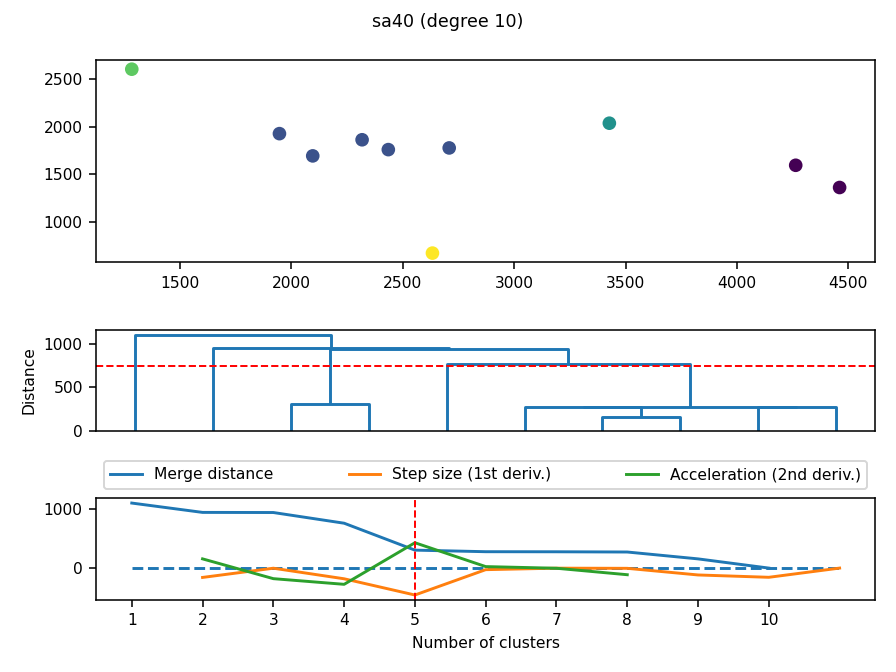
\includegraphics[width=1.0\textwidth]{dendrograms/sa40.png}
    \caption{
      Example for which the heuristic yields an intuitive clustering. Note that
      outliers do not distort the clustering result and are assigned their own cluster.
    }
    % sa40
  \end{subfigure}
  ~~~
  \begin{subfigure}{0.48\linewidth}
    % example where 2nd derivative is better than 1st (obs)
    % 220
    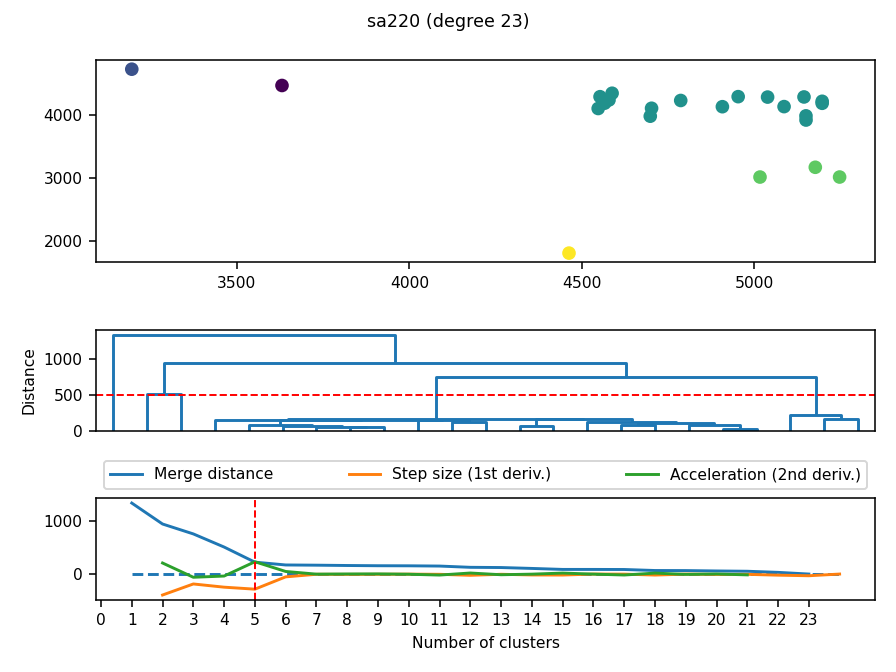
\includegraphics[width=\textwidth]{dendrograms/sa220.png}
    \caption{Example in which using the second derivative yields a clustering
      that intuitively seems more reasonable. The first derivative has its
      minimum
      % TODO should be maximum?
      at 2 clusters. 
    }
    % or 856
  \end{subfigure}
  \linebreak
      \begin{subfigure}{0.48\linewidth}
        % example where distributions are tricky (obs)
        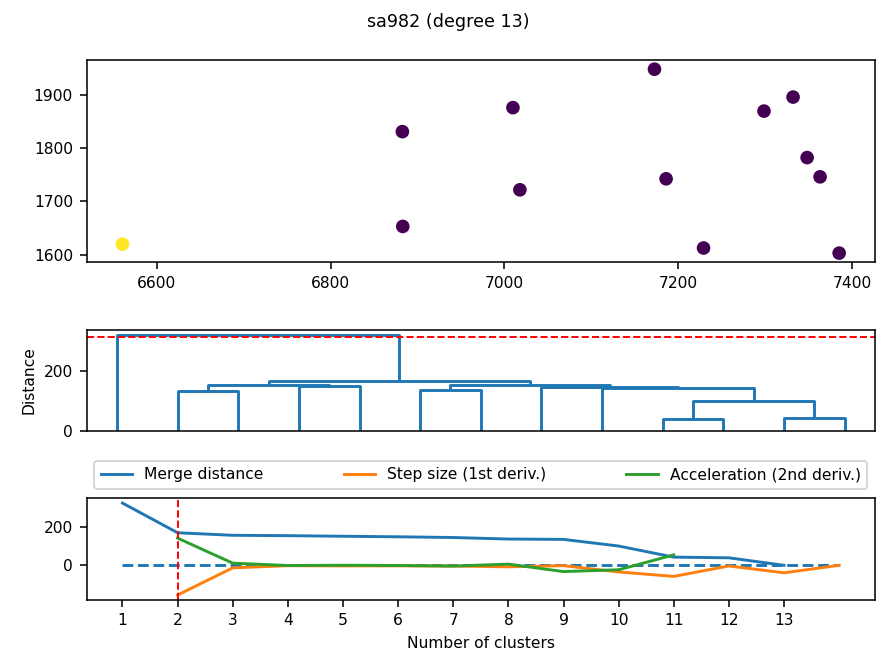
\includegraphics[width=\textwidth]{dendrograms/sa982.png}
        \caption{
          Distances between the purple points are not much
          different from the distance between the yellow point and the purple
          cluster (measured by \textit{single linkage}). While the heuristic yields
          only two clusters, it may have also been feasible to create many clusters.
          Indeed, the second derivative curve shows another local maximum at 11 clusters.
        }
        % or sa77
      \end{subfigure}
      ~~~
      \begin{subfigure}{0.48\linewidth}
        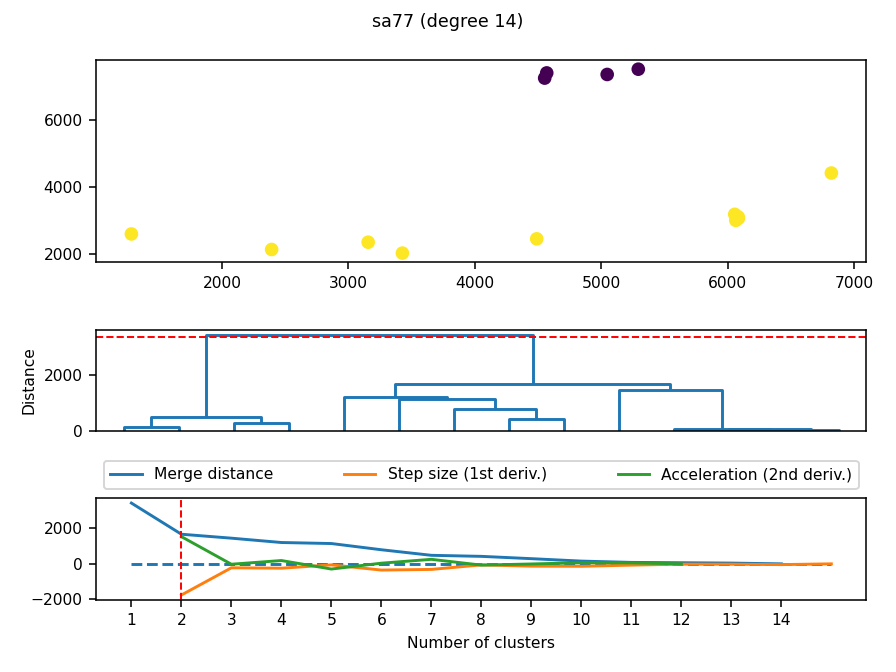
\includegraphics[width=\textwidth]{dendrograms/sa77-variance.png}
        \caption{Another example where large intra-cluster variance is
          problematic. Contrary to the heuristic's output, it may be preferrable
          to further split the yellow cluster.}
      \end{subfigure}
      \caption[
      Example outputs of the heuristic for attaching edges after node
      duplication has been decided.
      ]
      {
    Examples for the clustering procedure described in \refsec{edge-attachment}. The topmost scatterplot shows the positions of neighbours
    of a given node in the layout (given node and edges are not shown). Below, a clustering dendrogram describes
    the distances between two any clusters as they were merged. Finally, the
    sequence of merge distances as well as its first and second derivative.
    Taking the minumum, resp. maximum yields a hint for the number of clusters
    to choose. The red line indicates the suggested choice for the number of
    clusters and thus a concrete clustering, determing the merge node in the
    dendrogram where the ``cut'' should be made.
    % TODO reverse step size, should not be plotted as minimum here.
    All examples are from \ADLast{} with positive ground-truth label.}
  \label{fig:neighb-clust-examples}
\end{figure}


% ====================================
\chapter{Discussion}
\label{sec:discussion}

% TODO musings on definition of train/test tasks, internal split, more data

% ambuigity, difficulty
% (make sure we dont mention that too often...)
% - user study in nielsen et all even shows disagreement between experts

% TODO examine (mis)classifications


% ====================================
\chapter{Outlook \& Future Work}
\label{sec:future-work}

% more training data...


% positoning of duplicates

% using layout information
% - tension
% - stress
% need to take care that computed values are transferrable across maps


%  model learns while user is duplicating?

%  more data
%  - more disease maps
% - other kinds of networks (metabolic models)


% semi-supervised learning


% \citeauthor{tiezzi_GraphNeuralNetworks_2021} for node dup?

% GO annotations
% - semantic similarity
% - further ideas from mail from marek


% attachment of edges:
% semantic similarity for clustering


\pagebreak


\backmatter % Denotes the end of the main document content
\setchapterstyle{plain} % Output plain chapters from this point onwards

\appendix % From here onwards, chapters are numbered with letters, as is the appendix convention

\pagelayout{wide} % No margins


\chapter{Appendix}

\section{Notation \& Abbreviations}
\begin{itemize}
\item Vectors and matrices are usually set in bold letters, e.g. $\vec x$ or
  $\mat A$. Vectors are assumed to column vectors unless otherwise specified.
  $\cdot^T$ denotes the transpose.
\item $\norm{\cdot}$ denotes the $l_2$-norm, or set cardinality.
\item $G$ commonly denotes a graph, $V(G)$ is its vertex set and $E(G)$ its edge
  set. Whether we consider a directed, undirected, bipartite or simple graph
  will be made clear from context.
\item $\neighb(v)$ denotes the graph neighbourhood of node $v$. Unless otherwise
  specified, this is the direct 1-hop neighbourhood.
\item For a bipartite graph with node set $V = A
  \cupdot B$, that is, the disjoint union of species aliases $A$ and reactions
  $B$, the \ild{bipartite projection onto $A$} is the simple graph with node set
  $A$ in which $v_i, v_j \in A$ are connected if and only if in the bipartite
  they have a common neighbour in $B$.
\item A \ild{species} is an actor in a biological system. Examples for species
  are proteins, smaller molecules, but also drugs or phenotypes. A \ild{species
    alias} is a visual representation of a species in a drawing. If a disease map
  is interpreted as a graph, a species alias can be thought of as a node in the
  graph, see \refsec{graph-interpretation}. There can be multiple species
  aliases corresponding to the same species. A \ild{complex species alias}
  represents a collection of species aliases, commonly representing protein
  complexes.
\end{itemize}




\section{Acknowledgements}

Special thanks go to Sune S. Nielsen and Marek Ostaszewski for kindly answering
questions and being available for discussion. I also thank Karsten Klein,
Matthias Rupp and particularly Michael Aichem for providing me with valuable
feedback, guiding me through the process and simply being great people to work
with.



% \pagelayout{margin} % Restore margins

%----------------------------------------------------------------------------------------


%----------------------------------------------------------------------------------------
%	BIBLIOGRAPHY
%----------------------------------------------------------------------------------------

% The bibliography needs to be compiled with biber using your LaTeX editor, or on the command line with 'biber main' from the template directory

% \defbibnote{bibnote}{Here are the references in citation order.\par\bigskip} % Prepend this text to the bibliography
% \printbibliography[heading=bibintoc, title=References, prenote=bibnote] % Add the bibliography heading to the ToC, set the title of the bibliography and output the bibliography note
\renewcommand*{\bibfont}{\small}
\printbibliography[heading=bibintoc, title=References] % Add the bibliography heading to the ToC, set the title of the bibliography and output the bibliography note

%----------------------------------------------------------------------------------------
%	INDEX
%----------------------------------------------------------------------------------------

% The index needs to be compiled on the command line with 'makeindex main' from the template directory

\printindex % Output the index

\end{document}
